%% ACM Large 1-Column Format - Official Template
\documentclass[acmlarge,screen,nonacm]{acmart}

%% Remove ACM copyright and other info for student projects
\setcopyright{none}
\settopmatter{printacmref=false}
\renewcommand\footnotetextcopyrightpermission[1]{}
\pagestyle{plain}

%% Additional packages
\usepackage{listings}
\usepackage{subcaption}
\usepackage{float}  
\usepackage{placeins}
\usepackage{hyperref}


%% Code listing settings
\lstset{
  language=Python,
  basicstyle=\ttfamily\small,
  keywordstyle=\color{blue},
  commentstyle=\color{green!60!black},
  stringstyle=\color{orange},
  breaklines=true,
  frame=single,
  numbers=left,
  numberstyle=\tiny\color{gray}
}

%%
%% Title and Author Information
%%
\title{ML4N - SSH Shell Attack Analysis}

\author{Sattar Aftabi Amaneh}
\affiliation{%
  \institution{Politecnico di Torino}
  \city{Turin}
  \country{Italy}
}

\author{Donya Mohebi}
\affiliation{%
  \institution{Politecnico di Torino}
  \city{Turin}
  \country{Italy}
}

\author{Michele Valerio}
\affiliation{%
  \institution{Politecnico di Torino}
  \city{Turin}
  \country{Italy}
}

\author{Thiago Ricardo}
\affiliation{%
  \institution{Politecnico di Torino}
  \city{Turin}
  \country{Italy}
}

%%
%% Abstract
%%
\begin{abstract}    
This paper presents a comprehensive machine learning approach to analyze SSH shell attack sessions collected from honeypot systems. Using a dataset of 233,035 unique Unix shell attack sessions spanning from June 2019 to February 2020, we developed a multi-faceted methodology combining supervised learning, unsupervised clustering, and advanced language models to classify attacker tactics based on the MITRE ATT\&CK framework. 

The key contributions of this work include: (1) development of a robust preprocessing pipeline analyzing temporal trends, extracting numerical features, and evaluating intent distributions from large-scale SSH attack session data; (2) implementation of supervised classification models (Logistic Regression and SVM) with hyperparameter tuning achieving micro F1-scores above 0.99 and macro F1-scores of 0.846 for multi-label intent prediction; (3) application of unsupervised clustering techniques (K-Means with k=10 and Agglomerative Hierarchical Clustering) to uncover hidden patterns in attack behaviors with cluster purity scores of 97.75\%; and (4) comparative evaluation of BERT-based language models against traditional ML approaches for intent classification. 

Our analysis reveals that Discovery and Persistence are the dominant attack intents, often occurring together, while extreme class imbalance remains the primary challenge limiting performance on rare intents. Traditional machine learning with carefully tuned Logistic Regression achieves superior overall performance compared to BERT, demonstrating that proper feature engineering and class weighting are more effective than architectural sophistication when discriminative lexical features exist.
\end{abstract}

%%
%% Keywords
%%
\keywords{Machine learning, supervised learning, unsupervised learning, language models, text classification, clustering, intent classification, SSH shell attacks, security log analysis, MITRE ATT\&CK}

%%
%% Start of document
%%
\begin{document}

%%
%% CCS Concepts (ACM Classification) - Must be after \begin{document}
%%
\begin{CCSXML}
<ccs2012>
   <concept>
       <concept_id>10002978.10002997.10002998</concept_id>
       <concept_desc>Security and privacy~Intrusion detection systems</concept_desc>
       <concept_significance>500</concept_significance>
       </concept>
   <concept>
       <concept_id>10010147.10010257</concept_id>
       <concept_desc>Computing methodologies~Machine learning</concept_desc>
       <concept_significance>500</concept_significance>
       </concept>
   <concept>
       <concept_id>10010147.10010257.10010293.10010294</concept_id>
       <concept_desc>Computing methodologies~Neural networks</concept_desc>
       <concept_significance>300</concept_significance>
       </concept>
    <concept>
       <concept_id>10010147.10010257.10010258.10010259</concept_id>
       <concept_desc>Computing methodologies~Unsupervised learning</concept_desc>
       <concept_significance>300</concept_significance>
       </concept>
 </ccs2012>
\end{CCSXML}

\ccsdesc[500]{Security and privacy~Intrusion detection systems}
\ccsdesc[500]{Computing methodologies~Machine learning}
\ccsdesc[300]{Computing methodologies~Neural networks}
\ccsdesc[300]{Computing methodologies~Unsupervised learning}

\maketitle

% ============================================
% SECTION 1: INTRODUCTION AND BACKGROUND
% ============================================
\section{Introduction}

\subsection{Motivation}

Security logs play a crucial role in understanding and mitigating cyber attacks, particularly in the domain of network and system security. With the increasing sophistication of cyber threats, analyzing and interpreting security logs has become paramount for detecting, preventing, and responding to potential security breaches. Unix shell attacks, especially those executed through the SSH protocol, represent a significant vector for potential system compromises.

The complexity of security log analysis stems from several key challenges:
\begin{itemize}
    \item Logs are often unstructured and contain ambiguous or malformed text
    \item Manual parsing and interpretation of logs is time-consuming and error-prone
    \item The sheer volume of log data makes comprehensive manual review impractical
    \item Multi-label nature of attacks where single sessions exhibit multiple tactics simultaneously
\end{itemize}

These challenges underscore the need for automated, intelligent approaches to log analysis that can efficiently extract meaningful insights and identify potential security threats.

\subsection{Objective}

The primary objective of this research is to develop and evaluate machine learning techniques for automatic analysis and classification of SSH shell attack logs. Specifically, we aim to:

\begin{itemize}
    \item Automate multi-label intent classification using MITRE ATT\&CK framework
    \item Compare traditional machine learning approaches with modern language models to identify optimal solutions for production deployment
    \item Discover latent attack patterns through unsupervised clustering to reveal attacker strategies beyond labeled intents
    \item Provide security professionals with actionable insights into attack behaviors, temporal patterns, and threat prioritization
    \item Evaluate the impact of extreme class imbalance on model performance and identify effective mitigation strategies
\end{itemize}

The significance of this research lies in its potential to enhance cybersecurity threat detection and response capabilities by transforming complex, unstructured log data into actionable intelligence. By systematically comparing supervised classification, unsupervised pattern discovery, and advanced language models, this work provides practical guidance for deploying ML-powered log analysis systems in real-world security operations.

\subsection{MITRE ATT\&CK Framework}

The MITRE ATT\&CK (Adversarial Tactics, Techniques, and Common Knowledge) framework provides a comprehensive knowledge base of adversary tactics and techniques observed in real-world cyber attacks. This framework serves as a standardized methodology for understanding and categorizing attack strategies.

For our research, we focus on seven key intents derived from the MITRE ATT\&CK framework:
\begin{itemize}
    \item \textbf{Persistence}: Methods adversaries use to maintain access to systems after restarts or credential changes
    \item \textbf{Discovery}: Techniques for gathering information about the target system and network environment
    \item \textbf{Defense Evasion}: Strategies to avoid detection by security mechanisms
    \item \textbf{Execution}: Techniques for running malicious code on target systems
    \item \textbf{Impact}: Actions aimed at manipulating, interrupting, or destroying systems and data
    \item \textbf{Other}: Less common tactics including Reconnaissance, Resource Development, Initial Access, etc.
    \item \textbf{Harmless}: Non-malicious code or actions
\end{itemize}

\subsection{Research Approach}

Our research employs a multi-faceted approach combining four complementary methodologies:

\begin{enumerate}
    \item \textbf{Data Exploration and Preprocessing}: 
    \begin{itemize}
        \item Analysis of 233,035 SSH attack sessions with temporal trend identification
        \item Feature extraction using TF-IDF vectorization for command-based representations
        \item Investigation of extreme class imbalance across seven MITRE ATT\&CK intent categories
    \end{itemize}
    
    \item \textbf{Supervised Learning for Intent Classification}:
    \begin{itemize}
        \item Implementation and comparison of traditional ML models (e.g., tuned Logistic Regression)
        \item Comprehensive hyperparameter tuning with cross-validation
        \item Evaluation of class weighting strategies to address minority class challenges
    \end{itemize}
    
    \item \textbf{Unsupervised Clustering for Pattern Discovery}:
    \begin{itemize}
        \item Application of K-Means and Agglomerative Hierarchical Clustering
        \item Optimal cluster selection using multiple evaluation metrics
        \item Analysis of cluster-intent relationships to validate discovered patterns
    \end{itemize}
    
    \item \textbf{Language Model Exploration}:
    \begin{itemize}
        \item Fine-tuning BERT for multi-label SSH attack classification
        \item Comparative evaluation against traditional ML to assess transfer learning benefits, despite computational trade-offs
        \item Analysis of efficiency metrics (training time, inference latency, model size)
    \end{itemize}
\end{enumerate}

This comprehensive methodology enables us to identify the most effective approaches for SSH attack analysis while providing insights into the strengths and limitations of each technique in the context of security log analysis.

\subsection{Related Work}

Security log analysis has evolved significantly with advances in machine learning. Honeypot systems like those described by Provos~\cite{honeypot_ssh} have become essential for collecting real-world attack data, enabling data-driven security research. Traditional signature-based intrusion detection systems struggle with novel attacks, motivating the shift toward behavioral analysis using machine learning~\cite{intrusion_detection_ml}.

Recent work in log analysis has demonstrated the effectiveness of deep learning approaches. Du et al.~\cite{log_analysis_ml} applied LSTMs to system logs for anomaly detection, while transformer-based models like BERT have shown promise in understanding command sequences and security contexts. Multi-label classification in security domains presents unique challenges due to class imbalance and overlapping attack tactics~\cite{tsoumakas2007multi}.

Our work extends this body of research by combining traditional ML, unsupervised clustering, and BERT-based language models specifically for SSH attack analysis mapped to the MITRE ATT\&CK framework. This multi-faceted approach enables both automated classification and discovery of novel attack patterns, addressing gaps in purely supervised or unsupervised methodologies. Building on this foundation, the following sections detail our methodology, experimental results, and key findings.

% ============================================
% SECTION 2: DATA EXPLORATION AND PREPROCESSING
% ============================================
\section{Data Exploration and Preprocessing}

\subsection{Dataset Overview}

The dataset consists of SSH attack logs from honeypot systems, with each entry including:
\begin{itemize}
    \item \texttt{session\_id}: Unique integer identifier
    \item \texttt{full\_session}: Command sequence (string)
    \item \texttt{first\_timestamp}: Session start (datetime)
    \item \texttt{Set\_Fingerprint}: MITRE ATT\&CK labels (multi-label)
\end{itemize}

It contains \textbf{233,035 unique sessions} from June 2019 to February 2020, offering a rich view of SSH attack patterns.

\subsection{Dataset Preparation and Feature Extraction}

The Parquet file was preprocessed as follows:
\begin{enumerate}
    \item Decode \texttt{full\_session} to readable format
    \item Convert \texttt{first\_timestamp} to datetime
    \item Split sessions using ;, |, and whitespace
    \item Clean commands with regex to remove symbols/assignments
    \item Check for missing values (none found)
\end{enumerate}

Example raw: \begin{lstlisting}[language=bash]
enable ; system ; shell ; sh ; cat /proc/mounts ; 
/bin/busybox SAEMW ; cd /dev/shm ; cat .s || cp /bin/echo .s
\end{lstlisting}

Processed: \begin{lstlisting}[language=Python]
[enable, system, shell, sh, cat, /proc/mounts, /bin/busybox, 
SAEMW, cd, /dev/shm, cat, .s, cp, /bin/echo, .s, ...]
\end{lstlisting}

\subsection{Temporal Analysis}

Attacks show continuous activity with notable patterns:
\begin{itemize}
    \item Surge mid-October 2019 to January 2020, peaking December (\textasciitilde78,000)
    \item Uniform across days, slightly higher weekdays (Monday max \textasciitilde35,000)
    \item Evening concentration (\textasciitilde21:00 UTC peak \textasciitilde10,000), suggesting automated bots
\end{itemize}

Figure~\ref{fig:temporal_grid} captures these trends, highlighting 24/7 operations.

\begin{figure}[h]
\centering
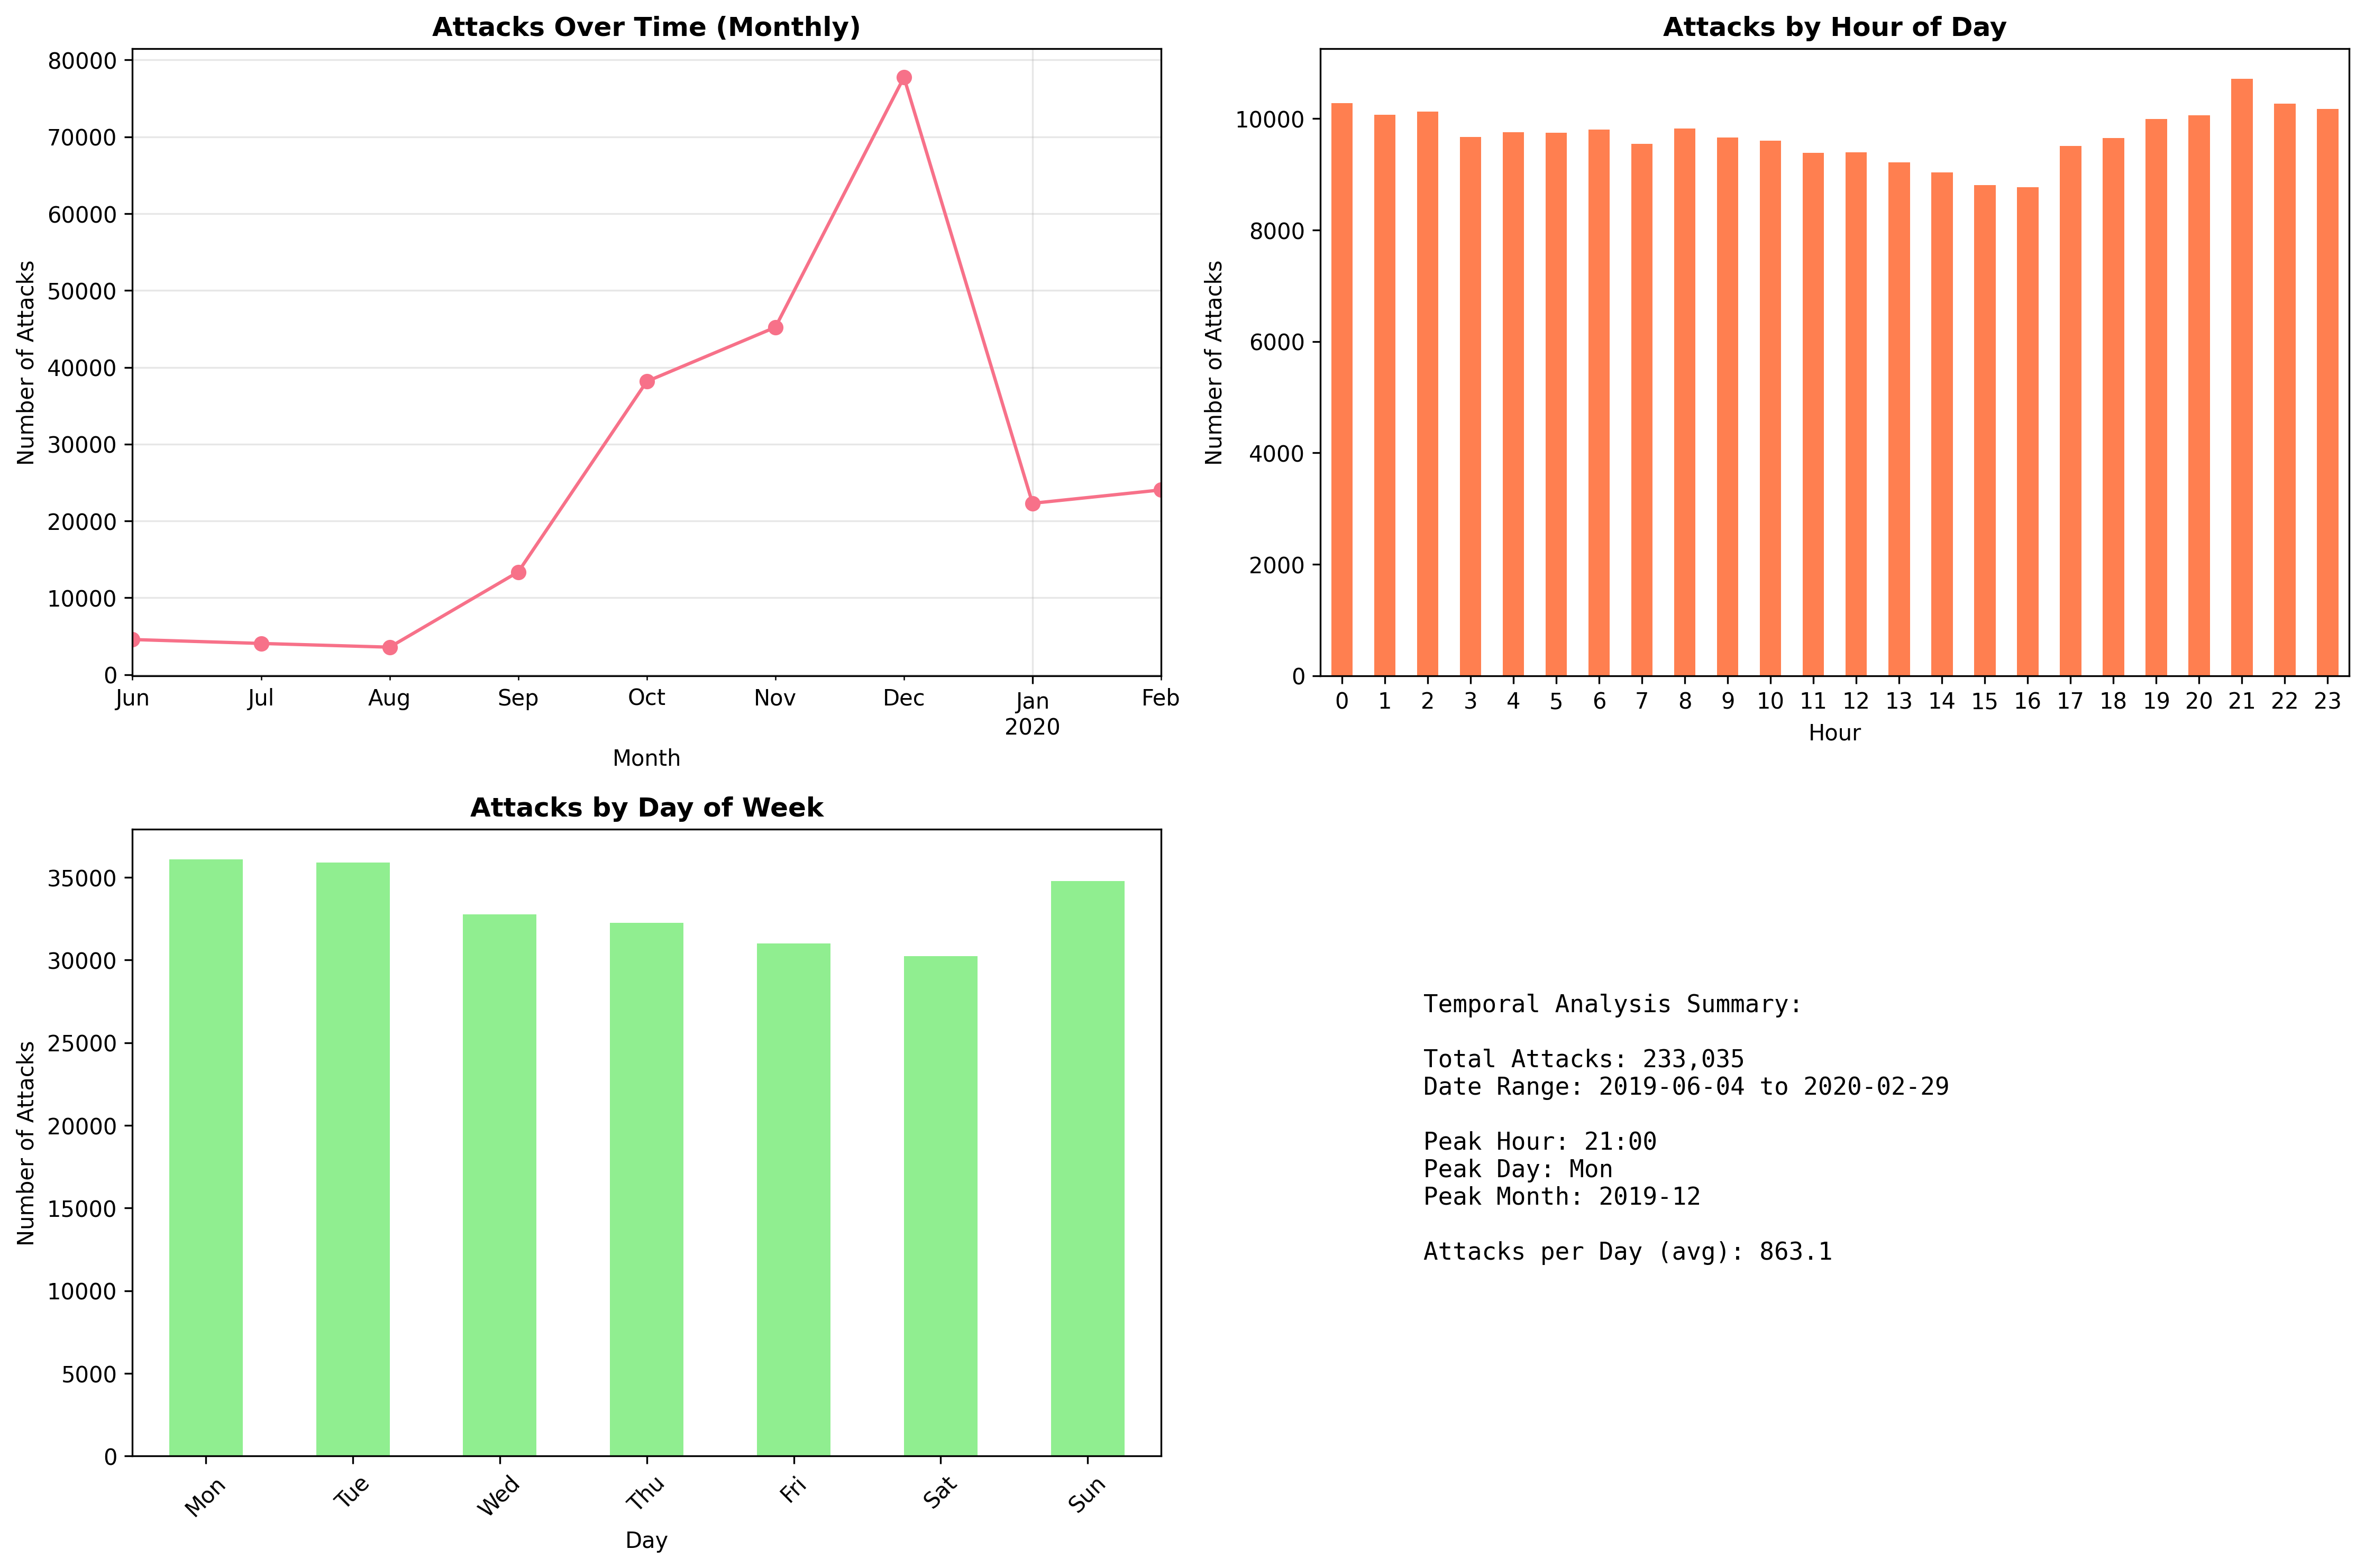
\includegraphics[width=0.75\textwidth]{results/plots/section1/temporal_analysis_grid.png}
\caption{Temporal attack distribution: Monthly peaks December 2019; hourly evening bias; weekday slight increase.}
\label{fig:temporal_grid}
\end{figure}

\subsection{Session Characteristics Analysis}

Sessions vary widely: median 116 words (mean 121) and 620 characters (mean 1,014), with complex attacks reaching 35,000+ words and 200,000+ characters due to long-tail distribution. This diversity reflects simple probes to multi-stage scripts. See \hyperref[appendix:A1]{Appendix A.1} for distributions.

\subsection{Vocabulary Analysis}

Recon commands dominate (grep, cat, echo, uname), with paths like /proc/cpuinfo for fingerprinting. TF-IDF representation effectively captured discriminative patterns, reducing dimensionality from ~300,000 unique tokens to 5,000 most informative features (min\_df=5, max\_features=5000). See \hyperref[appendix:A2]{Appendix A.2} for top tokens.

\subsection{Intent Distribution Analysis}

Figure~\ref{fig:num_intents} shows most sessions have 2-3 intents (98.3\%), averaging 2.39. Figure~\ref{fig:intent_dist} highlights imbalance: Discovery (232,145, 99.6\%), Persistence (211,295, 90.7\%), Execution (92,927, 39.9\%), Defense Evasion (18,999, 8.2\%), Harmless (2,206, 0.95\%), Other (327, 0.14\%), Impact (27, 0.01\%). Discovery/Persistence often co-occur.

Temporal evolution (\hyperref[appendix:A3]{Appendix A.3}) shows stable majors, with Execution/Impact spiking December 2019.

\begin{figure}[htbp]
\centering
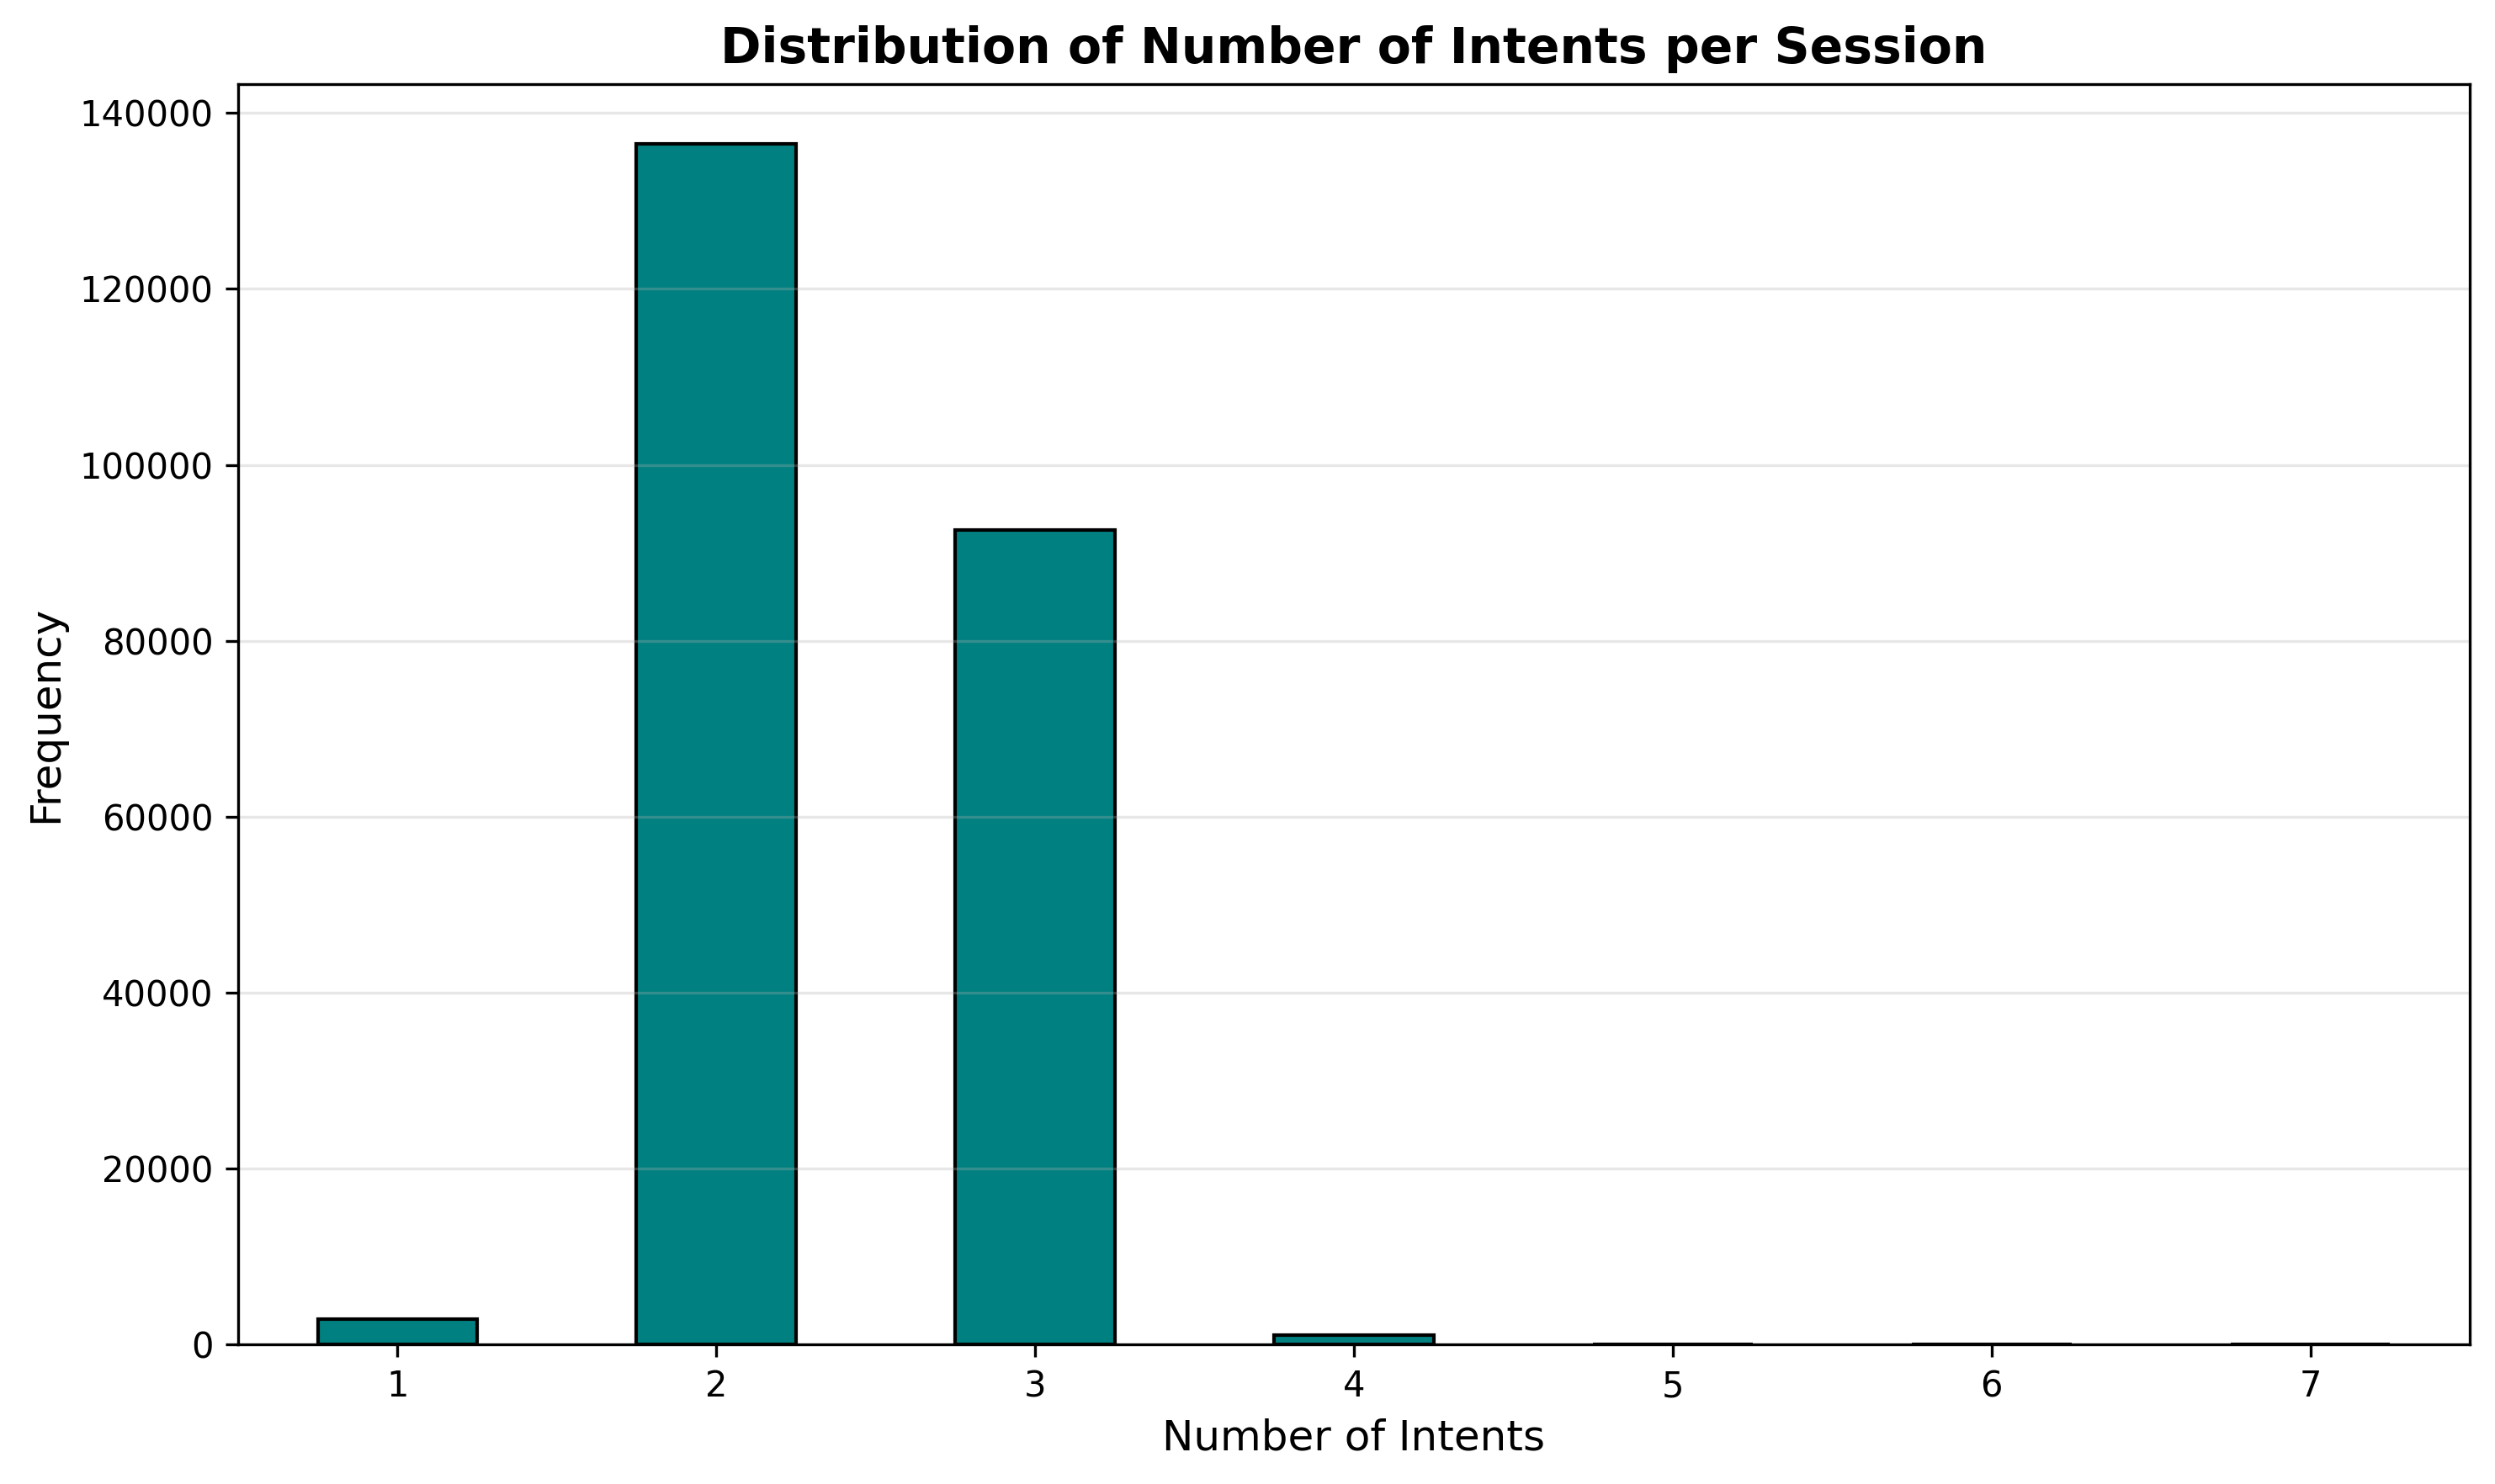
\includegraphics[width=0.65\textwidth]{results/plots/section1/num_intents_distribution.png}
\caption{Multi-label distribution: 58.6\% 2 intents, 39.7\% 3, rare singles (1.3\%) or 4+ (0.5\%).}
\label{fig:num_intents}
\end{figure}

\begin{figure}[htbp]
\centering
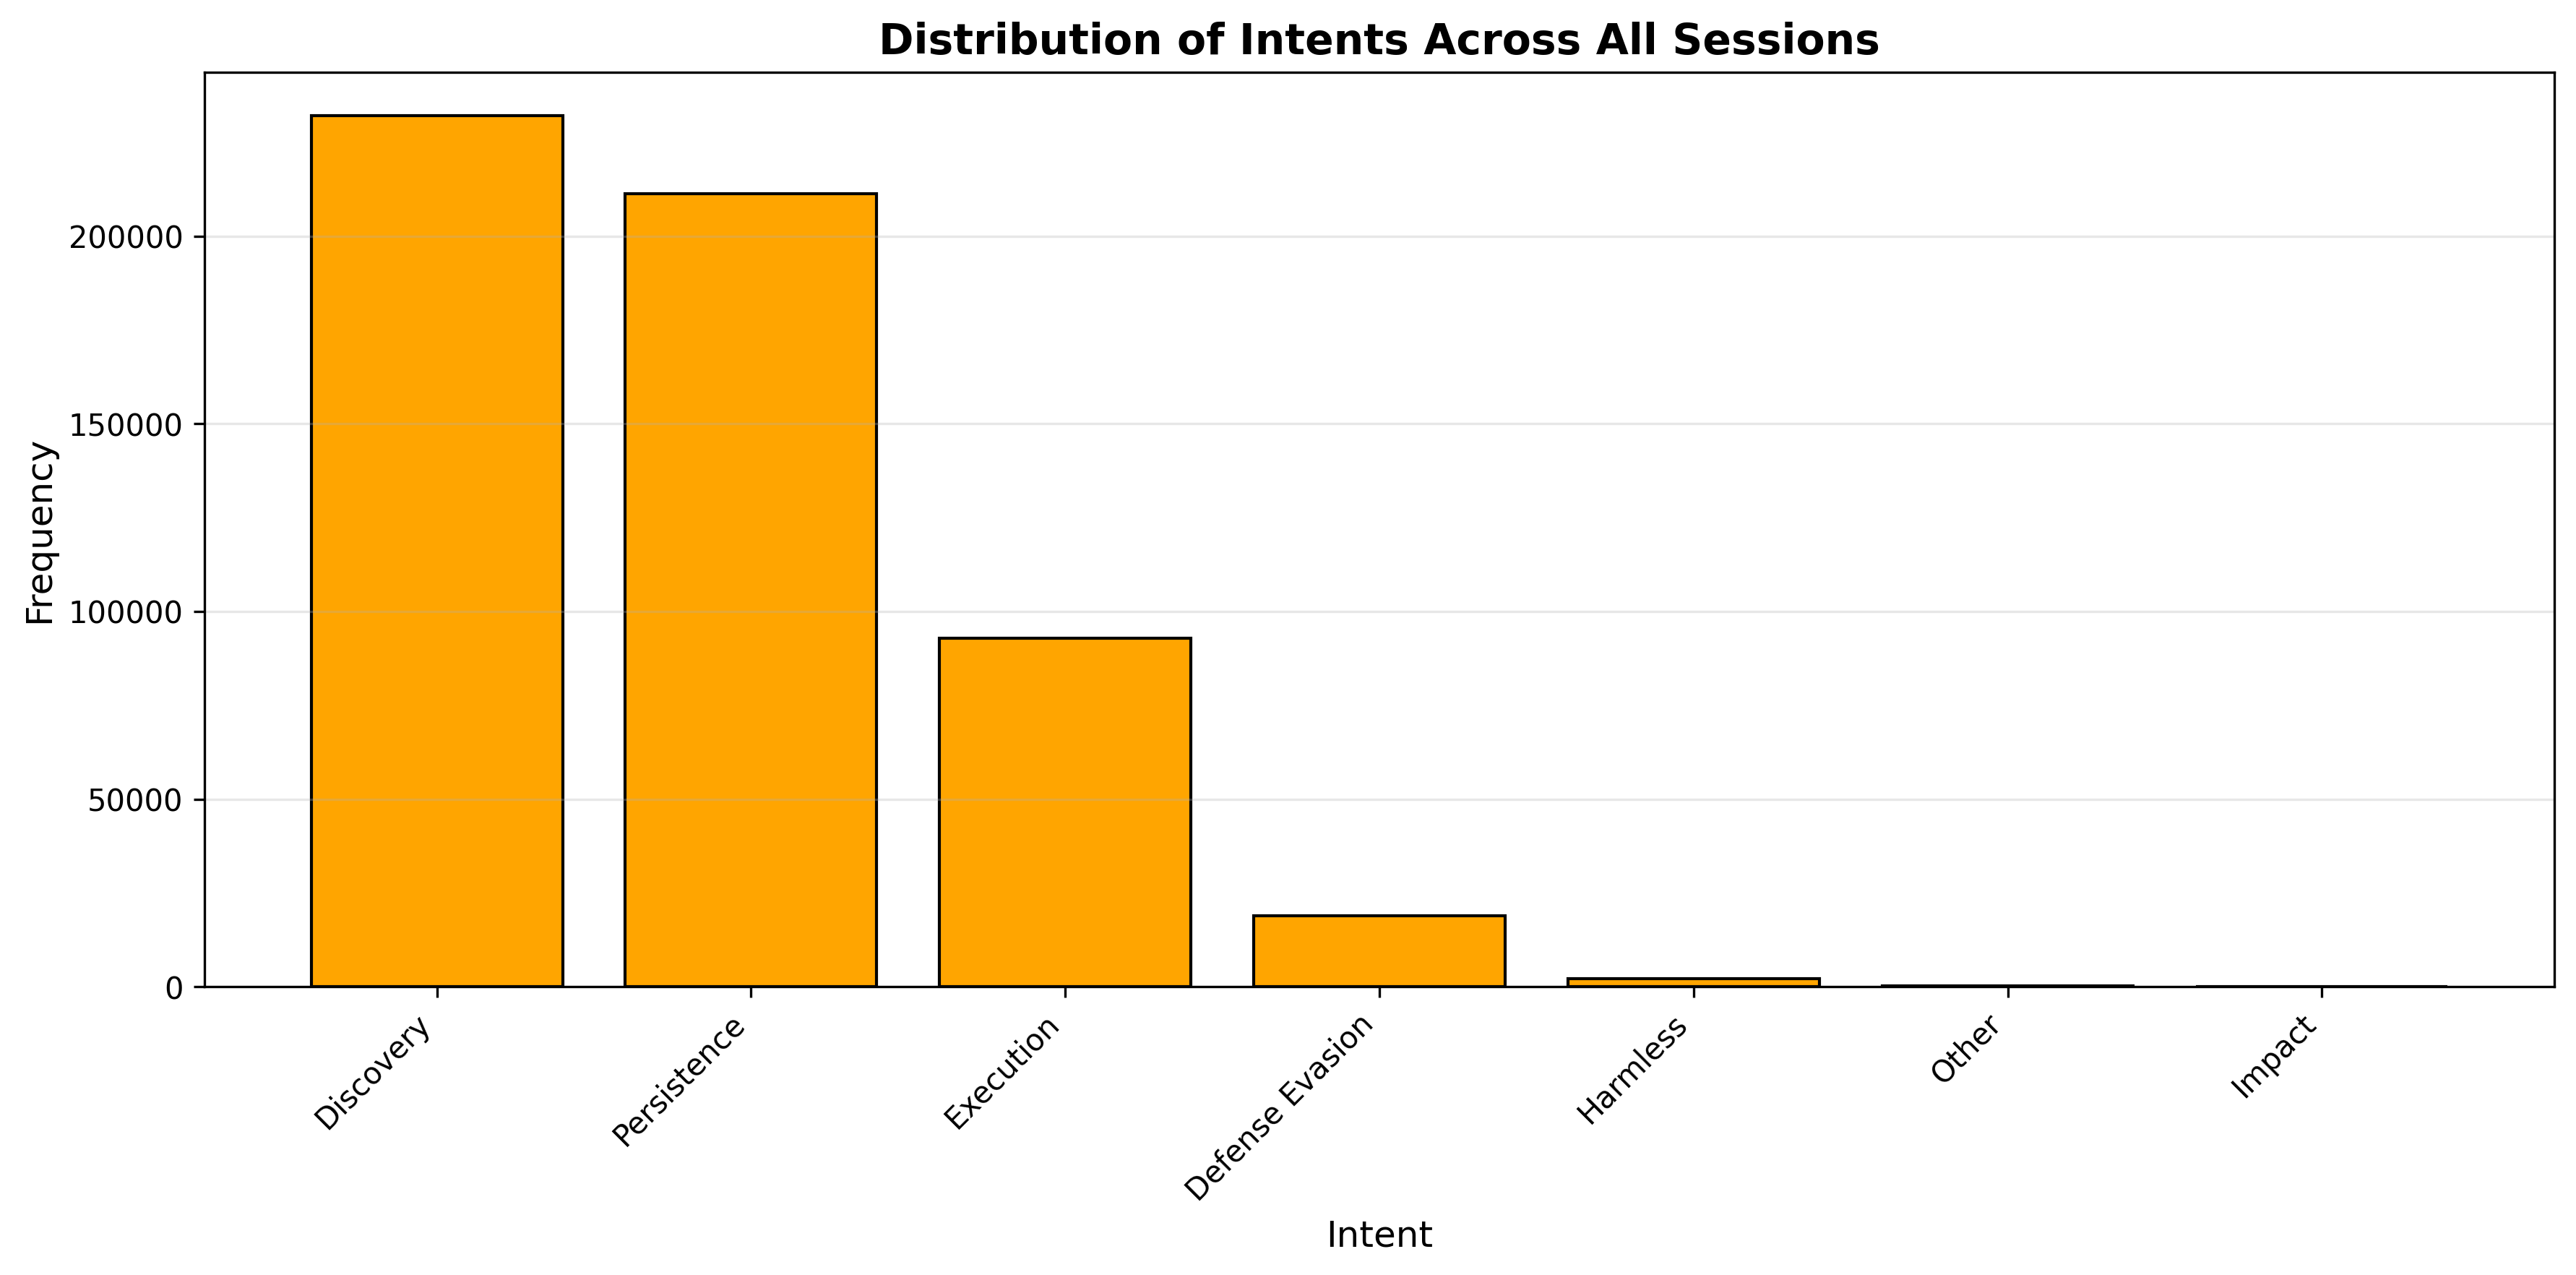
\includegraphics[width=0.7\textwidth]{results/plots/section1/intent_distribution.png}
\caption{Intent occurrence frequencies showing severe class imbalance. Discovery (99.6\%) and Persistence (90.7\%) dominate, while Impact (0.01\%) is extremely rare.}
\label{fig:intent_dist}
\end{figure}

\FloatBarrier

\subsection{Text Representation}

Bag of Words (BoW) represents sessions as frequency vectors but ignores term importance. TF-IDF extends BoW by weighting terms based on inverse document frequency:

\begin{equation}
\text{TF-IDF}(t, d, D) = \text{TF}(t, d) \times \log\left(\frac{|D|}{|\{d : t \in d\}|}\right)
\end{equation}

TF-IDF representation effectively captured discriminative attack patterns, reducing dimensionality from approximately 300,000 unique tokens to 5,000 most informative features through filtering (min\_df=5) and selection (max\_features=5000). This TF-IDF representation with 5,000 features was used for all subsequent supervised classification and unsupervised clustering tasks, providing an optimal balance between feature expressiveness and computational tractability.

% ============================================
% SECTION 3: SUPERVISED LEARNING - CLASSIFICATION
% ============================================
\section{Supervised Learning - Classification}

\subsection{Problem Formulation}

This task is multi-label classification of sessions into MITRE ATT\&CK intents, where each can have multiple labels:
\begin{itemize}
    \item \textbf{Strategy}: Binary Relevance for independent predictions
    \item \textbf{Features}: TF-IDF vectors (5,000 dimensions)
    \item \textbf{Split}: 80\% train (186,428 sessions), 20\% test (46,607)
    \item \textbf{Metrics}: Precision, Recall, F1 (Micro/Macro), Hamming Loss
\end{itemize}

\subsection{Models and Methodology}

We evaluated two models for multi-label classification using One-vs-Rest strategy:

\paragraph{Logistic Regression} as baseline linear classifier:
\begin{itemize}
    \item One-vs-Rest for multi-label
    \item L2 regularization (C=1.0 default)
    \item max\_iter=1000 for convergence
    \item lbfgs solver for efficiency
    \item random\_state=42 for reproducibility
\end{itemize}

\paragraph{Linear SVM} for efficient linear classification on high-dimensional text features::
\begin{itemize}
    \item One-vs-Rest for multi-label
    \item Linear kernel (suitable for high-dimensional TF-IDF features)
    \item Regularization parameter C=1.0
    \item Balanced class weights to handle imbalance
    \item random\_state=42 for reproducibility
\end{itemize}

\paragraph{Hyperparameter Tuning} via GridSearchCV (5-fold CV, scoring='f1\_macro'):
\begin{itemize}
    \item LR: C $\in \{0.1, 1, 10\}$, penalty $\in \{\text{'l1'}, \text{'l2'}\}$ (with solver='liblinear' for l1)
    \item SVM: C $\in \{0.1, 1, 10\}$
\end{itemize}

\subsection{Feature Importance Analysis}

As shown in \hyperref[appendix:B1]{Appendix B.1}, top features include obfuscated terms (/var/tmp paths) for persistence, 'admin'/'passwd' for evasion, and 'bash'/'echo' for execution—unveiling how attackers hide in plain sight through common yet telling commands.

\subsection{Model Performance Evaluation}

Table~\ref{tab:classification_results} compares models. Figure~\ref{fig:confusion_matrices} shows LR confusion matrices; Figure~\ref{fig:per_intent_f1} details per-intent F1.

\begin{table}[h]
\centering
\caption{Classification Model Performance Comparison}
\label{tab:classification_results}
\begin{tabular}{@{}lcccc@{}}
\toprule
\textbf{Model} & \textbf{Accuracy} & \textbf{F1 (Micro)} & \textbf{F1 (Macro)} & \textbf{Hamming Loss} \\
\midrule
Logistic Regression (baseline) & 0.9818 & 0.9958 & 0.7274 & 0.0182 \\
Random Forest (baseline) & 0.9844 & 0.9964 & 0.8451 & 0.0156 \\
Logistic Regression (tuned) & 0.9843 & 0.9964 & 0.8463 & 0.0157 \\
Random Forest (tuned) & 0.9835 & 0.9963 & 0.7511 & 0.0165 \\
Logistic Regression (BoW) & 0.9845 & 0.9965 & 0.7527 & 0.0155 \\
\bottomrule
\end{tabular}
\end{table}

\begin{figure}[htbp]
\centering
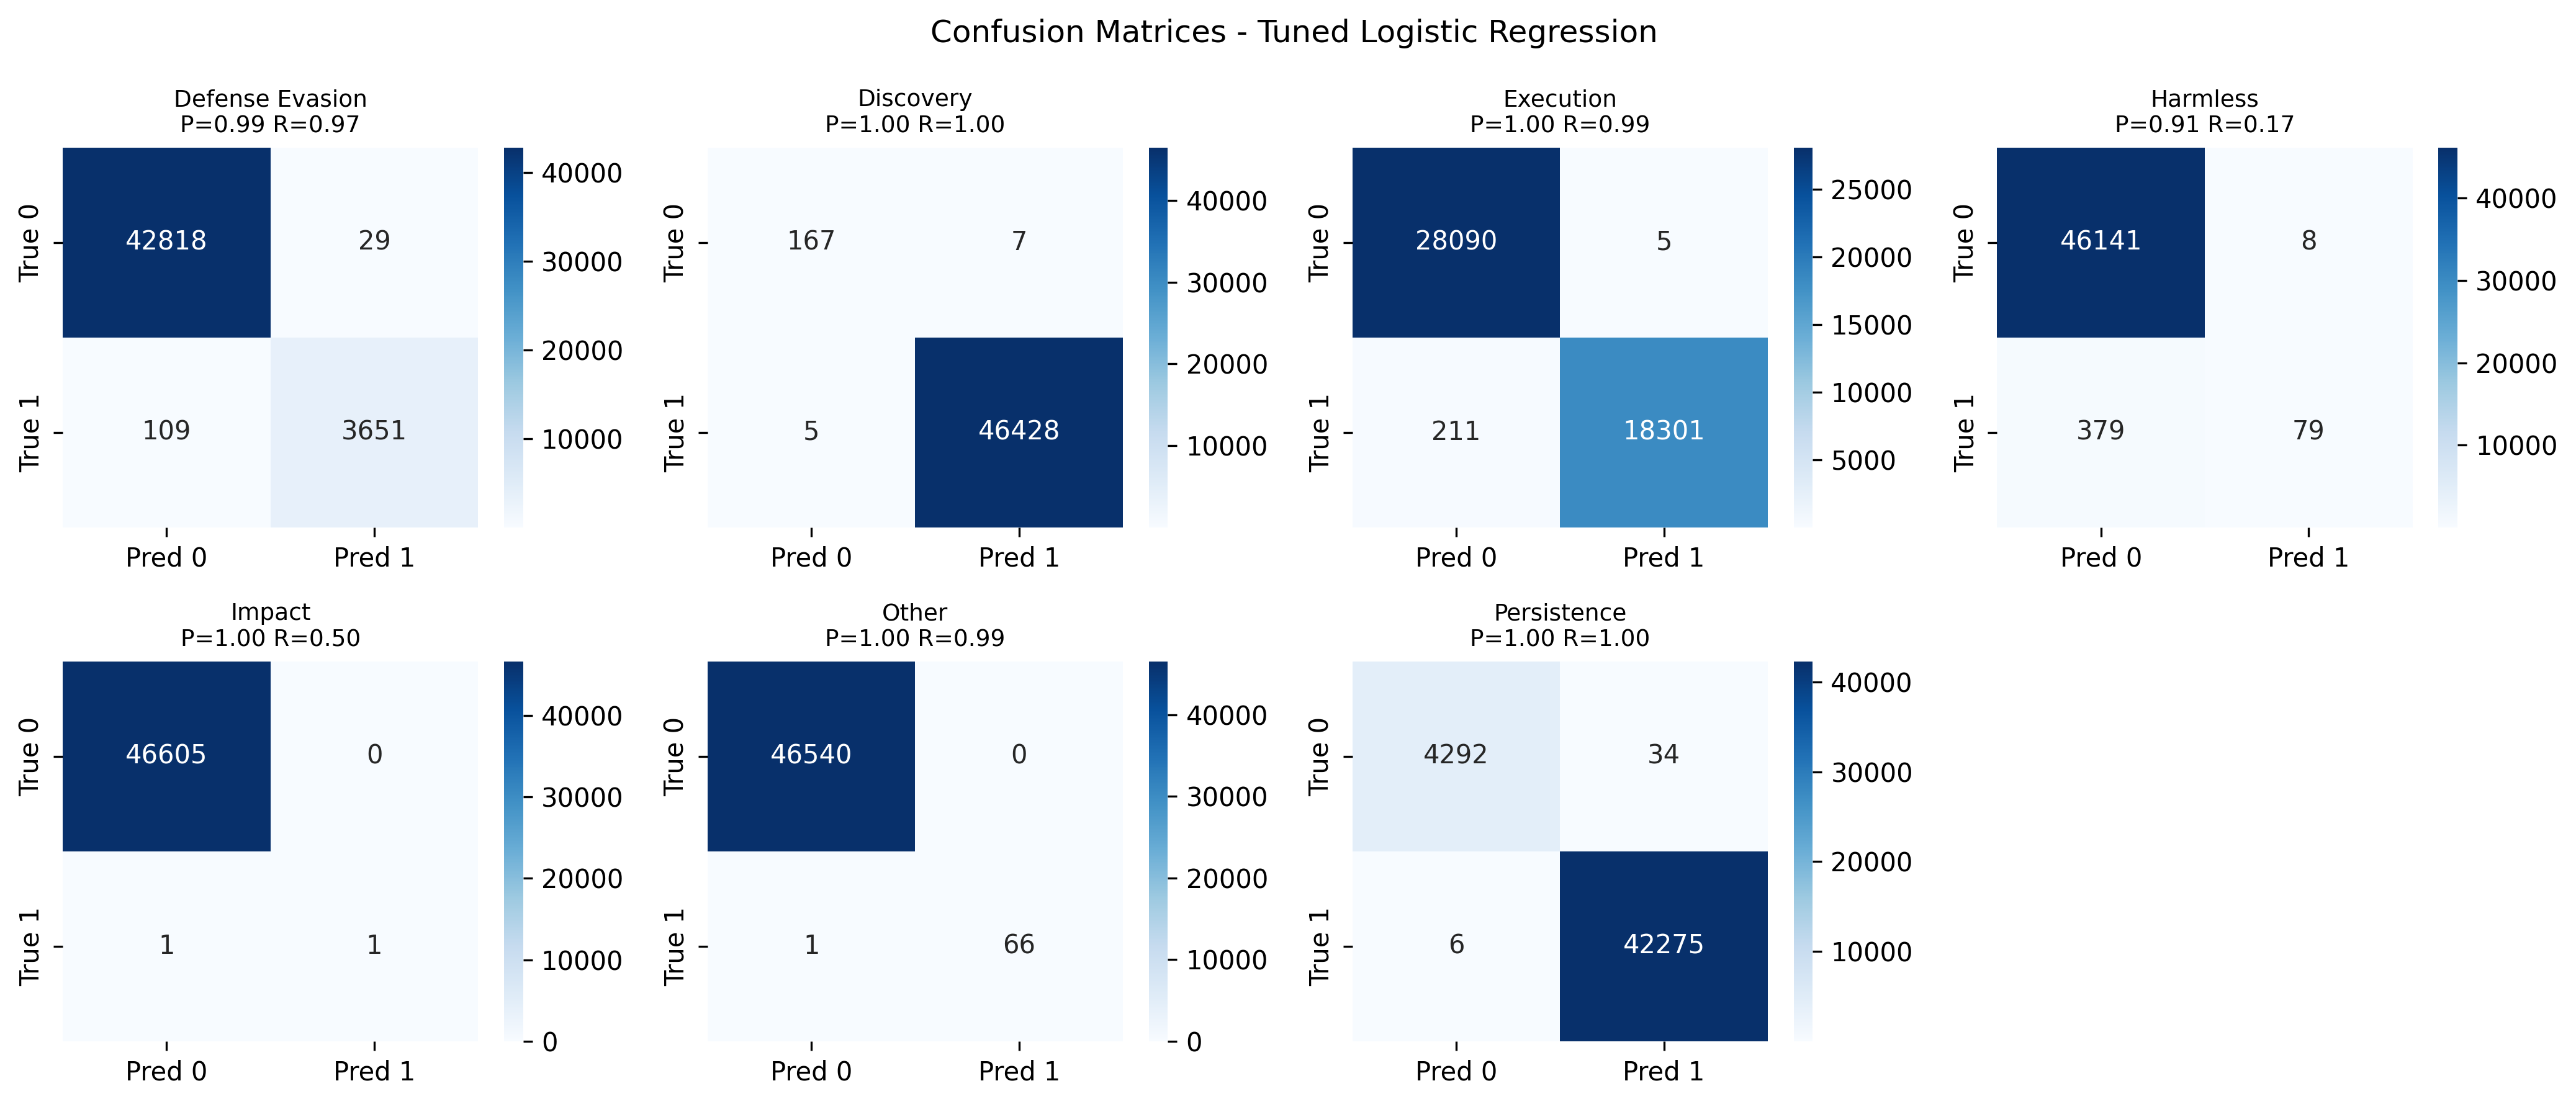
\includegraphics[width=0.75\textwidth]{results/plots/section2/confusion_matrices.png}
\caption{Confusion matrices for tuned Logistic Regression across intents. Strong diagonals for majors (Discovery/Persistence >90\% TP); minorities like Impact show FNs, often misclassified as Execution due to command overlap.}
\label{fig:confusion_matrices}
\end{figure}

\begin{figure}[htbp]
\centering
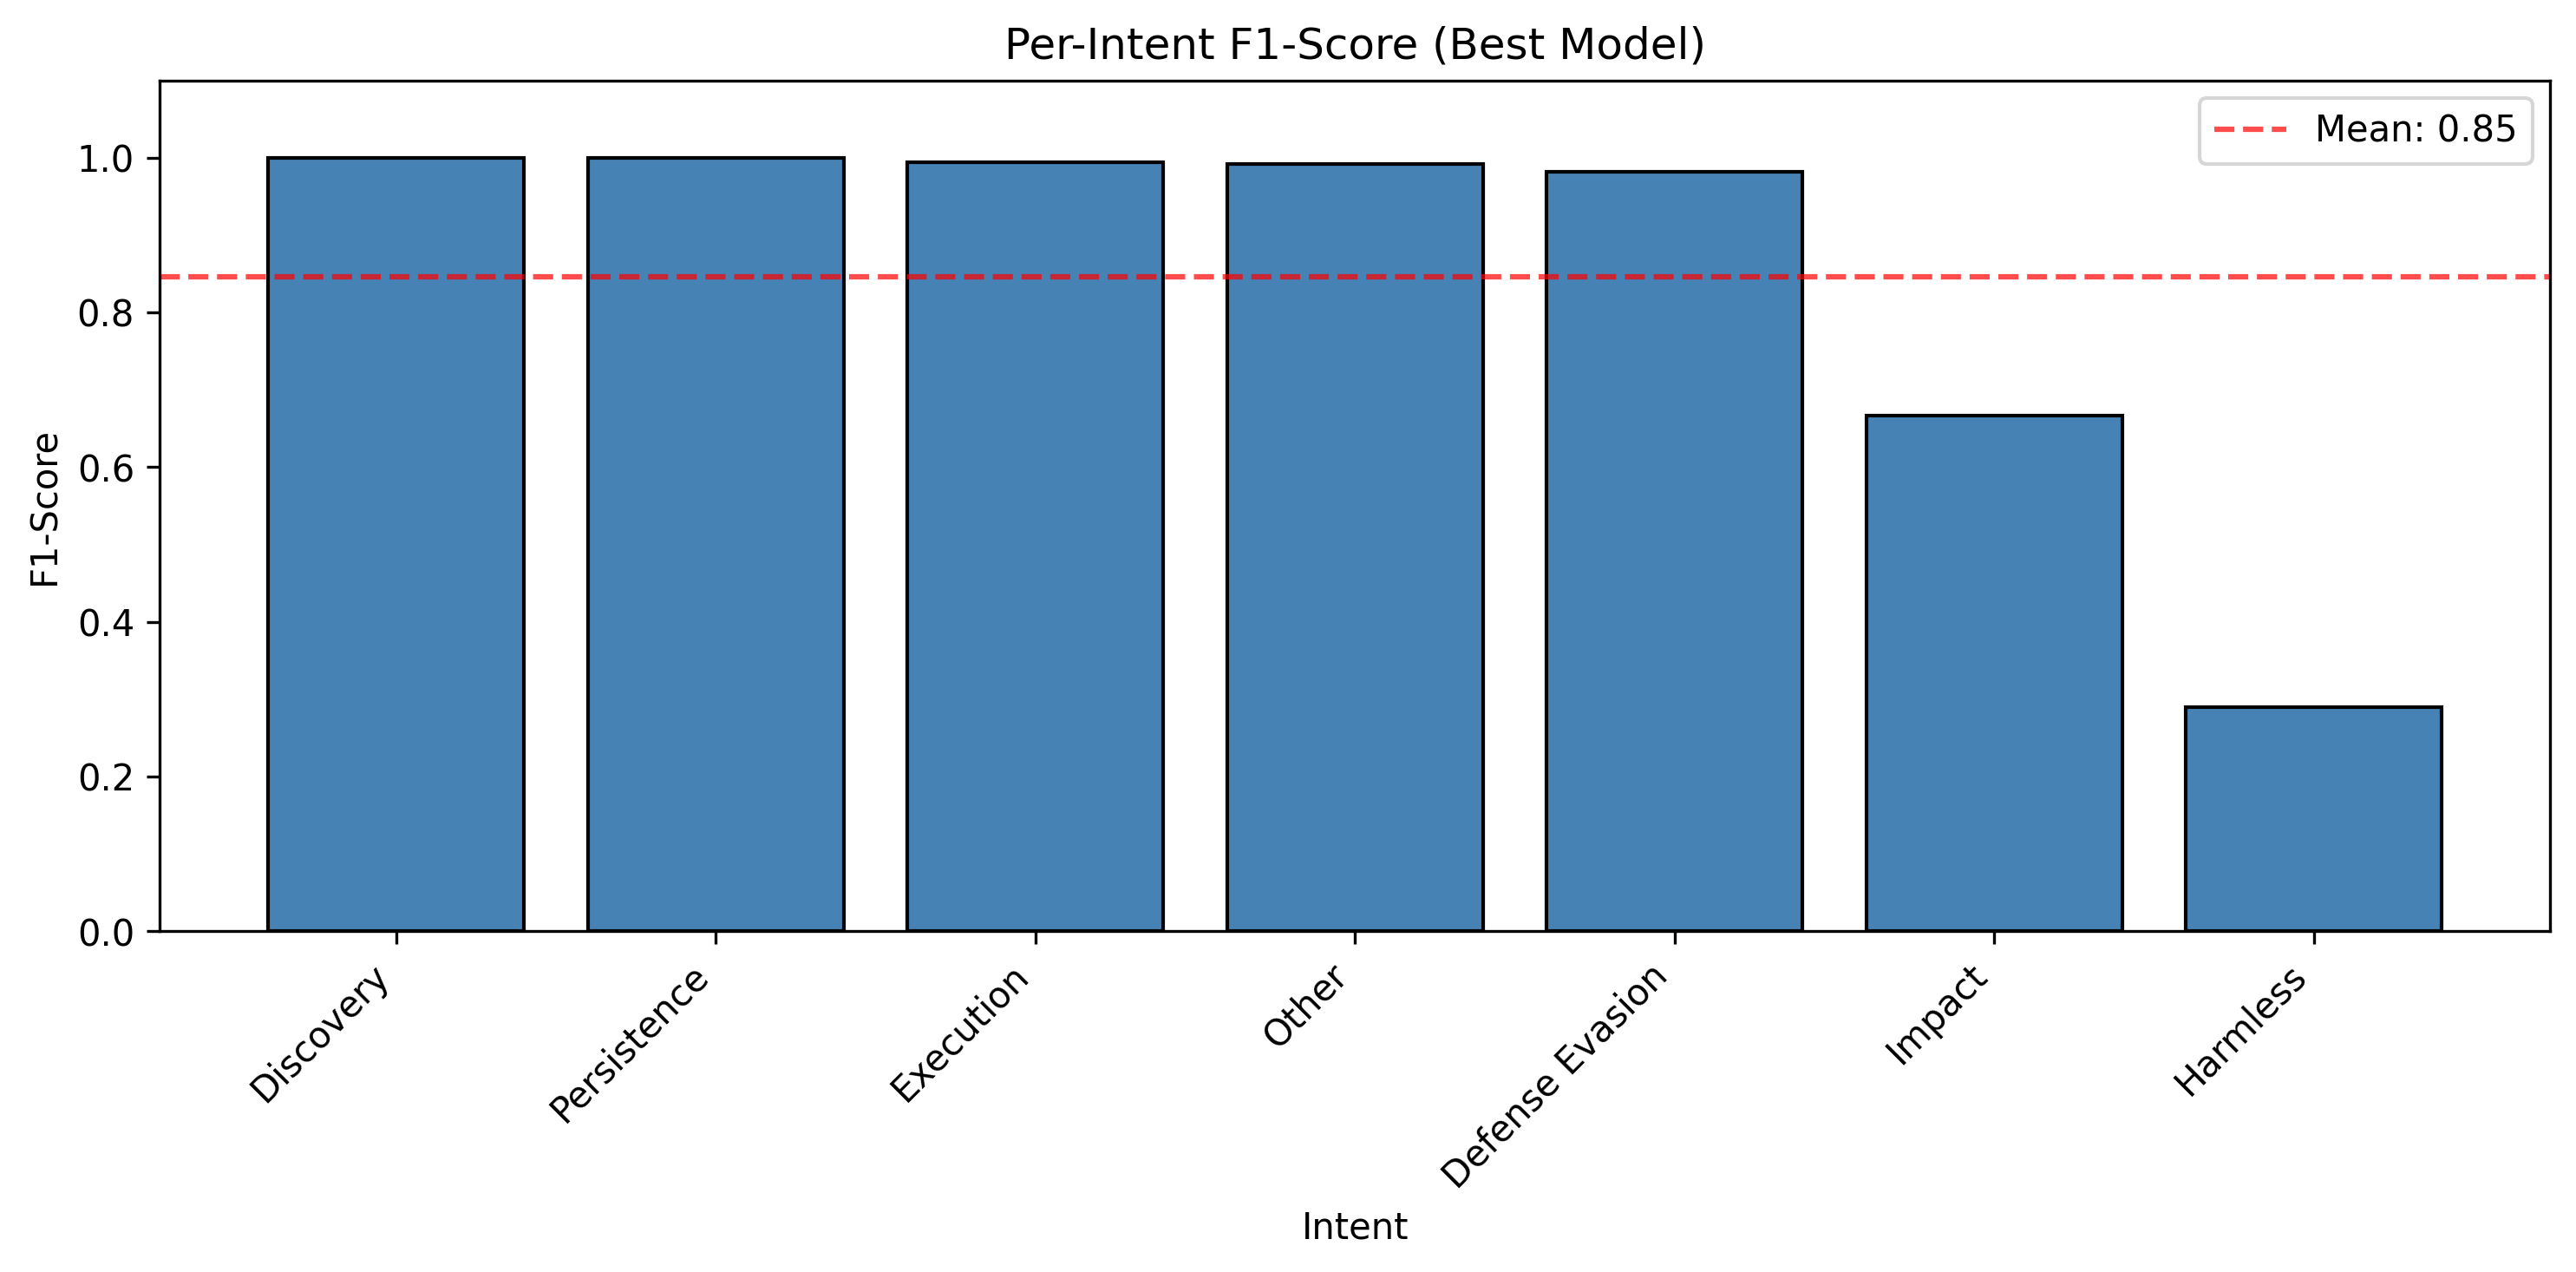
\includegraphics[width=0.6\textwidth]{results/plots/section2/per_intent_f1_scores.png}
\caption{Per-intent F1-scores for best model (tuned LR). Majors excel (>0.98); minorities lag (Harmless 0.29, Impact 0.67), highlighting imbalance effects.}
\label{fig:per_intent_f1}
\end{figure}

\FloatBarrier
\subsection{Per-Intent Performance Analysis}

Models shine on frequent intents but struggle with rares:
\begin{itemize}
    \item \textbf{Strong}: Discovery/Persistence/Execution/Other/Defense Evasion (F1 0.98-1.0, tuned LR)
    \item \textbf{Challenging}: Impact (F1 0.67, few samples); Harmless (F1 0.29, recall 0.17)
\end{itemize}

\subsection{Overfitting and Generalization Analysis}

Train/test gaps are minimal:
\begin{itemize}
    \item LR (baseline): Train F1 0.9975 vs. Test 0.9958
    \item RF (baseline): Train 0.9984 vs. Test 0.9964
    \item LR (tuned): Train 0.9975 vs. Test 0.9964 (best balance)
    \item RF (tuned): Train 0.9971 vs. Test 0.9963
\end{itemize}

Tuned LR generalizes best for imbalanced data.

\subsection{Discussion}

Tuned LR edges out with macro F1 0.8463, better suiting minorities via probabilistic weighting—proving simpler models can outperform complex ones on sparse features. Imbalance correlates with F1 (r=0.89), suggesting data augments for rares. LR's coefficients aid interpretability, revealing attack cues; future SHAP could enhance this. Overall, these models turn logs into reliable threat intel.

% ============================================
% SECTION 4: UNSUPERVISED LEARNING - CLUSTERING
% ============================================
\section{Unsupervised Learning - Clustering}

\subsection{Clustering Methodology}

Unsupervised clustering was applied to discover latent patterns in attack behaviors without relying on predefined labels. Two primary algorithms were implemented:

\paragraph{K-Means Clustering} partitions sessions into k clusters by minimizing within-cluster sum of squared distances. The algorithm iteratively:
\begin{enumerate}
    \item Assigns each session to the nearest cluster centroid
    \item Recalculates centroids as the mean of assigned sessions
    \item Repeats until convergence
\end{enumerate}

\paragraph{Agglomerative Hierarchical Clustering} builds a hierarchy of clusters using a bottom-up approach:
\begin{enumerate}
    \item Starts with each session as a singleton cluster
    \item Iteratively merges the closest pair of clusters based on Ward linkage
    \item Continues until reaching the desired number of clusters
\end{enumerate}

\subsection{Determining Optimal Number of Clusters}

Multiple evaluation metrics were used to determine the optimal $k$ for K-Means clustering, as shown in Figure~\ref{fig:kmeans_metrics}:

\begin{itemize}
    \item \textbf{Elbow Method}: Plots within-cluster sum of squares (WCSS) vs. number of clusters. The "elbow" at k=10 suggests diminishing returns beyond this point
    \item \textbf{Silhouette Score}: Measures cluster cohesion and separation. Peak at k=19 with score = 0.325, though k=10 shows strong performance at 0.309
    \item \textbf{Calinski-Harabasz Index}: Ratio of between-cluster to within-cluster dispersion. Shows consistent decline, with k=10 providing good balance (score $\approx$ 12404)
    \item \textbf{Davies-Bouldin Index}: Average similarity ratio of each cluster with its most similar cluster. Lower values preferred; local minimum at k=7 (score = 1.180) with k=10 close (score = 1.422)
\end{itemize}

Considering the convergence across metrics and the clear elbow at k=10, combined with the need for interpretable cluster granularity, \textbf{k=10} was selected as the optimal number of clusters for subsequent analysis.

\begin{figure}[htbp]
\centering
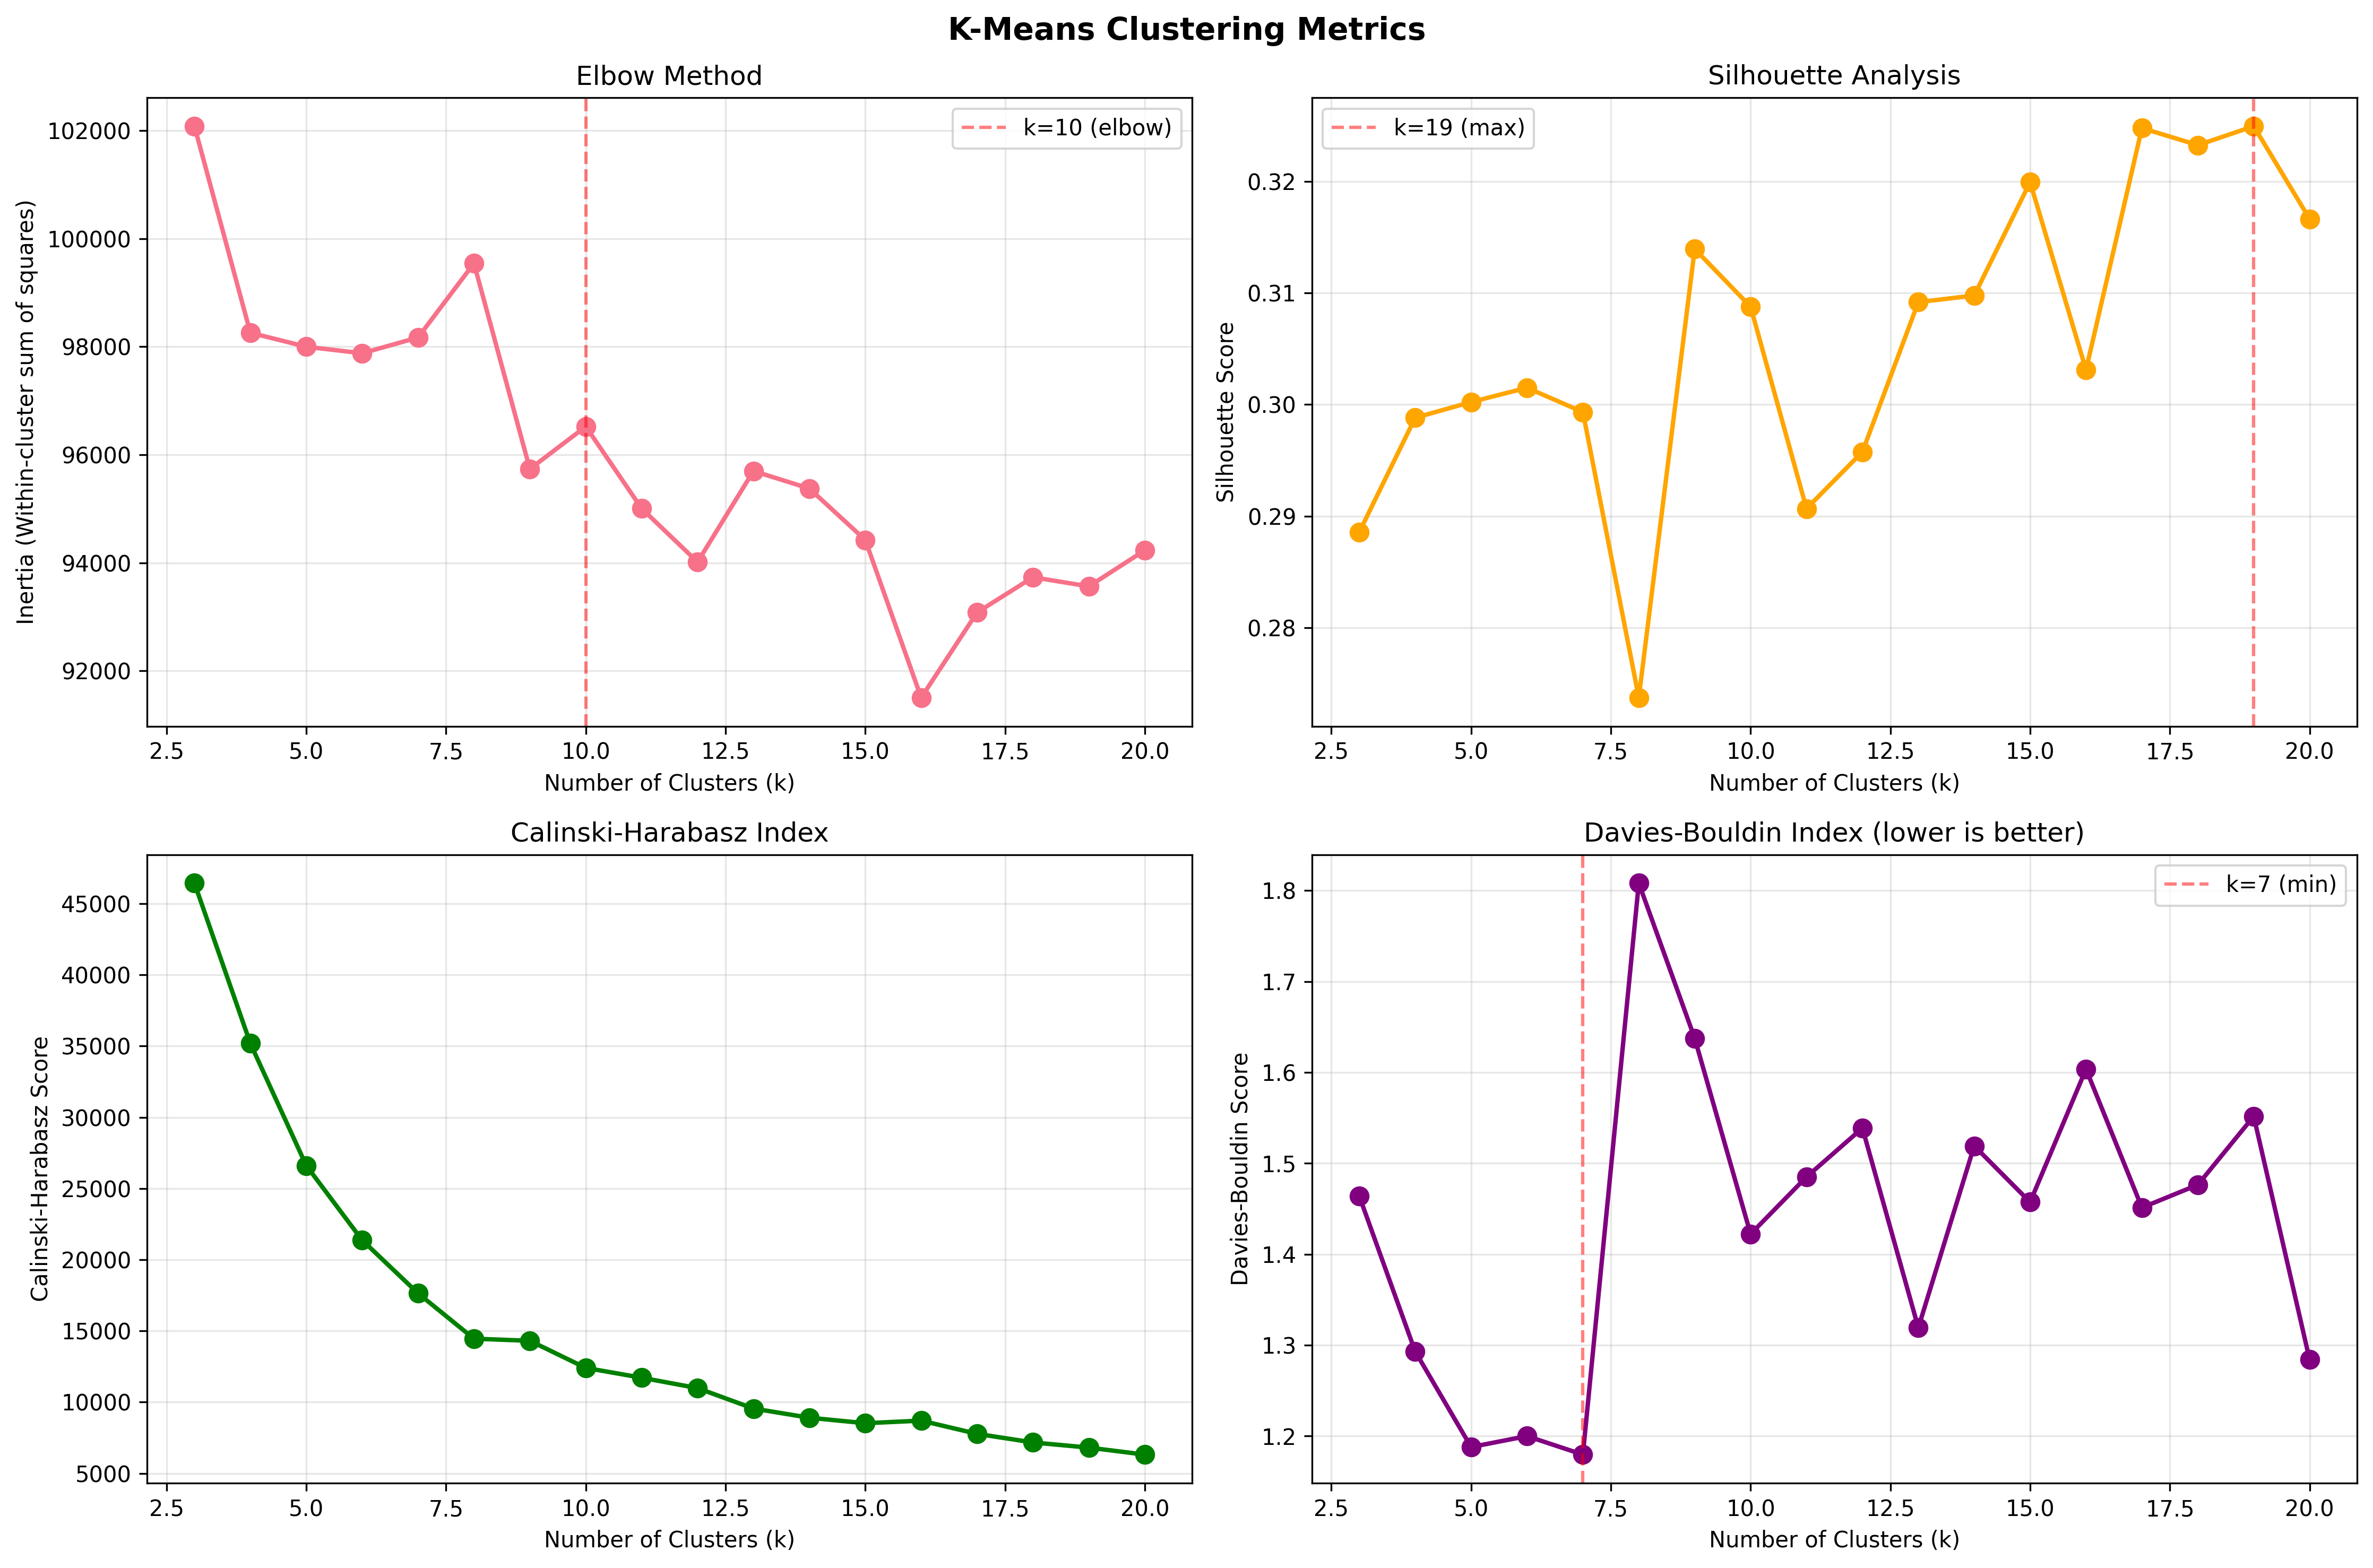
\includegraphics[width=0.80\textwidth]{results/plots/section3/kmeans_metrics.png}
\caption{K-Means evaluation metrics for determining optimal cluster count. Top-left: Elbow plot, Top-right: Silhouette score, Bottom-left: Calinski-Harabasz Index, Bottom-right: Davies-Bouldin Index. Combined evidence supports k=10 selection.}
\label{fig:kmeans_metrics}
\end{figure}

\FloatBarrier
\subsection{Cluster Validation and Algorithm Agreement}

To validate the robustness of discovered patterns, we compared K-Means clustering with Agglomerative Hierarchical Clustering using Ward linkage (Figure~\ref{fig:algorithm_comparison_appendix} in \hyperref[appendix:C2]{Appendix C.2}). The two algorithms demonstrated strong agreement:

\begin{itemize}
    \item \textbf{Adjusted Rand Index (ARI)}: 0.819, indicating high partition similarity
    \item \textbf{Normalized Mutual Information (NMI)}: 0.839, confirming consistent information capture
\end{itemize}

This high agreement validates that the discovered clusters represent genuine structural patterns in the data rather than algorithmic artifacts. Dimensionality reduction visualizations (t-SNE, UMAP) (Figure~\ref{fig:cluster_visualization_appendix} in \hyperref[appendix:C1]{Appendix C.1}) confirm reasonable cluster separation with expected overlap between semantically similar attack types. The hierarchical dendrogram (Figure~\ref{fig:hierarchical_dendrogram_appendix} in \hyperref[appendix:C2]{Appendix C.2}) suggests 8-12 clusters at a distance cut of 50, aligning with our k=10 choice.

\subsection{Cluster Characterization}

Word cloud analysis (Figure~\ref{fig:wordclouds_sample}) reveals distinctive command patterns across clusters, with session counts indicating scale:

\begin{itemize}
    \item \textbf{Cluster 0} (8 sessions): Pure reconnaissance ('var', 'proc', 'cat', 'cpuinfo', 'grep', 'uname')
    \item \textbf{Cluster 1} (84,047 sessions): Large-scale scanning ('var0352z123', 'tmp', 'cat', 'proc', 'grep', 'cpuinfo')
    \item \textbf{Cluster 2} (17,574 sessions): System manipulation ('bin', 'busybox', 'system', 'shell', 'enable', 'mounts')
    \item \textbf{Cluster 3} (2,035 sessions): Encoded payloads ('jeSjax', 'busybox', 'wget', 'chmod', 'sh')
    \item \textbf{Clusters 4-9}: Variations on discovery, execution, and persistence themes (detailed in \hyperref[appendix:C3]{Appendix C.3})
\end{itemize}

\begin{figure}[htbp]
\centering
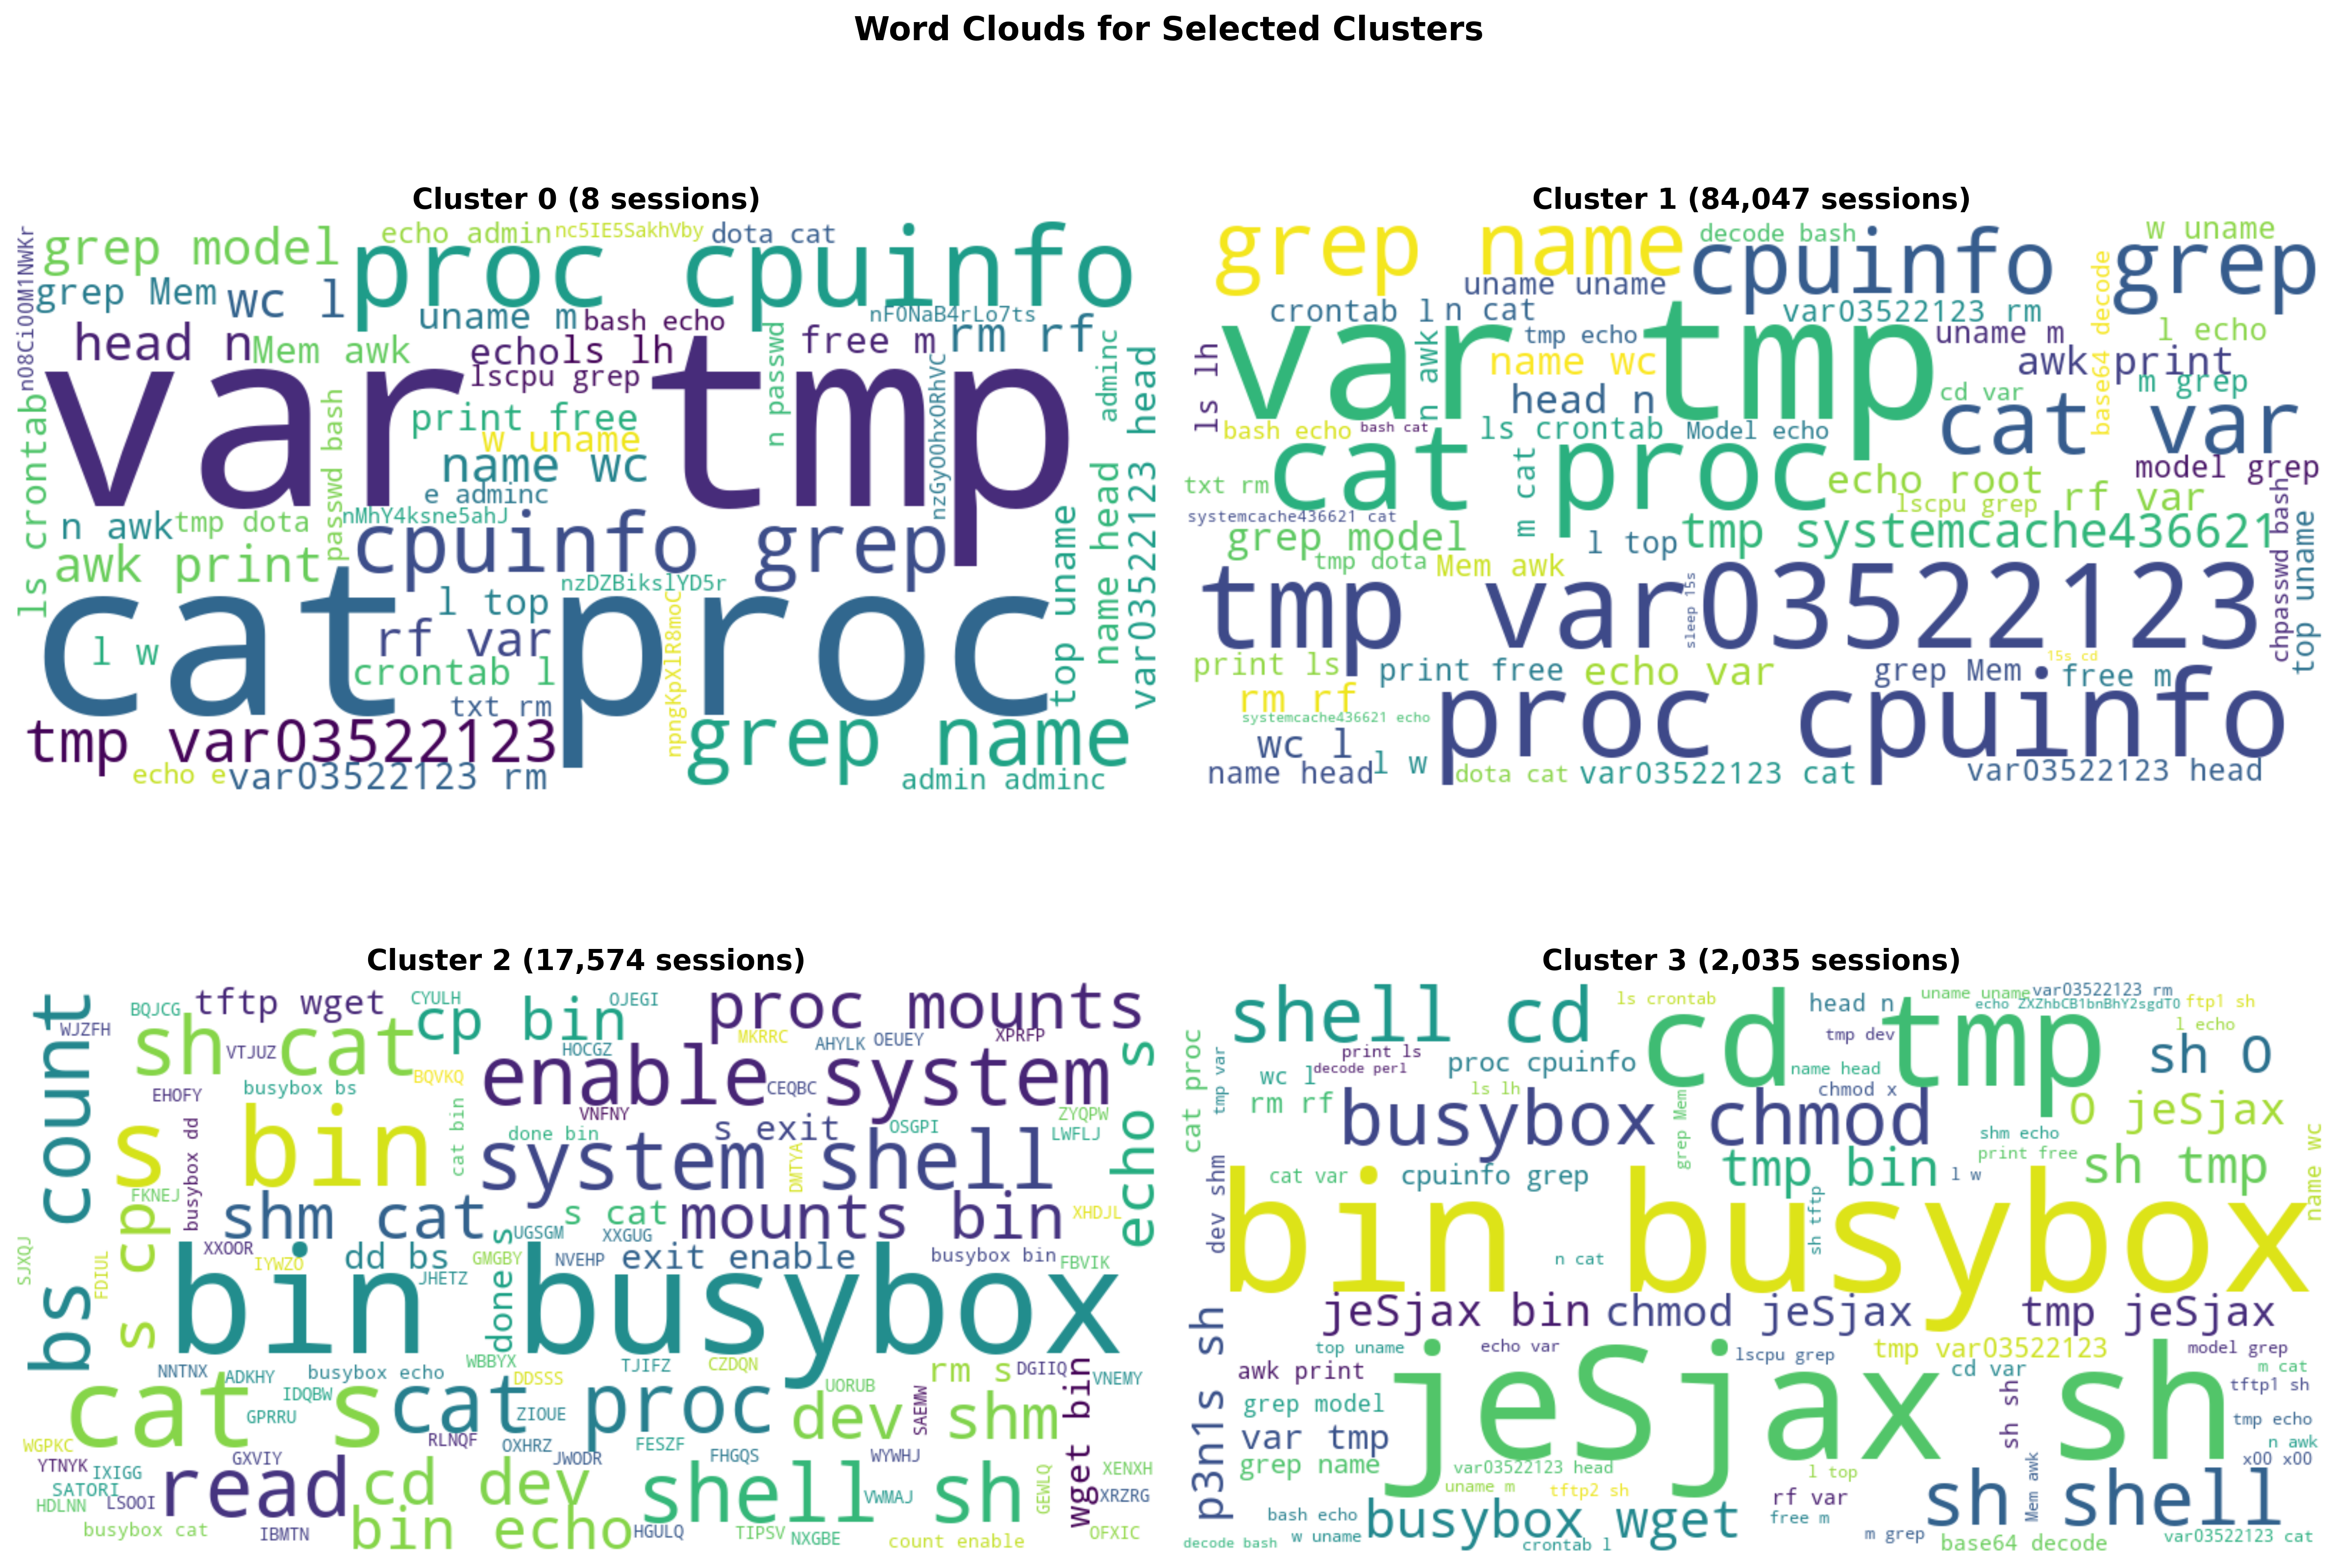
\includegraphics[width=0.75\textwidth]{results/plots/section3/cluster_wordclouds.png}
\caption{Word clouds for selected clusters showing characteristic command patterns. Font size indicates term frequency.}
\label{fig:wordclouds_sample}
\end{figure}

\FloatBarrier

\subsection{Cluster-Intent Alignment}

Figure~\ref{fig:cluster_intent_heatmap} shows cluster-intent associations. Key findings:

\begin{itemize}
    \item \textbf{Discovery Dominance}: Near 100\% association in 8 of 10 clusters (e.g., 57.6\% in Cluster 3, 96.5\% in Cluster 8), confirming reconnaissance as fundamental to SSH attacks
    \item \textbf{High-Purity Clusters}: Cluster 2 (99.3\% Defense Evasion), Cluster 9 (100\% triple: Discovery, Execution, Persistence)
    \item \textbf{Multi-Intent Sophistication}: Cluster 8 exhibits balanced multi-tactic behavior (96.5\% Defense Evasion/Discovery, 97.7\% Execution, 61.6\% Persistence)
\end{itemize}

The stacked bar chart (Figure~\ref{fig:intent_composition_stacked} in \hyperref[appendix:C4]{Appendix C.4}) further illustrates multi-label intent distributions per cluster.

\begin{figure}[htbp]
\centering
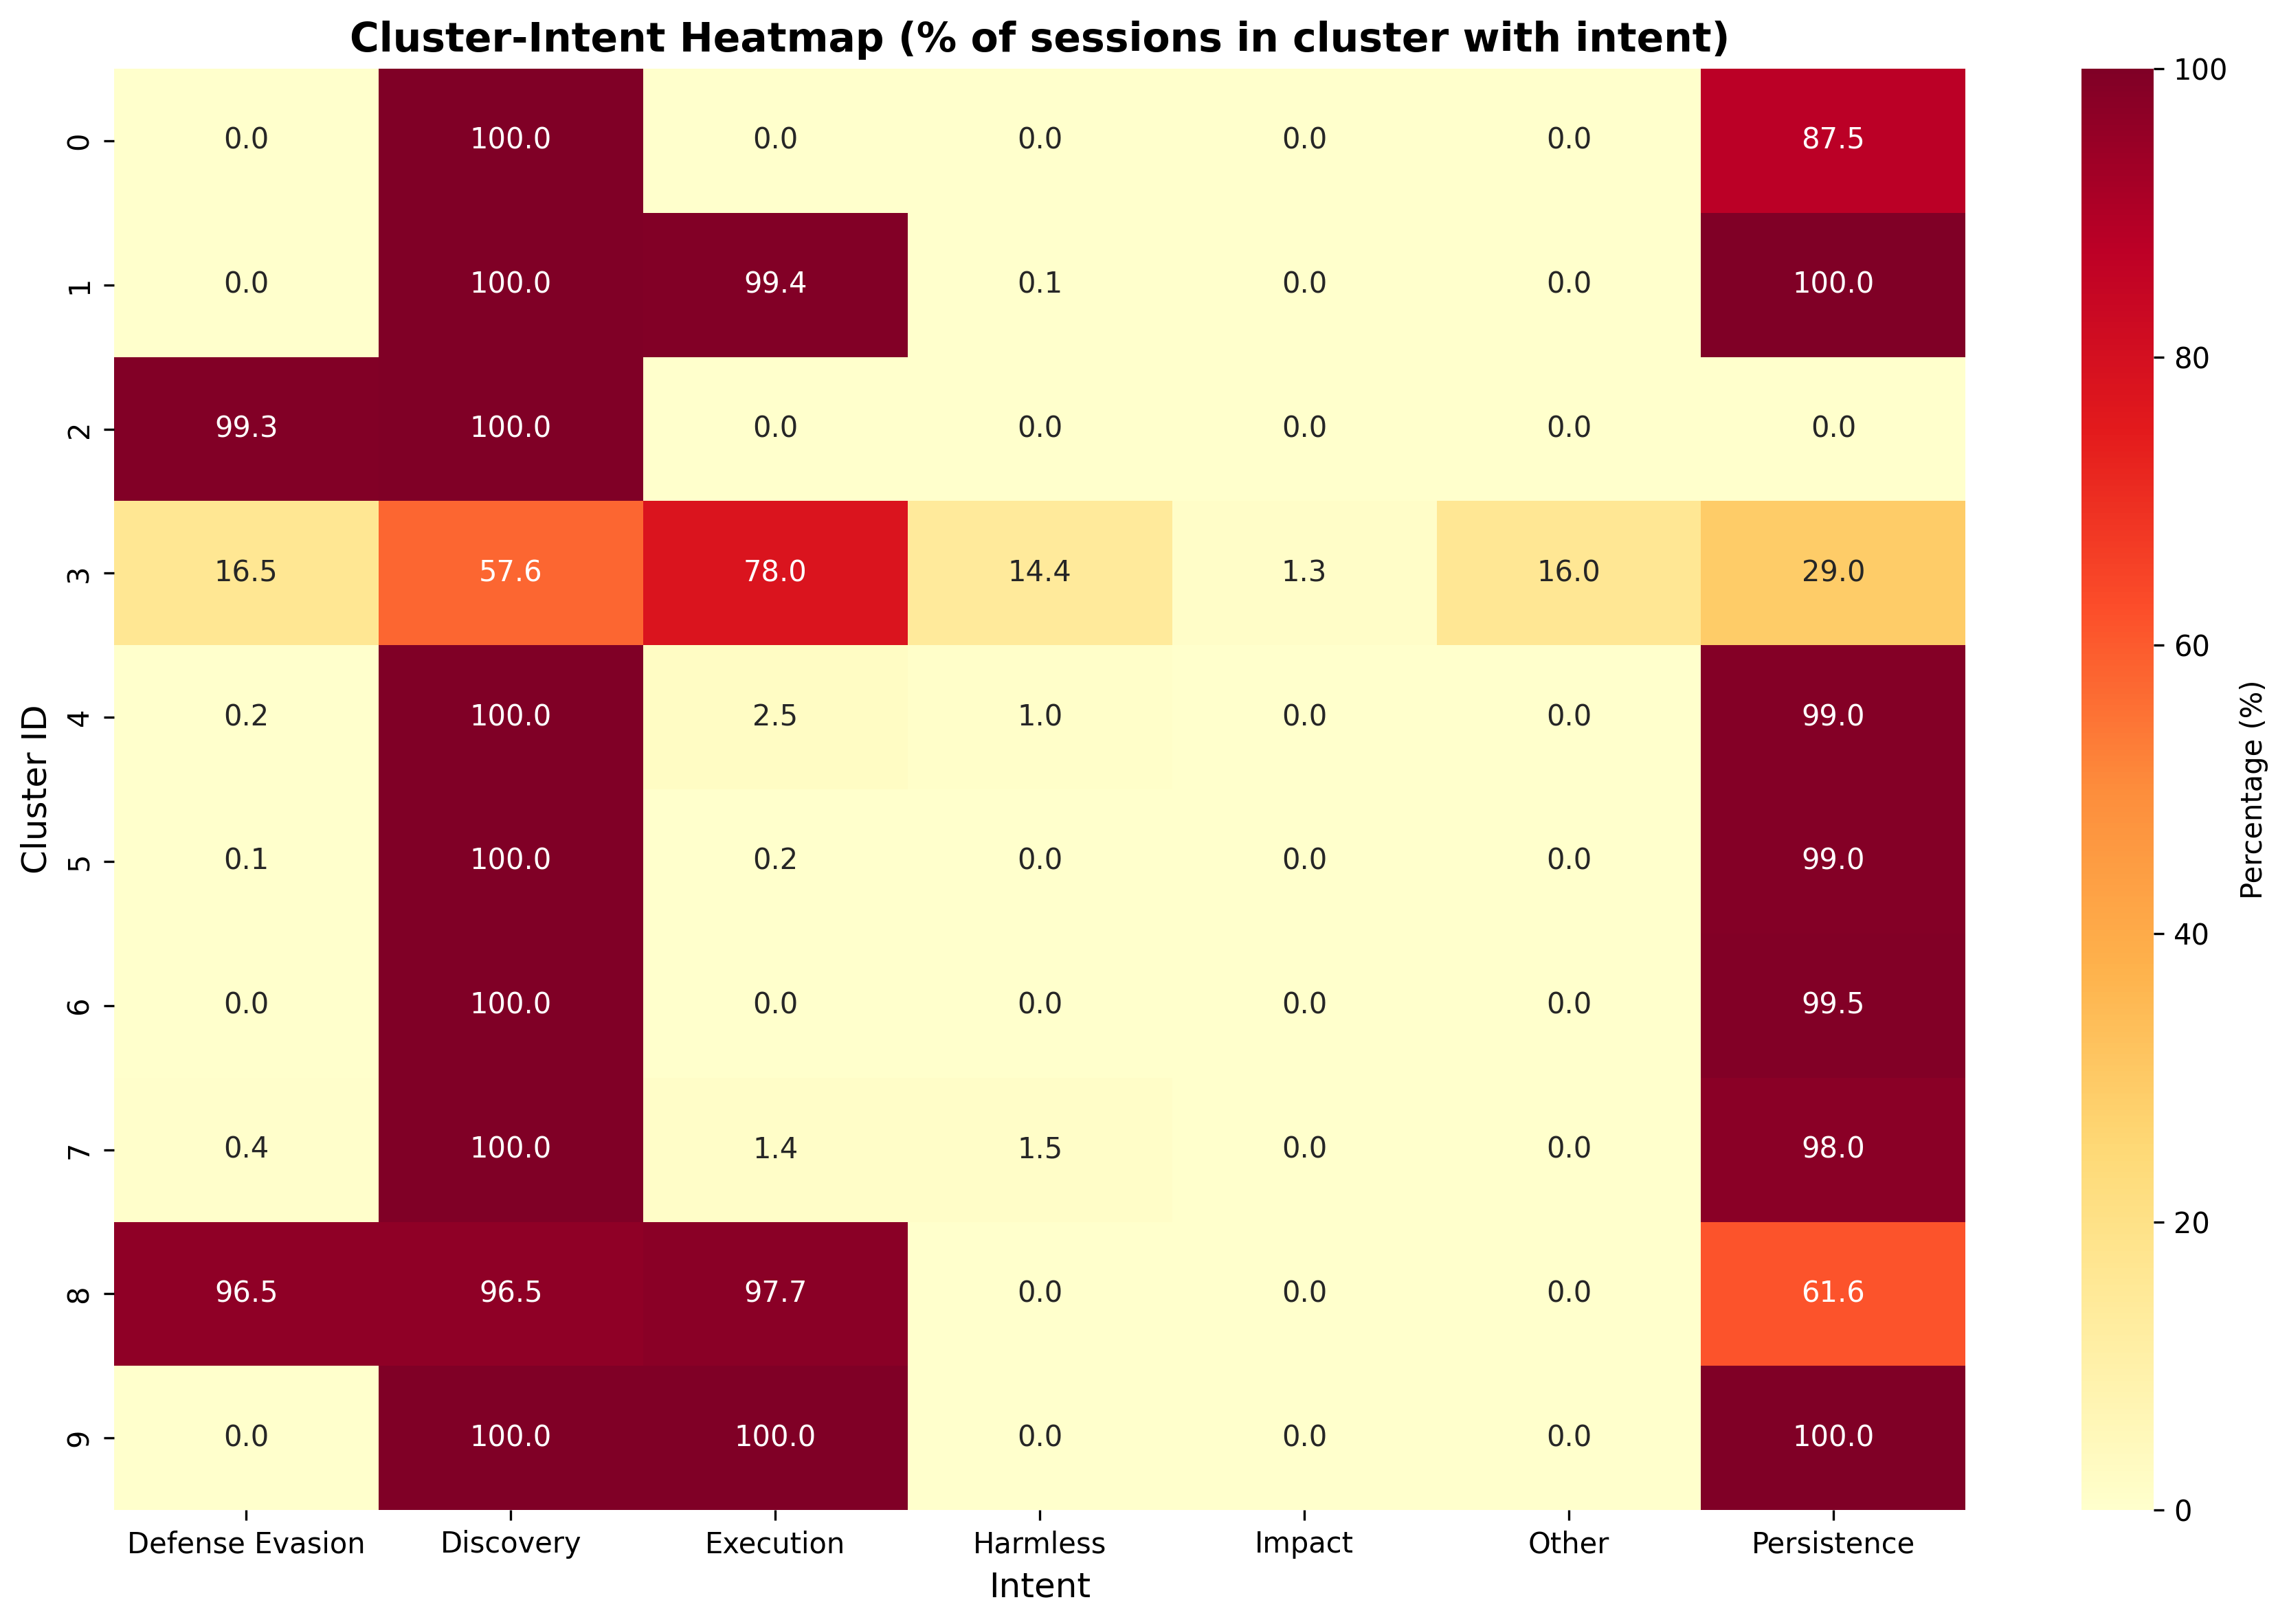
\includegraphics[width=0.7\textwidth]{results/plots/section3/cluster_intent_heatmap.png}
\caption{Cluster-intent association heatmap showing strong alignment between unsupervised clusters and MITRE ATT\&CK intents.}
\label{fig:cluster_intent_heatmap}
\end{figure}

\FloatBarrier

\subsection{Cluster Purity and Characterization}

Figure~\ref{fig:cluster_purity} shows purity scores for all 10 clusters. Nine clusters achieve $\geq$95\% purity, with weighted average of 97.75\%, indicating highly homogeneous intent-based grouping. Cluster characteristics (detailed in \hyperref[appendix:C3]{Appendix C.3}):

\begin{itemize}
    \item \textbf{Clusters 0, 4-7}: Persistence-dominated (87-99\% purity)
    \item \textbf{Clusters 1, 3, 8-9}: Execution-dominated (78-100\% purity)
    \item \textbf{Cluster 2}: Defense Evasion-dominated (99\% purity)
\end{itemize}

\begin{figure}[htbp]
\centering
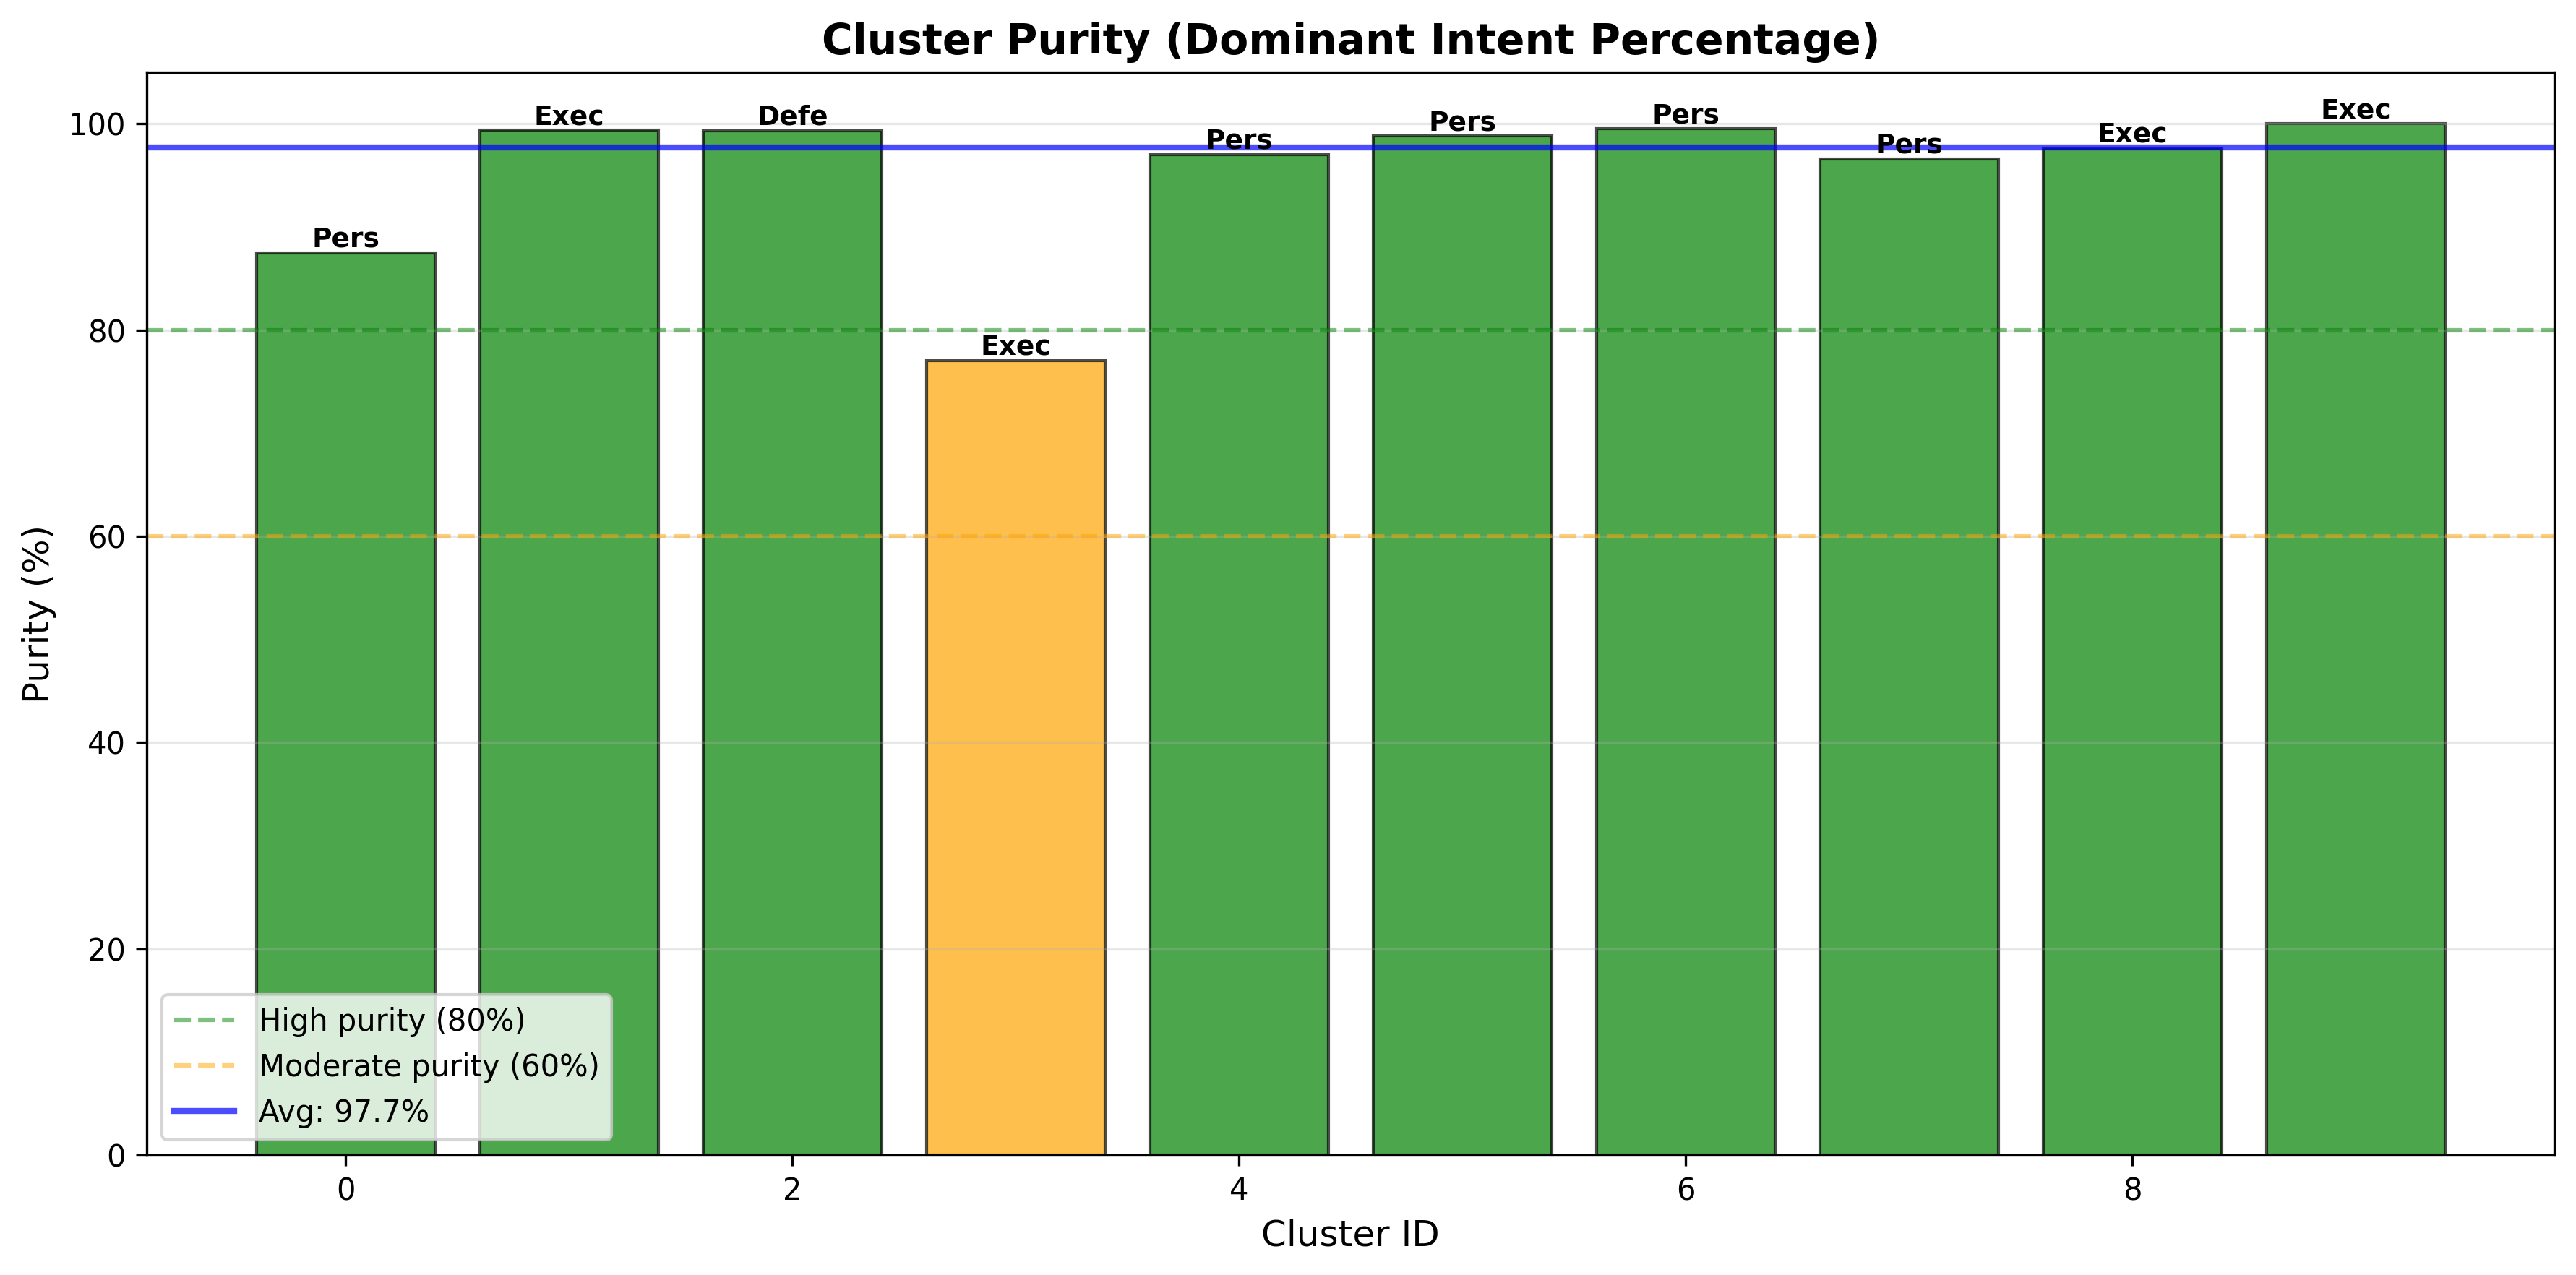
\includegraphics[width=0.7\textwidth]{results/plots/section3/cluster_purity.png}
\caption{Cluster purity scores showing 9 of 10 clusters achieve >95\% purity (weighted average: 97.75\%).}
\label{fig:cluster_purity}
\end{figure}

\FloatBarrier

\subsection{Attack Category Taxonomy}

Synthesizing cluster characteristics and session volumes, four primary attack categories emerged (Figure~\ref{fig:attack_categories}):

\begin{enumerate}
    \item \textbf{System Reconnaissance} (6 clusters, ~200,000 sessions): Automated enumeration focused on Discovery and Persistence, representing opportunistic scanning
    
    \item \textbf{Encoded Payload Execution} (2 clusters, ~25,000 sessions): Obfuscated commands with strong Execution association (78-98\%)
    
    \item \textbf{Malware Download \& Execution} (1 cluster, ~5,000 sessions): Payload retrieval and deployment with Execution and Persistence focus
    
    \item \textbf{Execution - Mixed} (1 cluster, ~5,000 sessions): Sophisticated multi-tactic attacks combining 3-4 intents simultaneously, indicating APT characteristics
\end{enumerate}

\begin{figure}[htbp]
\centering
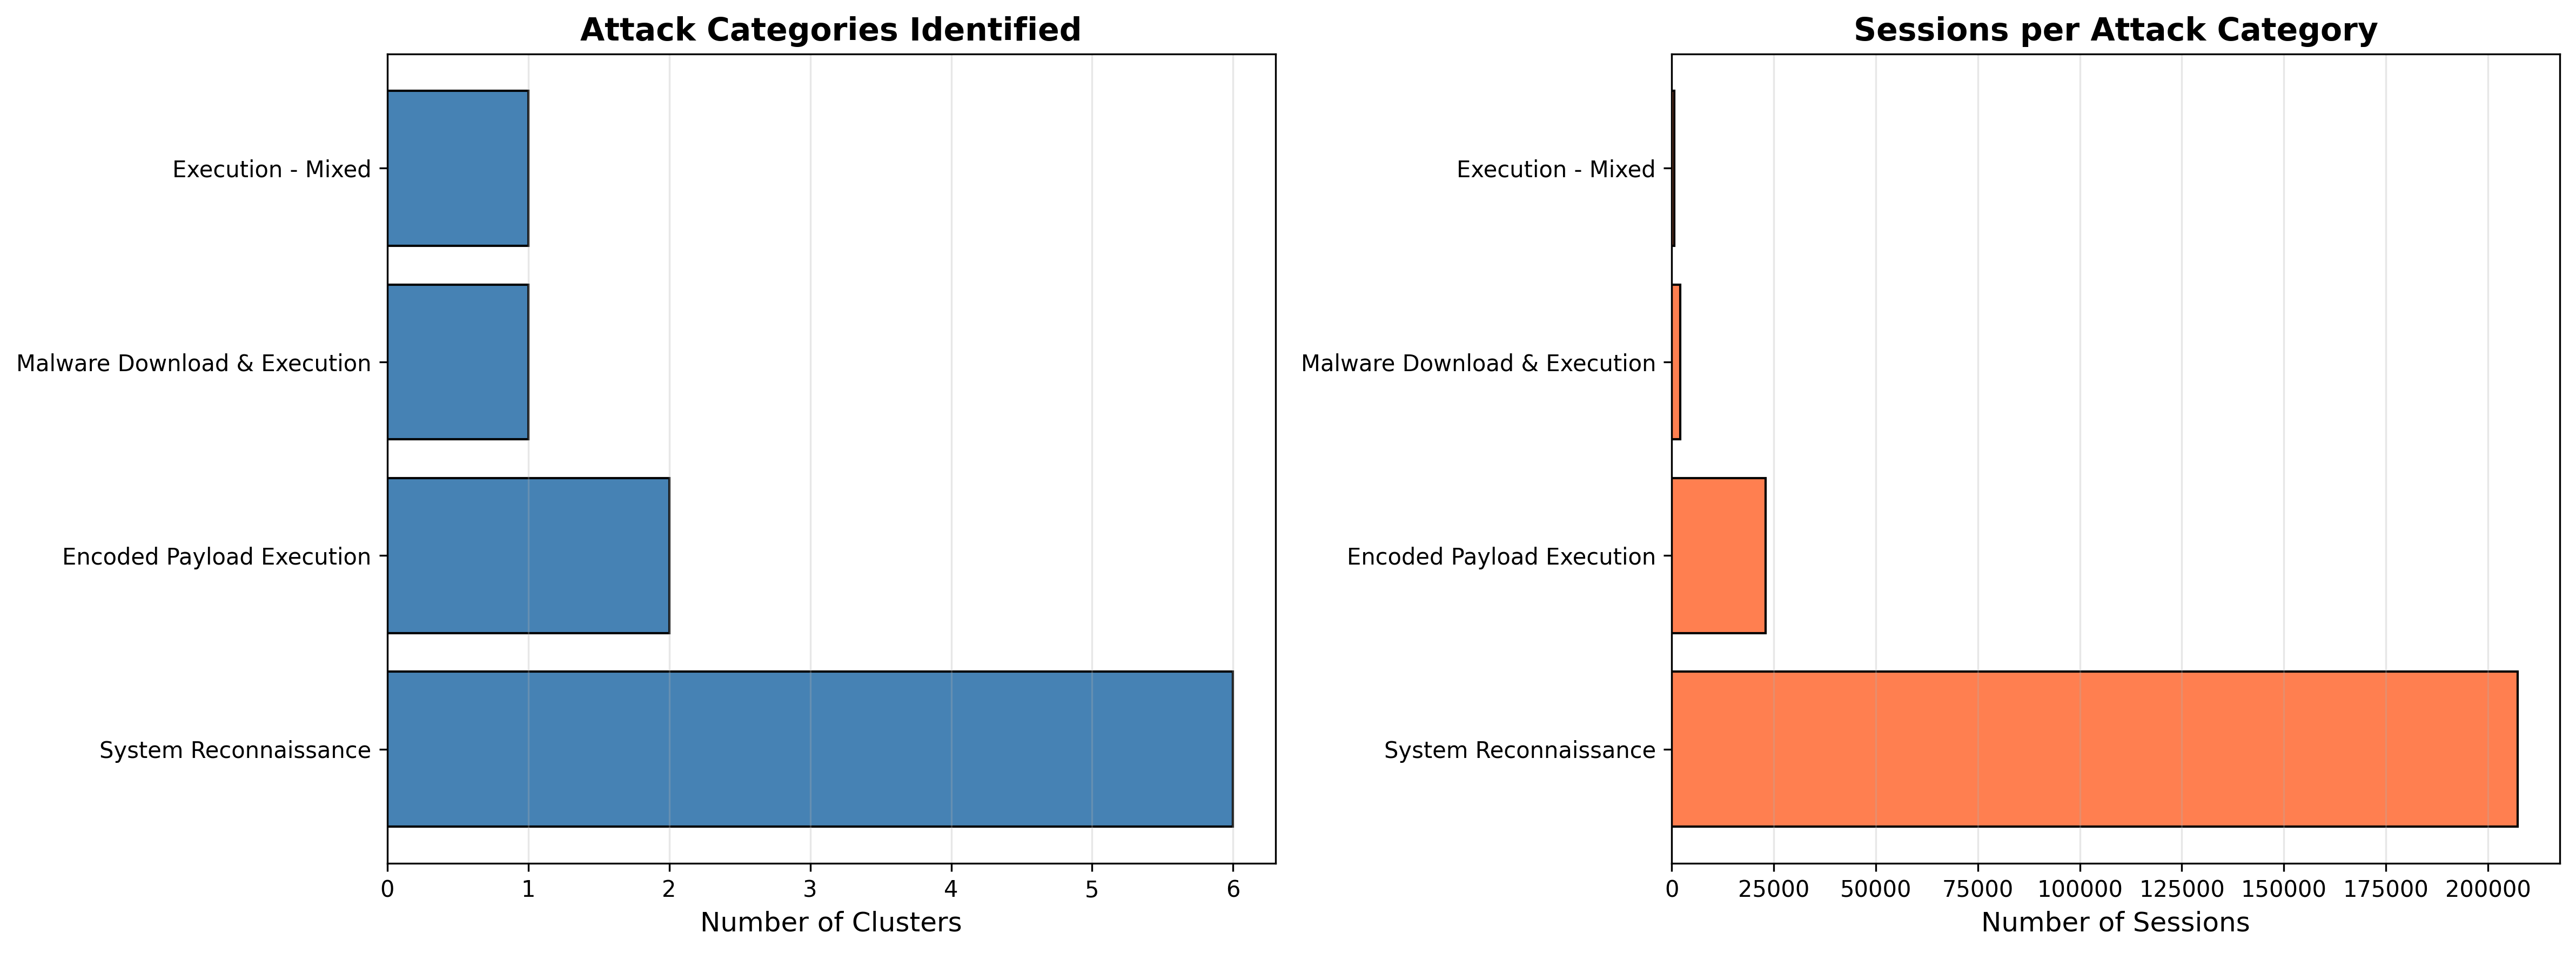
\includegraphics[width=0.85\textwidth]{results/plots/section3/attack_categories.png}
\caption{Attack category taxonomy showing System Reconnaissance dominates (200K+ sessions, 6 clusters) while specialized attacks represent 15-20\% of traffic.}
\label{fig:attack_categories}
\end{figure}

\FloatBarrier

\subsection{Discussion}

The 97.75\% weighted average purity and strong algorithm agreement (ARI=0.82, NMI=0.84) demonstrate successful discovery of homogeneous attack patterns. The remarkable alignment with MITRE ATT\&CK validates the framework's natural capture of attack behavior boundaries. The moderate Silhouette score (0.31) reflects expected overlap due to multi-label intents rather than clustering issues.

\paragraph{Operational Insights}
Clustering reveals actionable patterns beyond intent labels:
\begin{itemize}
    \item \textbf{Volume-based Risk}: 200,000+ reconnaissance sessions vs. 5,000 sophisticated multi-stage attacks enables prioritization
    \item \textbf{Signature Detection}: Distinctive command patterns (e.g., 'busybox'+'chmod' in Cluster 3) provide IDS signatures
    \item \textbf{Attack Progression}: Detecting transitions from reconnaissance (Clusters 0-1) to multi-stage attacks (Clusters 8-9) could trigger escalated alerts
    \item \textbf{Anomaly Detection}: Sessions not fitting established clusters may indicate novel techniques
\end{itemize}

This unsupervised approach complements supervised classification by revealing operational attack patterns not fully captured by intent labels alone.

% ============================================
% SECTION 5: LANGUAGE MODELS - BERT FINE-TUNING
% ============================================
\section{Language Model Exploration - BERT Fine-Tuning}

\subsection{Model Selection and Architecture}

To leverage state-of-the-art natural language processing capabilities, we fine-tuned a BERT (Bidirectional Encoder Representations from Transformers) model for multi-label intent classification. The architecture consists of:

\begin{itemize}
    \item \textbf{Base Model}: \texttt{bert-base-uncased} pre-trained on large text corpora
    \item \textbf{Classification Head}: Custom dense layer with sigmoid activation for multi-label output
    \item \textbf{Input Representation}: Tokenized attack sessions with [CLS] token for classification
    \item \textbf{Maximum Sequence Length}: 256 tokens, with truncation or padding applied as needed, to balance information retention and computational efficiency
\end{itemize}

\textbf{Justification for BERT over Doc2Vec}:
\begin{itemize}
    \item BERT captures bidirectional context, crucial for understanding command sequences
    \item Pre-training on large corpora provides robust general-language understanding
    \item Fine-tuning enables effective adaptation to the cybersecurity domain
    \item The transformer architecture handles variable-length input sequences effectively
\end{itemize}

\subsection{Training Configuration}

The model was trained with the following hyperparameters:

\begin{itemize}
    \item \textbf{Optimizer}: AdamW with weight decay = 0.01
    \item \textbf{Learning Rate}: $2 \times 10^{-5}$ with linear warmup
    \item \textbf{Learning Rate Scheduler}: Linear decay after warmup
    \item \textbf{Batch Size}: 32 (limited by GPU memory)
    \item \textbf{Epochs}: 3 (chosen to reduce overfitting)
    \item \textbf{Loss Function}: Binary Cross-Entropy with Logits, class-weighted to handle imbalance
    \item \textbf{Gradient Clipping}: Maximum norm = 1.0
\end{itemize}

\subsection{Training Dynamics Analysis}

Figure~\ref{fig:loss_curve} shows the BERT training progression across three epochs. Training loss decreases sharply from 0.0518 in the first epoch to 0.0113 by the third epoch, demonstrating effective learning, while validation loss remains low and stable, starting at 0.0151 and ending at 0.0119, with both converging by epoch 2.

\begin{figure}[htbp]
\centering
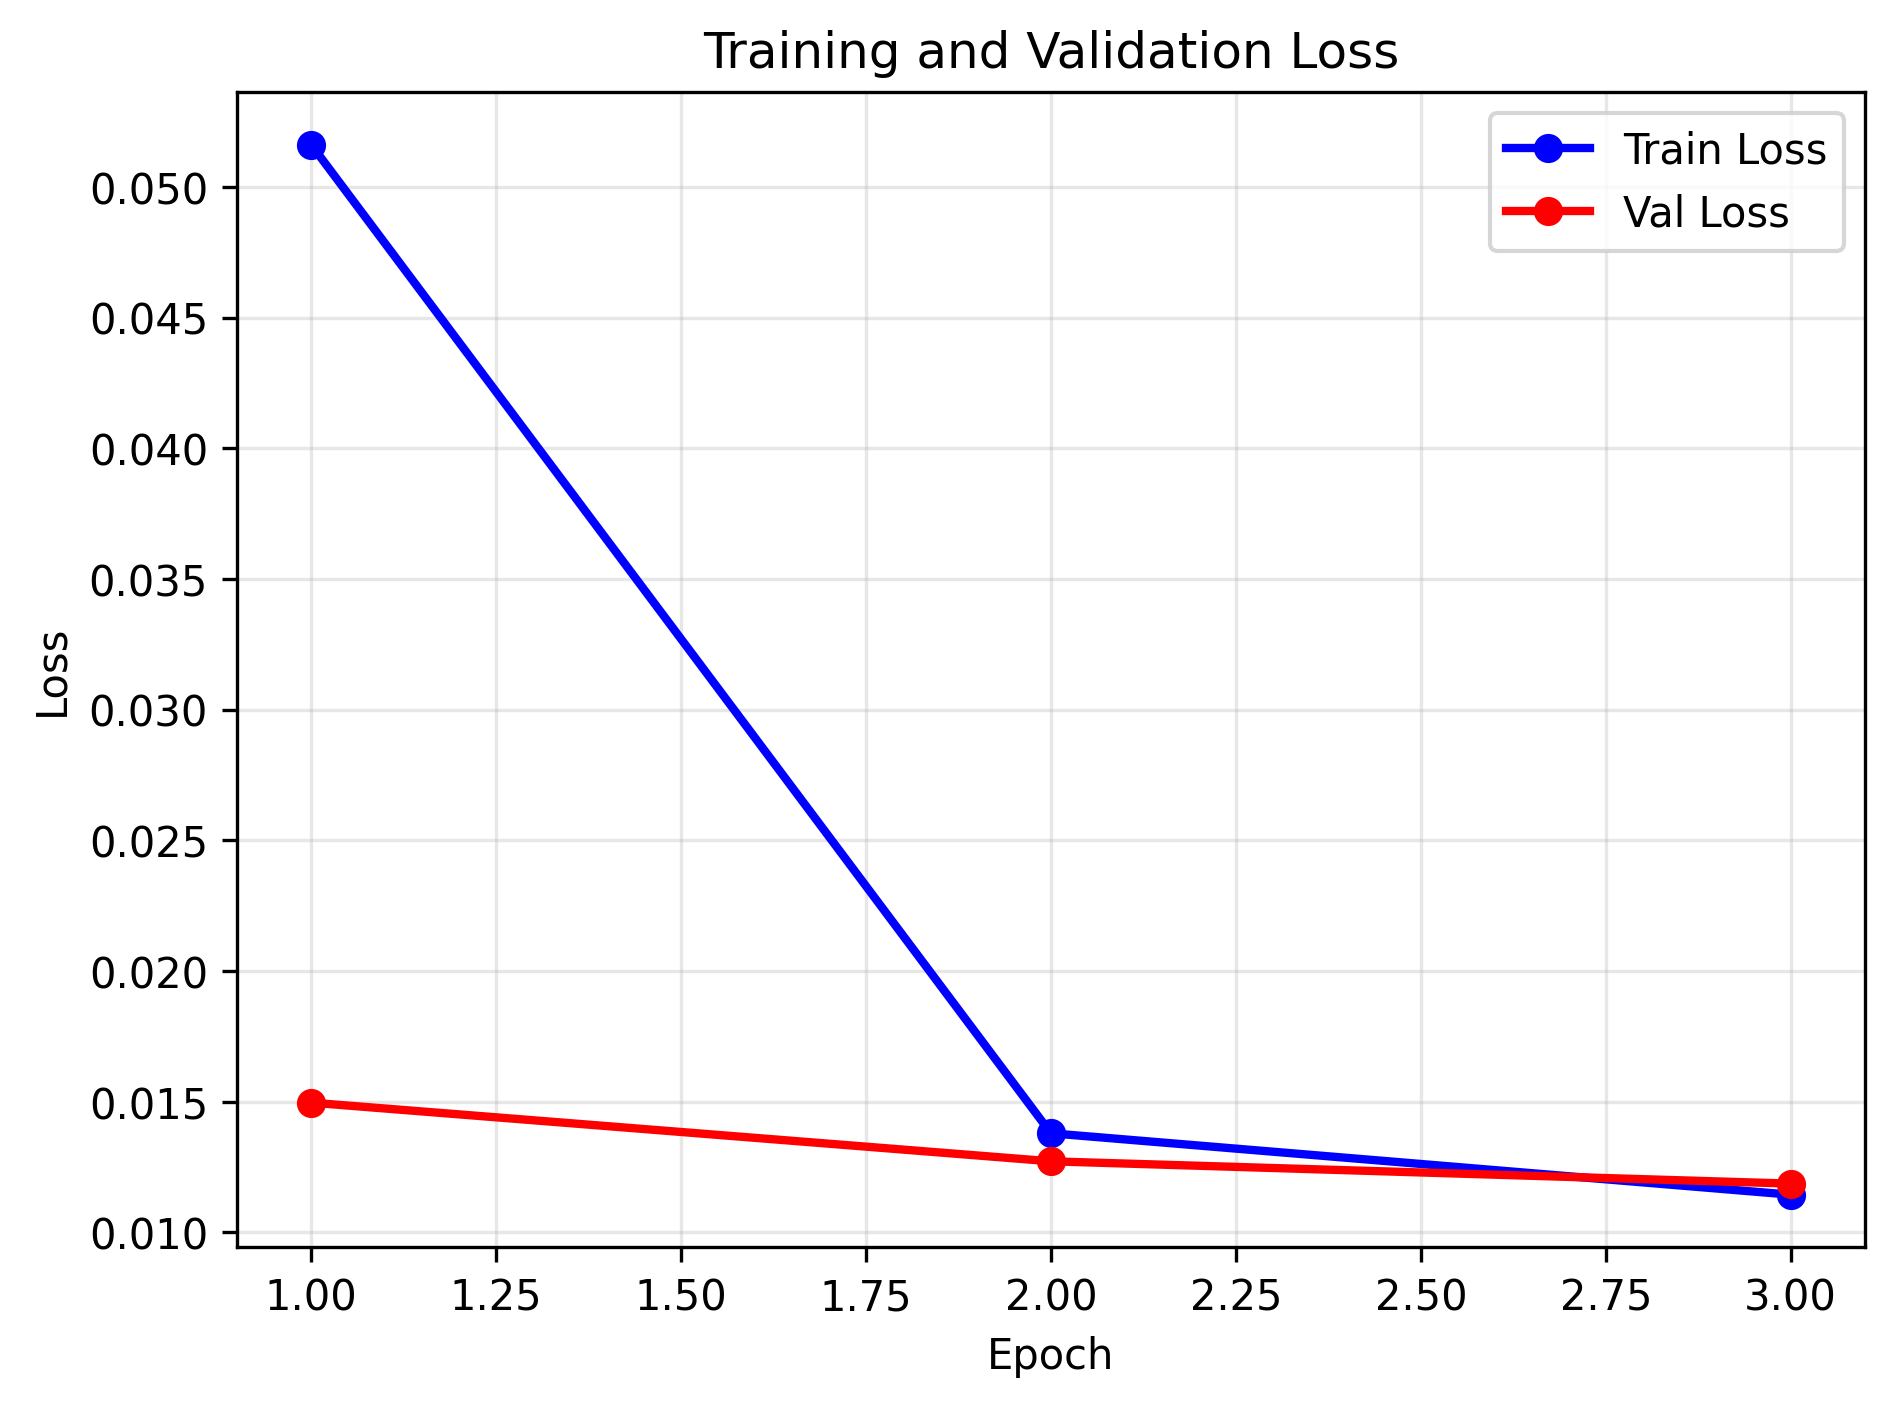
\includegraphics[width=0.7\textwidth]{results/plots/section4/loss_curve.png}
\caption{Training and validation loss curves over 3 epochs. Both curves show steady convergence with a small gap, indicating effective learning with minimal overfitting.}
\label{fig:loss_curve}
\end{figure}

The small gap between training and validation loss (0.0006 at epoch 3) indicates minimal overfitting, suggesting that the model generalizes well to unseen data. The rapid convergence reflects effective transfer learning from the pre-trained BERT weights.

Performance metrics (Figure~\ref{fig:f1_scores}) demonstrate strong model capability, with micro F1-score maintaining near-perfect performance (>0.99) across all epochs, while macro F1-score improves from 0.7253 to 0.7544, indicating better handling of minority classes despite their extreme imbalance.

\begin{figure}[htbp]
\centering
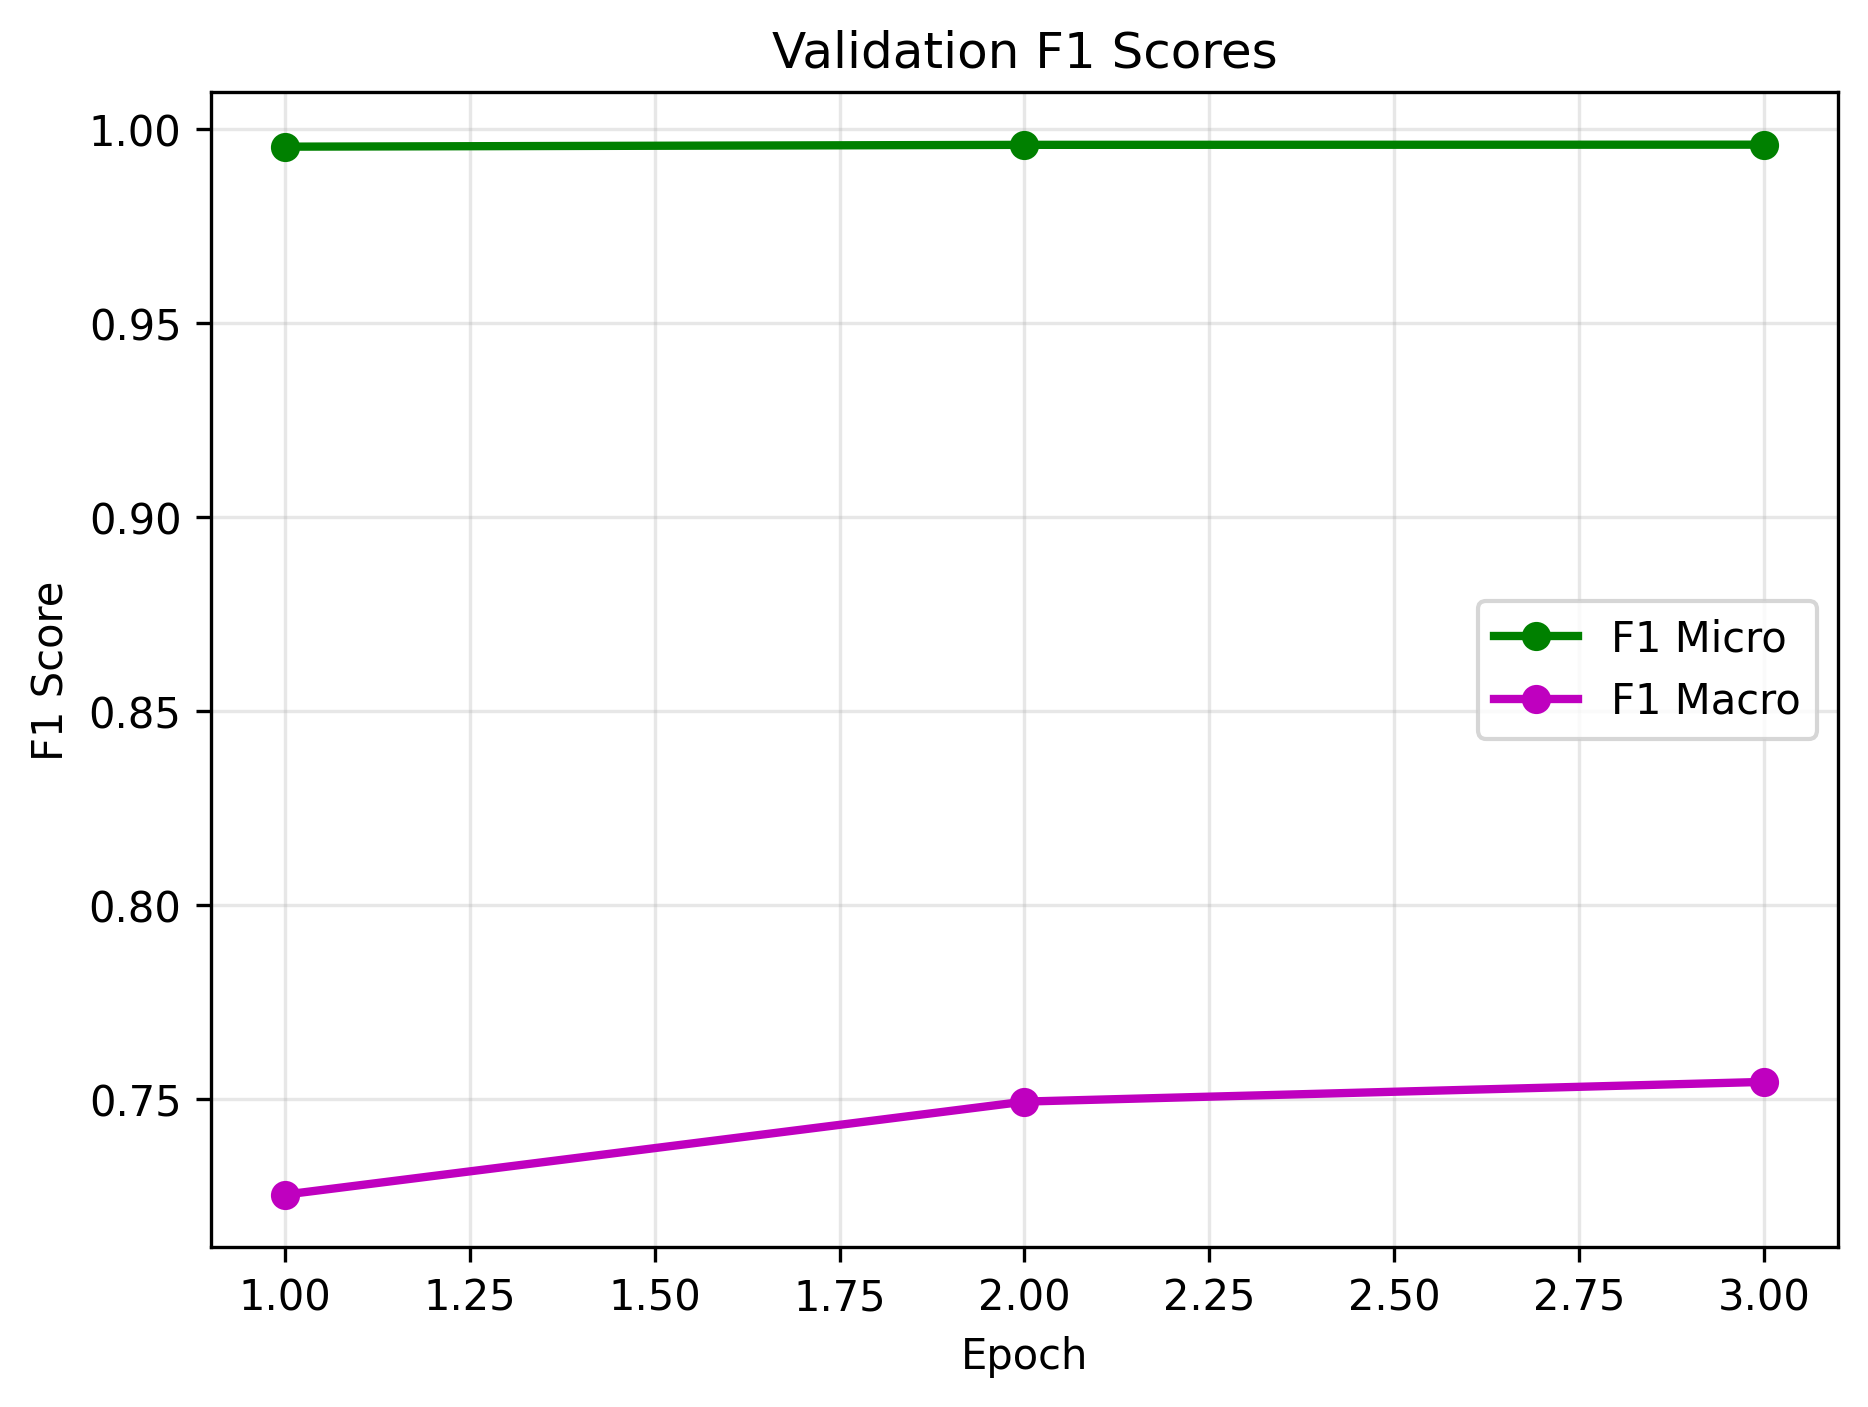
\includegraphics[width=0.7\textwidth]{results/plots/section4/f1_scores.png}
\caption{Validation F1-scores over training. High micro F1 indicates overall accuracy while improving macro F1 shows better minority class performance.}
\label{fig:f1_scores}
\end{figure}

The rapid convergence and stable validation metrics reflect effective transfer learning from pre-trained BERT weights, with class-weighted Binary Cross-Entropy successfully addressing the imbalanced dataset. The plateau of validation performance after epoch 2 confirms that 3 epochs were optimal, balancing thorough fine-tuning with computational efficiency while avoiding overfitting. 

Additional training dynamics visualizations are provided in \hyperref[appendix:D1]{Appendix D.1}.

\FloatBarrier
\subsection{Final Model Evaluation}

The final BERT model achieves strong overall performance on the test set as we can see from Table~\ref{tab:bert_results}:

\begin{table}[h]
\centering
\caption{BERT model performance on test set}
\label{tab:bert_results}
\begin{tabular}{@{}lc@{}}
\toprule
\textbf{Metric} & \textbf{Score} \\
\midrule
Test Loss & 0.0121 \\
Test Accuracy & 0.9816 \\
Hamming Loss & 0.0028 \\
F1-Score (Micro) & 0.9959 \\
F1-Score (Macro) & 0.7574 \\
\bottomrule
\end{tabular}
\end{table}


\textbf{Class Imbalance Impact:} Figure~\ref{fig:sample_dist} shows the test set distribution, with Discovery (46,433 samples, 99.6\%) and Persistence (42,281 samples, 90.7\%) dominating the dataset, while Impact (2 samples, 0.004\%), Other (67 samples, 0.14\%), and Harmless (458 samples, 0.98\%) represent less than 1\% each. This extreme imbalance significantly impacts per-intent performance despite class-weighted training.

\begin{figure}[htbp]
\centering
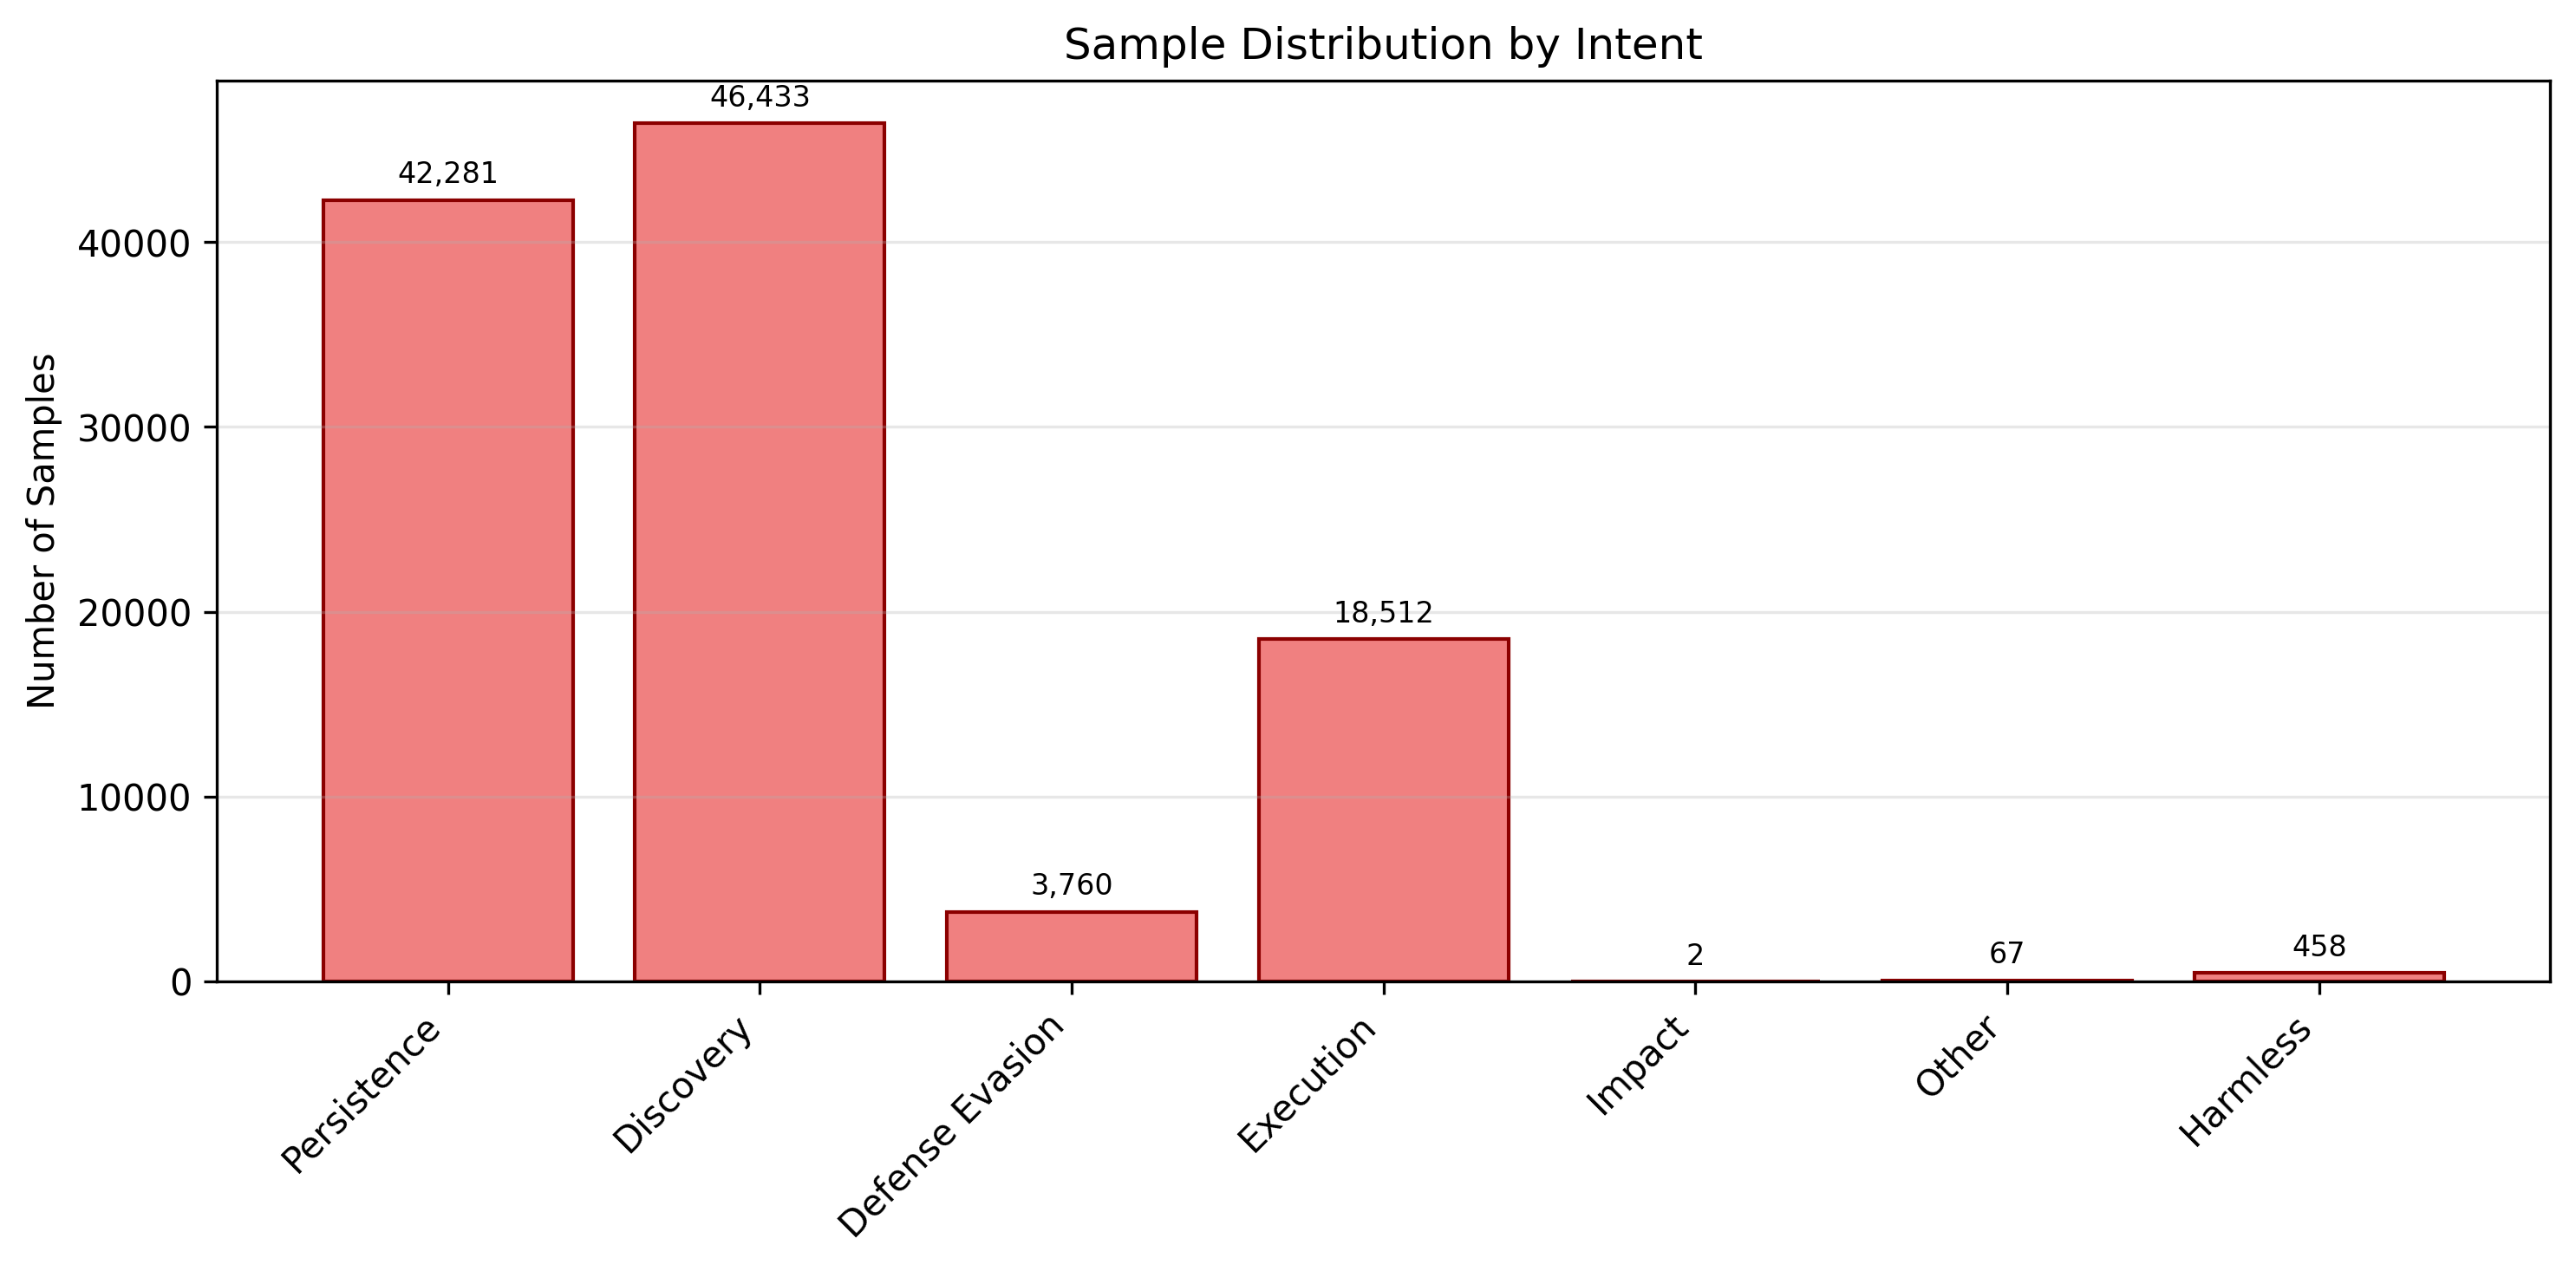
\includegraphics[width=0.7\textwidth]{results/plots/section4/sample_distribution.png}
\caption{Test set distribution across 7 intent categories showing severe class imbalance.}
\label{fig:sample_dist}
\end{figure}

\FloatBarrier
\textbf{Per-Intent Performance Analysis:} Figure~\ref{fig:f1_by_intent} reveals the direct consequence of class imbalance on model performance. Majority classes achieve near-perfect F1-scores: Discovery (F1: 0.9999), Persistence (F1: 0.9995), Execution (F1: 0.991), and Defense Evasion (F1: 0.983). In contrast, minority classes show severe degradation: Impact fails completely (F1: 0.000) due to having only 2 training samples, while Harmless (F1: 0.336) demonstrates the challenge of distinguishing normal shell commands from malicious sessions. In contrast, Other (F1: 0.992) surprisingly achieves strong performance despite the few samples, suggesting high linguistic uniqueness from the sessions in this category. 



\begin{figure}[htbp]
\centering
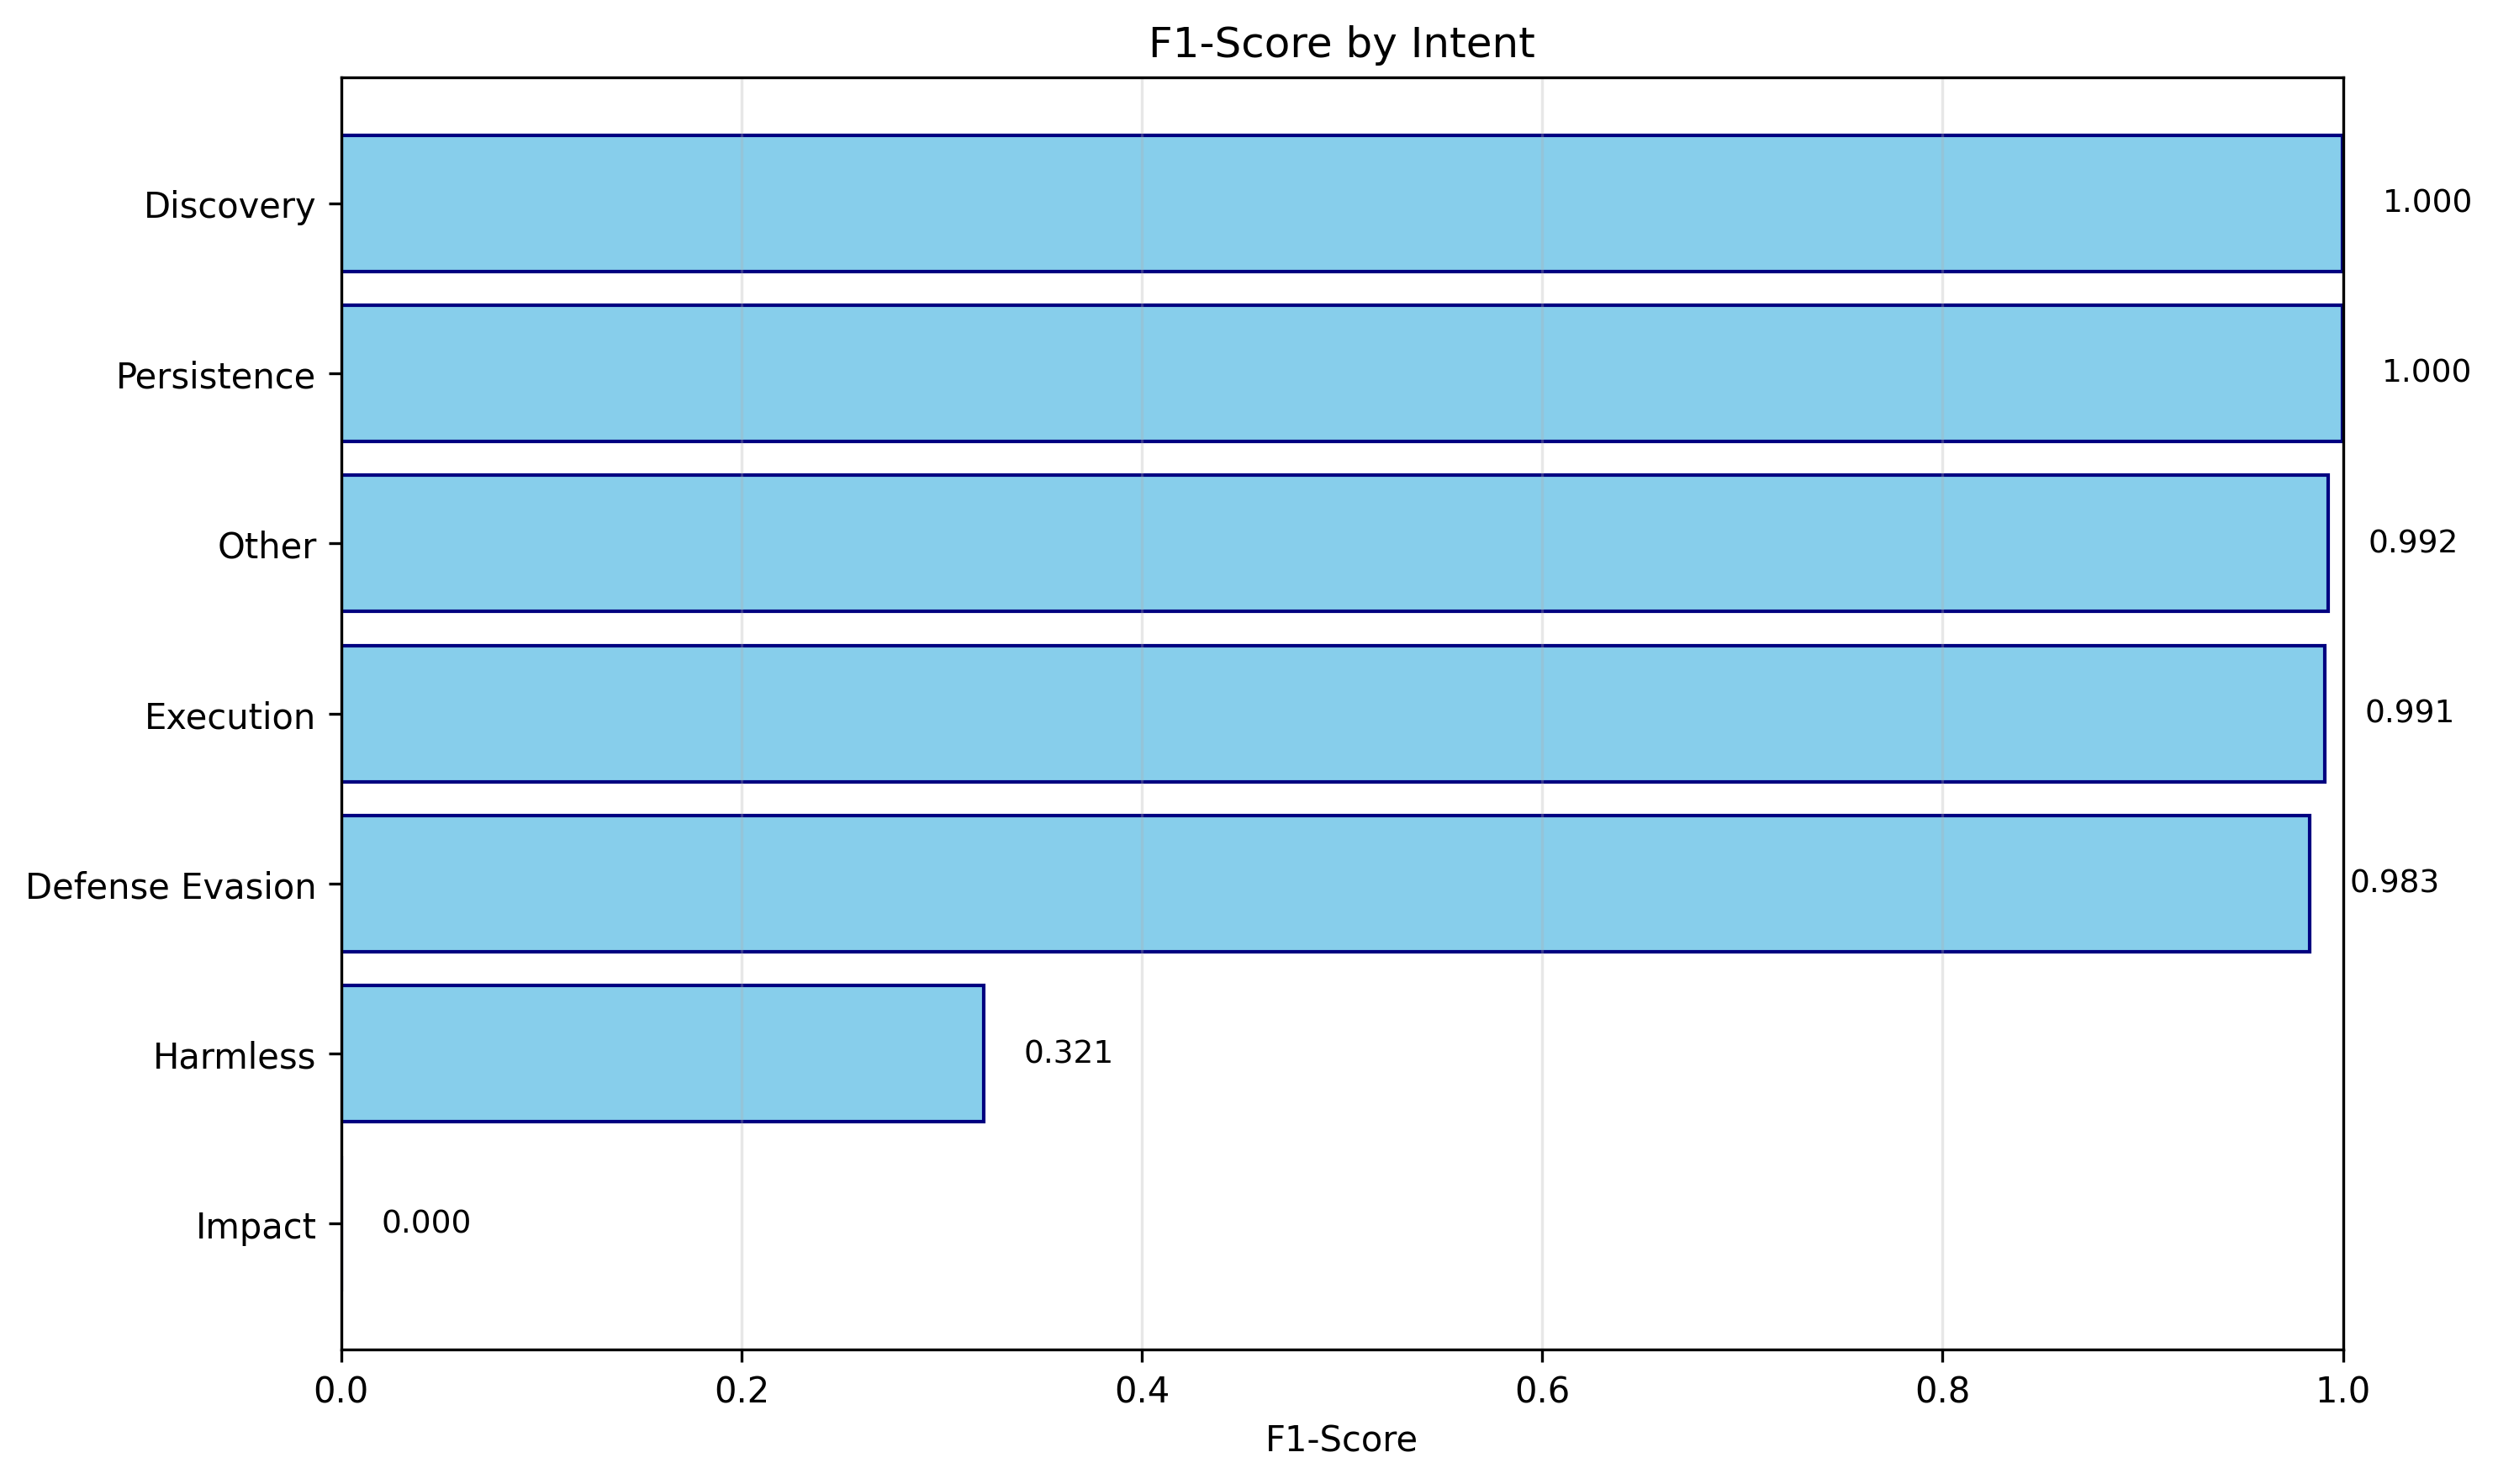
\includegraphics[width=0.7\textwidth]{results/plots/section4/f1_by_intent.png}
\caption{F1-scores by intent showing excellent performance on majority classes but failure on most extreme minority classes.}
\label{fig:f1_by_intent}
\end{figure}


The high micro F1-score (0.9959) reflects the model's strong performance on the abundant majority classes, while the significantly lower macro F1-score (0.7574) reveals the impact of minority class struggles. Despite sophisticated class weighting, the model cannot effectively learn from intents with fewer than 100 samples.

ROC analysis and detailed precision-recall metrics by intent are provided in \hyperref[appendix:D2]{Appendix D.2}, demonstrating strong discrimination capability (AUC > 0.99) for well-represented classes while confirming the statistical impossibility of learning meaningful patterns from 2 training examples.

\subsection{Comparison with Traditional ML Approaches}

Table~\ref{tab:model_comparison} compares BERT with tuned Logistic Regression on the test set:

\begin{table}[htbp]
\centering
\caption{BERT vs tuned Logistic Regression}
\label{tab:model_comparison}
\begin{tabular}{@{}lccc@{}}
\toprule
\textbf{Metric} & \textbf{LR (tuned)} & \textbf{BERT} & \textbf{Improvement} \\
\midrule
Accuracy & 0.9843 & 0.9816 & -0.27\% \\
F1 (Micro) & 0.9964 & 0.9959 & -0.05\% \\
F1 (Macro) & 0.8463 & 0.7574 & -10.50\% \\
Hamming Loss & 0.0157 & 0.0028 & -82.17\% \\
\midrule
\multicolumn{4}{l}{\textit{Per-Intent F1-Scores:}} \\
Discovery & 1.000 & 0.9999 & -0.01\% \\
Persistence & 1.000 & 0.9995 & -0.05\% \\
Execution & 0.990 & 0.9909 & +0.09\% \\
Defense Evasion & 0.980 & 0.9835 & +0.36\% \\
Other & 0.990 & 0.9925 & +0.25\% \\
Harmless & 0.290 & 0.3355 & +15.69\% \\
Impact & 0.670 & 0.0000 & -100.00\% \\
\bottomrule
\end{tabular}
\end{table}


Despite BERT's architectural sophistication, Logistic Regression demonstrates superior overall performance, particularly on macro F1-score (0.8463 vs 0.7574), indicating better minority class handling. The key advantage of LR lies in its effective class weight optimization, achieving 0.67 F1 on Impact (only 2 test samples) while BERT completely fails (0.00). Both models achieve near-identical performance on majority classes, with micro F1-scores above 0.995.

BERT's primary advantage appears in Hamming Loss (0.0028 vs 0.0157), suggesting fewer per-label errors in the multi-label setting. However, this marginal benefit does not compensate for the 10.5\% degradation in macro F1-score and significant computational overhead. For this extremely imbalanced dataset, traditional ML with proper class weighting proves more effective than transfer learning from pre-trained language models.

\subsection{Discussion and Model Selection}


\textbf{Why Traditional ML Wins:} The strong performance of Logistic Regression with TF-IDF features (macro F1: 0.8463) demonstrates that SSH attack patterns are effectively captured by term frequency representations. Discriminative commands such as "wget", "chmod", and "crontab" combined with L2 regularization and class weighting provide excellent classification performance. The probabilistic framework of logistic regression handles extreme class imbalance (e.g., Impact with 2 samples) more effectively than BERT's neural architecture.

\textbf{Computational Trade-offs:} Training time differs dramatically: BERT requires 5-6 hours on GPU compared to LR's 2 minutes on CPU. Similarly, inference latency shows BERT at 32ms per session versus LR at <1ms. Given LR's superior macro F1-score, computational efficiency, and better minority class handling, it represents the optimal choice for production deployment.

\textbf{When BERT Might Excel:} Future datasets with more complex sequential dependencies, natural language descriptions of attacks, or novel attack patterns not well-represented by individual command frequencies might favor BERT's contextual understanding. For this command-focused dataset with clear discriminative features, however, traditional ML proves superior.

% ============================================
% SECTION 6: CONCLUSIONS AND FUTURE WORK
% ============================================
\section{Conclusions and Future Work}

\subsection{Summary of Findings}

This research presented a comprehensive machine learning approach to analyzing SSH shell attack sessions using the MITRE ATT\&CK framework for multi-label intent classification.

\paragraph{Supervised Learning Classification} demonstrated that traditional ML approaches excel on this task:
\begin{itemize}
    \item Tuned Logistic Regression achieved best overall performance: 98.43\% accuracy, 0.8463 macro F1-score
    \item TF-IDF feature representation effectively captured discriminative attack patterns
    \item Outstanding performance on common intents (Discovery, Persistence, Execution) with F1 scores >0.99
    \item Persistent challenges with extreme minority classes (Impact: 2 samples, Harmless: 458 samples)
\end{itemize}

\paragraph{Unsupervised Learning Clustering} uncovered fine-grained attack patterns:
\begin{itemize}
    \item Optimal clustering at k=10 with high algorithm agreement (ARI=0.82, NMI=0.84)
    \item Weighted average cluster purity of 97.75\% indicating highly homogeneous groupings
    \item Six distinct attack categories aligned with MITRE ATT\&CK intents
    \item Revealed co-occurrence patterns between Discovery and Persistence intents
\end{itemize}

\paragraph{BERT Language Model} showed strong but not superior performance:
\begin{itemize}
    \item Competitive overall metrics: 98.16\% accuracy, 0.7574 macro F1-score
    \item Near-perfect performance on majority classes (Discovery: 0.9999, Persistence: 0.9995)
    \item Complete failure on Impact class (F1=0.00) despite class weighting
    \item Superior Hamming Loss (0.0028 vs 0.0157) indicating fewer per-label errors
    \item Computational overhead (5-6 hours training, 32ms inference) limits practical deployment
\end{itemize}

\subsection{Best Performing Approach}

The \textbf{tuned Logistic Regression model} emerged as the optimal approach for production deployment:

\begin{itemize}
    \item \textbf{Superior Macro F1}: 0.8463 vs BERT's 0.7574, demonstrating better minority class handling
    \item \textbf{Computational Efficiency}: <1ms inference vs BERT's 32ms, 2-minute training vs 5-6 hours
    \item \textbf{Better Generalization}: Minimal overfitting with consistent train/test performance
    \item \textbf{Interpretability}: Feature coefficients provide actionable insights for security analysts
    \item \textbf{Deployment Simplicity}: Small model size (<5MB) suitable for edge deployment
\end{itemize}

This demonstrates that for command-based attack logs with clear discriminative features, carefully tuned traditional ML with proper class weighting outperforms sophisticated neural architectures.

\subsection{Limitations}

\paragraph{Class Imbalance} remains the dominant challenge:
\begin{itemize}
    \item Extreme imbalance ratios (Impact: 2 samples, Discovery: 46,433 samples = 23,000:1 ratio)
    \item Both traditional ML and BERT struggle with <100 training examples per class
    \item Class weighting provides partial mitigation but cannot overcome statistical insufficiency
\end{itemize}

\paragraph{Dataset Characteristics}:
\begin{itemize}
    \item Honeypot data may not represent all real-world attack scenarios
    \item Temporal coverage (June 2019-February 2020) might miss evolving attack patterns
    \item Multi-label complexity (average 2-3 intents per session) increases classification difficulty
\end{itemize}

\paragraph{Model Selection Trade-offs}:
\begin{itemize}
    \item BERT's contextual understanding underutilized for command-based logs
    \item Computational requirements limit BERT's real-time deployment feasibility
    \item Intent dependencies not explicitly modeled in current approaches
\end{itemize}

\subsection{Future Research Directions}

\paragraph{Addressing Class Imbalance}:
\begin{itemize}
    \item \textbf{Synthetic Data Generation}: Create realistic rare attack samples using rule-based systems and command templates
    \item \textbf{Few-Shot Learning}: Leverage meta-learning techniques to improve performance with limited examples
    \item \textbf{Active Learning}: Prioritize labeling of uncertain or rare attack patterns from new honeypot data
\end{itemize}

\paragraph{Advanced Modeling}:
\begin{itemize}
    \item \textbf{Label Dependency Modeling}: Implement classifier chains to explicitly model intent co-occurrence
    \item \textbf{Ensemble Methods}: Combine BERT's contextual understanding with LR's efficiency
    \item \textbf{Domain-Specific Pre-training}: Train language models specifically on security logs and attack datasets
\end{itemize}

\paragraph{Deployment and Explainability}:
\begin{itemize}
    \item Real-time streaming classification pipeline integrated with SIEM systems
    \item Attention visualization and SHAP analysis for interpretable predictions
    \item Temporal pattern analysis to detect evolving attack campaigns
    \item Automated threat intelligence generation from classified sessions
\end{itemize}

\subsection{Practical Impact}

This research provides actionable capabilities for cybersecurity operations:

\begin{enumerate}
    \item \textbf{Automated Threat Analysis}: Classification of thousands of attack sessions with 98\%+ accuracy reduces manual analyst workload
    
    \item \textbf{Attack Pattern Discovery}: Clustering reveals six distinct attack categories, enabling early detection of emerging threats
    
    \item \textbf{Incident Prioritization}: Intent classification allows focus on high-impact attacks (Persistence, Impact) over reconnaissance
    
    \item \textbf{Threat Intelligence Sharing}: Fine-grained categorization supports IOC generation aligned with MITRE ATT\&CK framework
\end{enumerate}

\subsection{Concluding Remarks}

This research demonstrates that traditional machine learning with carefully engineered TF-IDF features remains highly competitive with modern deep learning approaches for SSH attack classification. The tuned Logistic Regression model achieves 98.43\% accuracy and 0.8463 macro F1-score, outperforming BERT (98.16\% accuracy, 0.7574 macro F1-score) while providing superior computational efficiency and interpretability.

The key insight is that \textbf{class imbalance}, not model architecture, \textbf{ is the limiting factor} for this task. Both traditional ML and BERT fail on extreme minority classes with fewer than 100 samples. Addressing this through synthetic data generation, few-shot learning, or active labeling represents the most promising direction for improvement.

Unsupervised clustering with 97.75\% purity successfully identifies six distinct attack categories, demonstrating strong alignment with MITRE ATT\&CK intents. This combined supervised-unsupervised approach provides a comprehensive framework for automated threat analysis in security operations.

As cyber threats evolve, machine learning-powered log analysis will become increasingly critical. This research provides a practical foundation for deploying accurate, efficient, and interpretable attack classification systems in real-world security contexts.

% ============================================
% REFERENCES
% ============================================
\begin{thebibliography}{8}

\bibitem{mitre_attack}
MITRE ATT\&CK Framework.
\newblock \url{https://attack.mitre.org/}
\newblock Accessed: 2025-01-15.

\bibitem{devlin2018bert}
Jacob Devlin, Ming-Wei Chang, Kenton Lee, and Kristina Toutanova.
\newblock BERT: Pre-training of Deep Bidirectional Transformers for Language Understanding.
\newblock In \textit{Proceedings of NAACL-HLT 2019}, pages 4171--4186, 2019.

\bibitem{tsoumakas2007multi}
Grigorios Tsoumakas and Ioannis Katakis.
\newblock Multi-Label Classification: An Overview.
\newblock \textit{International Journal of Data Warehousing and Mining}, 3(3):1--13, 2007.

\bibitem{rousseeuw1987silhouettes}
Peter J. Rousseeuw.
\newblock Silhouettes: A Graphical Aid to the Interpretation and Validation of Cluster Analysis.
\newblock \textit{Journal of Computational and Applied Mathematics}, 20:53--65, 1987.

\bibitem{maaten2008visualizing}
Laurens van der Maaten and Geoffrey Hinton.
\newblock Visualizing Data using t-SNE.
\newblock \textit{Journal of Machine Learning Research}, 9:2579--2605, 2008.

\bibitem{honeypot_ssh}
Niels Provos.
\newblock A Virtual Honeypot Framework.
\newblock In \textit{Proceedings of USENIX Security Symposium}, volume 173, pages 1--14, 2004.

\bibitem{intrusion_detection_ml}
Robin Sommer and Vern Paxson.
\newblock Outside the Closed World: On Using Machine Learning for Network Intrusion Detection.
\newblock In \textit{IEEE Symposium on Security and Privacy}, pages 305--316, 2010.

\bibitem{log_analysis_ml}
Min Du et al.
\newblock DeepLog: Anomaly Detection and Diagnosis from System Logs through Deep Learning.
\newblock In \textit{Proceedings of ACM CCS 2017}, pages 1285--1298, 2017.

\end{thebibliography}

% ============================================================
% APPENDICES
% ============================================================
\appendix
\clearpage
%% ============================================================
%% APPENDIX A: EXTENDED DATA EXPLORATION ANALYSIS
%% ============================================================
\section{Extended Data Exploration Analysis}
\addcontentsline{toc}{section}{Appendix A: Supplementary Data Exploration Results}

\subsection{Session Characteristics}
\label{appendix:A1}
\addcontentsline{toc}{subsection}{A.1 Session Characteristics}

\begin{figure}[H]
  \centering
  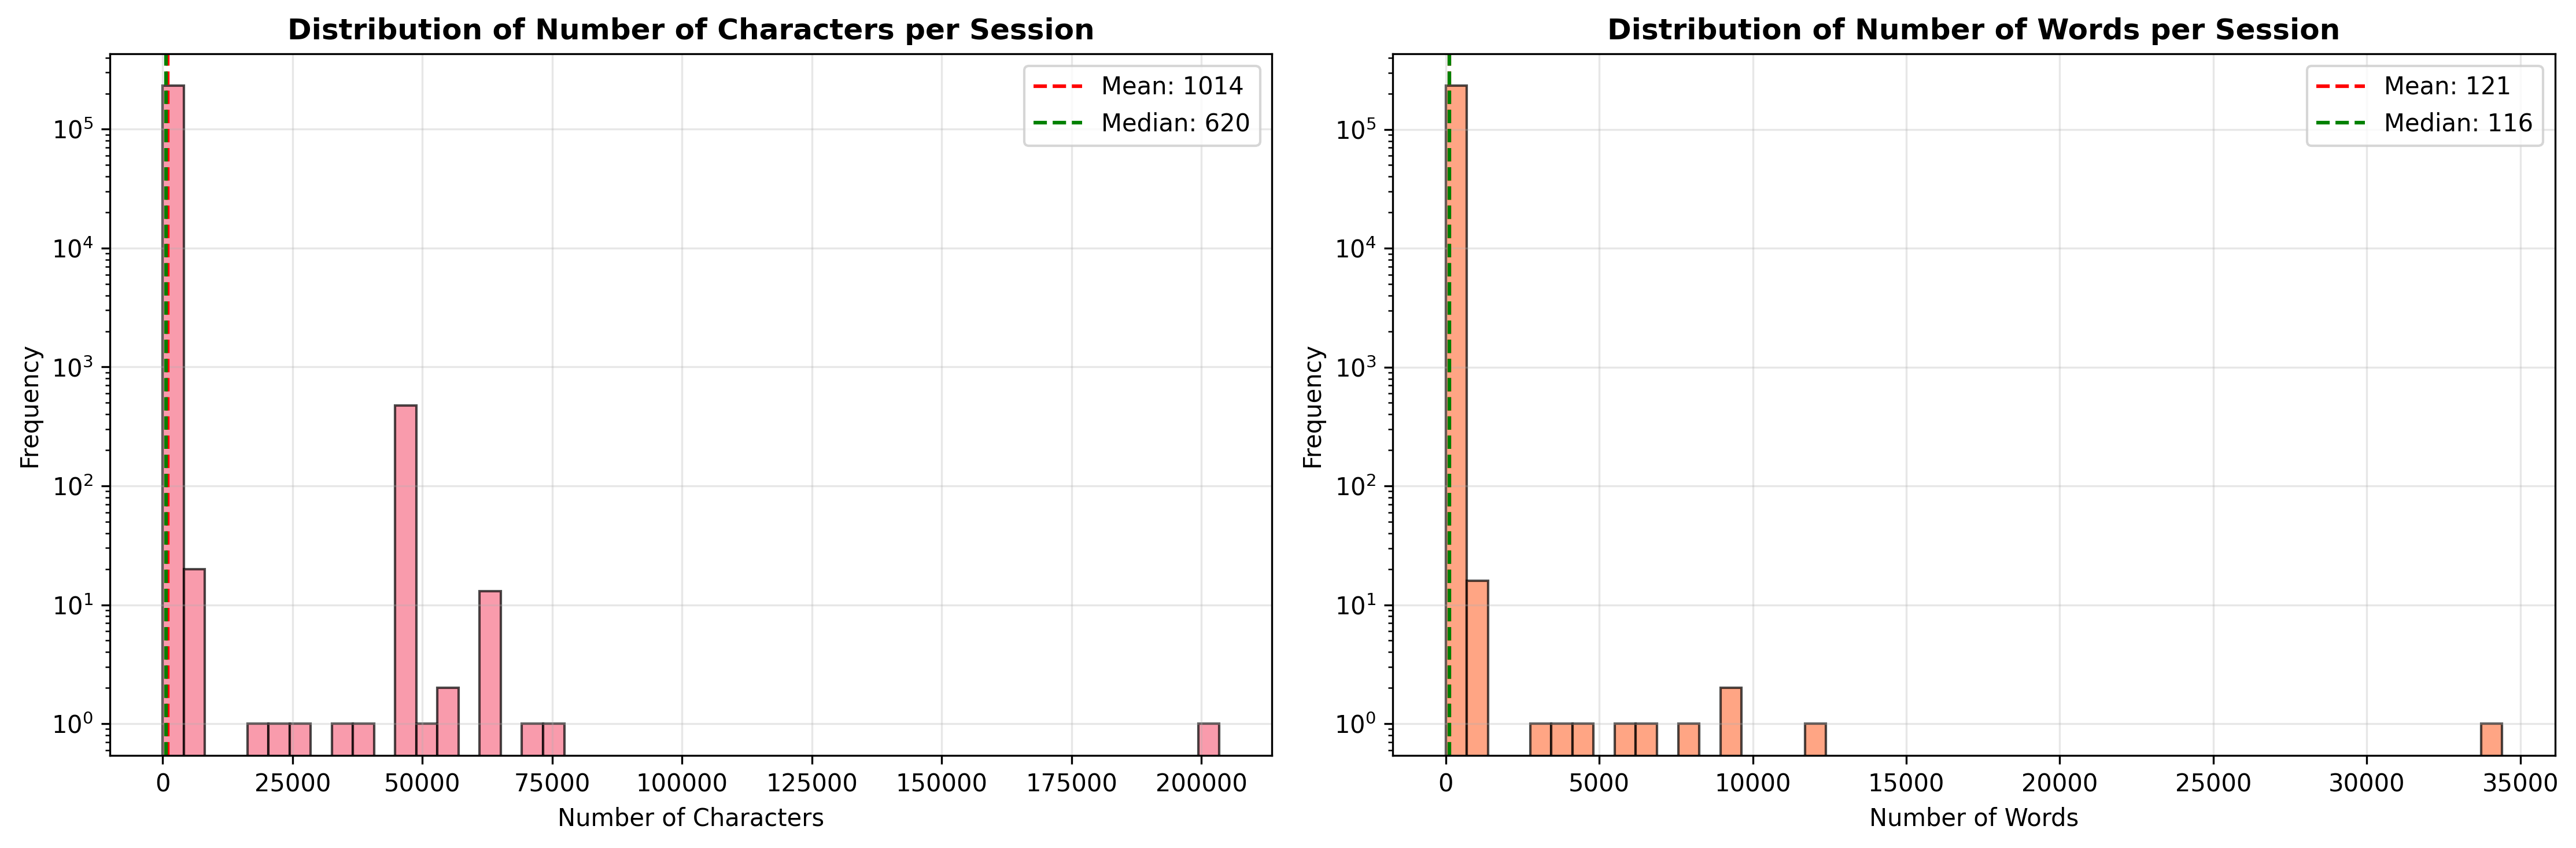
\includegraphics[width=1.0\textwidth]{results/plots/section1/char_word_distributions.png}
  \caption{Distribution of character counts (left) and word counts (right) per session. Character distribution: mean 1,014, median 620. Word distribution: mean 121, median 116. Long tails indicate complex multi-stage attacks with extensive command sequences.}
  \label{fig:char_word_dist_appendix}
\end{figure}

\subsection{Vocabulary Analysis}
\label{appendix:A2}
\addcontentsline{toc}{subsection}{A.2 Vocabulary Analysis}

\begin{figure}[H]
  \centering
  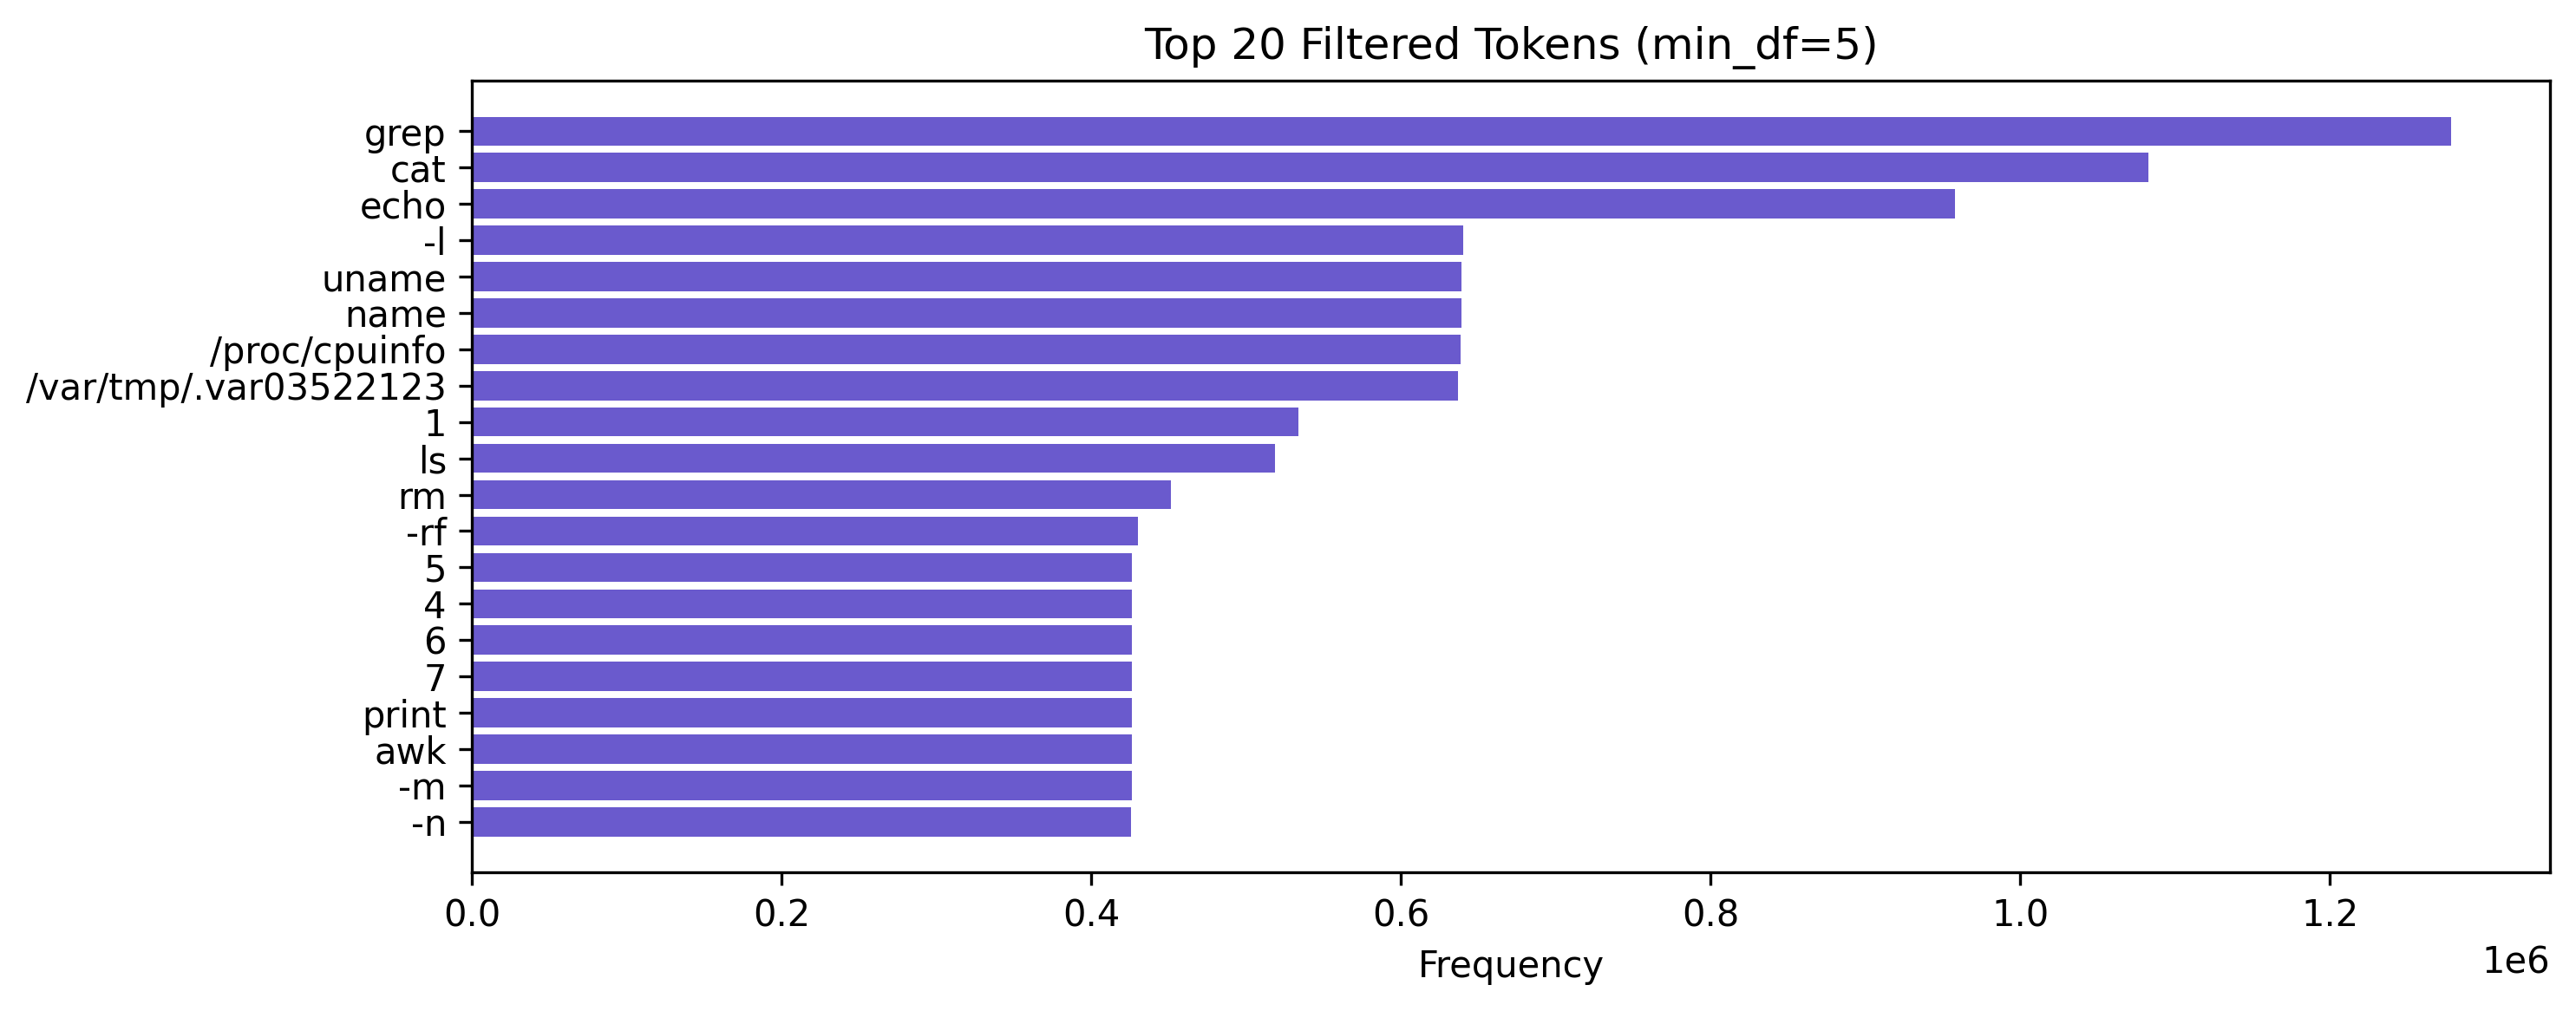
\includegraphics[width=1.0\textwidth]{results/plots/section1/top_tokens.png}
  \caption{Top 20 tokens: Recon-focused (grep ~1.2e6 occurrences), indicating system probing.}
  \label{fig:top_tokens_appendix}
\end{figure}

\subsection{Temporal Intent Evolution}
\label{appendix:A3}
\addcontentsline{toc}{subsection}{A.3 Temporal Intent Evolution}

\begin{figure}[H]
  \centering
  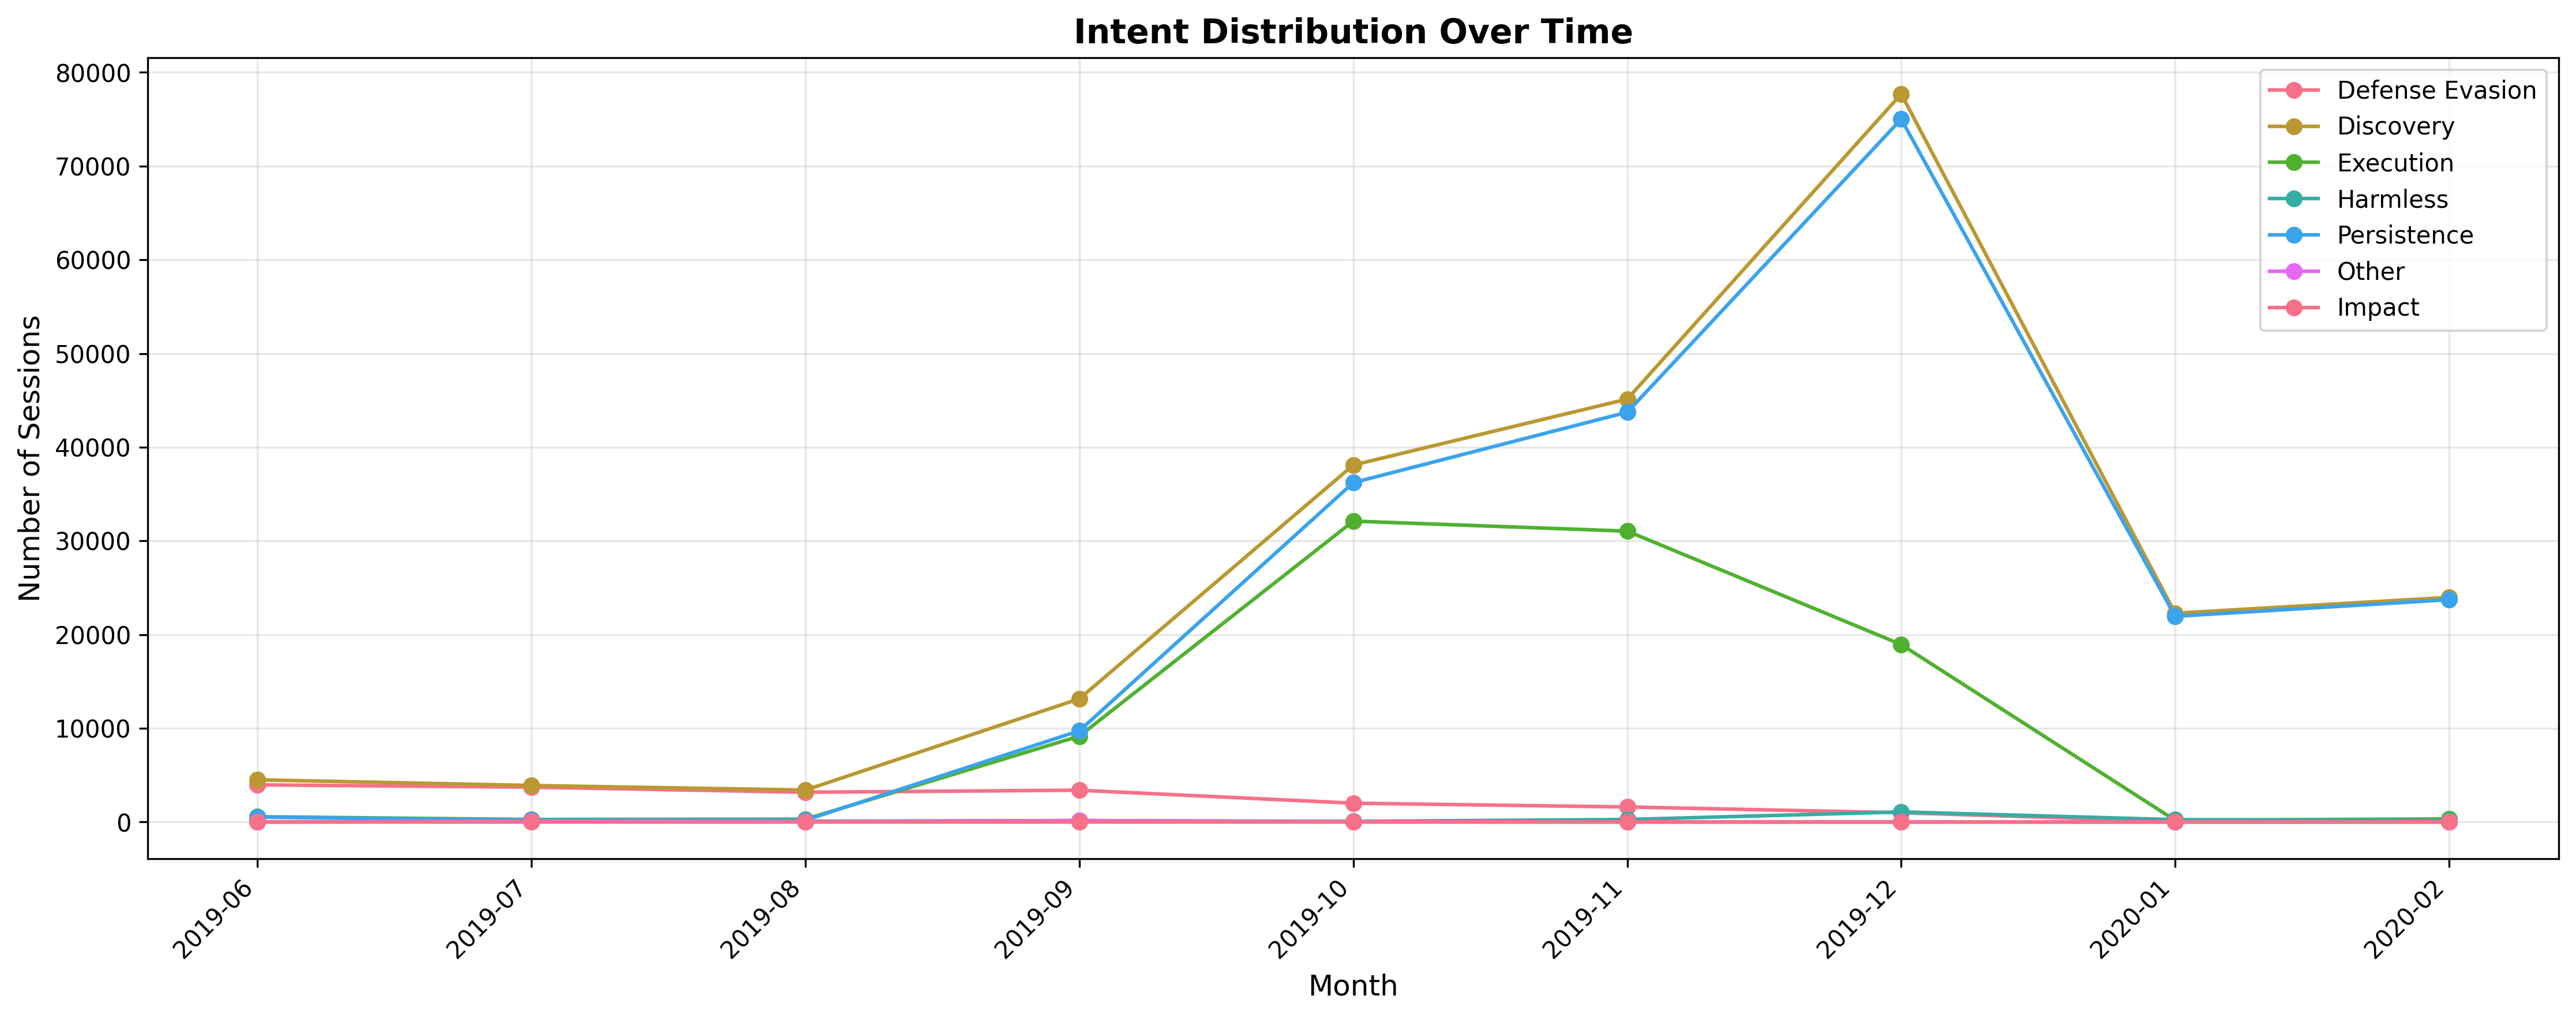
\includegraphics[width=1.0\textwidth]{results/plots/section1/intent_over_time.png}
  \caption{Intent trends: Discovery/Persistence steady; Execution/Impact peak December 2019.}
  \label{fig:intent_time_appendix}
\end{figure}

%% ============================================================
%% APPENDIX B: EXTENDED SUPERVISED LEARNING RESULTS
%% ============================================================
\section{Extended Supervised Learning Results}
\addcontentsline{toc}{section}{Appendix B: Extended Supervised Learning Results}

\subsection{Feature Importance Analysis}
\label{appendix:B1}
\addcontentsline{toc}{subsection}{B.1 Feature Importance Analysis}

\begin{figure}[H]
  \centering
  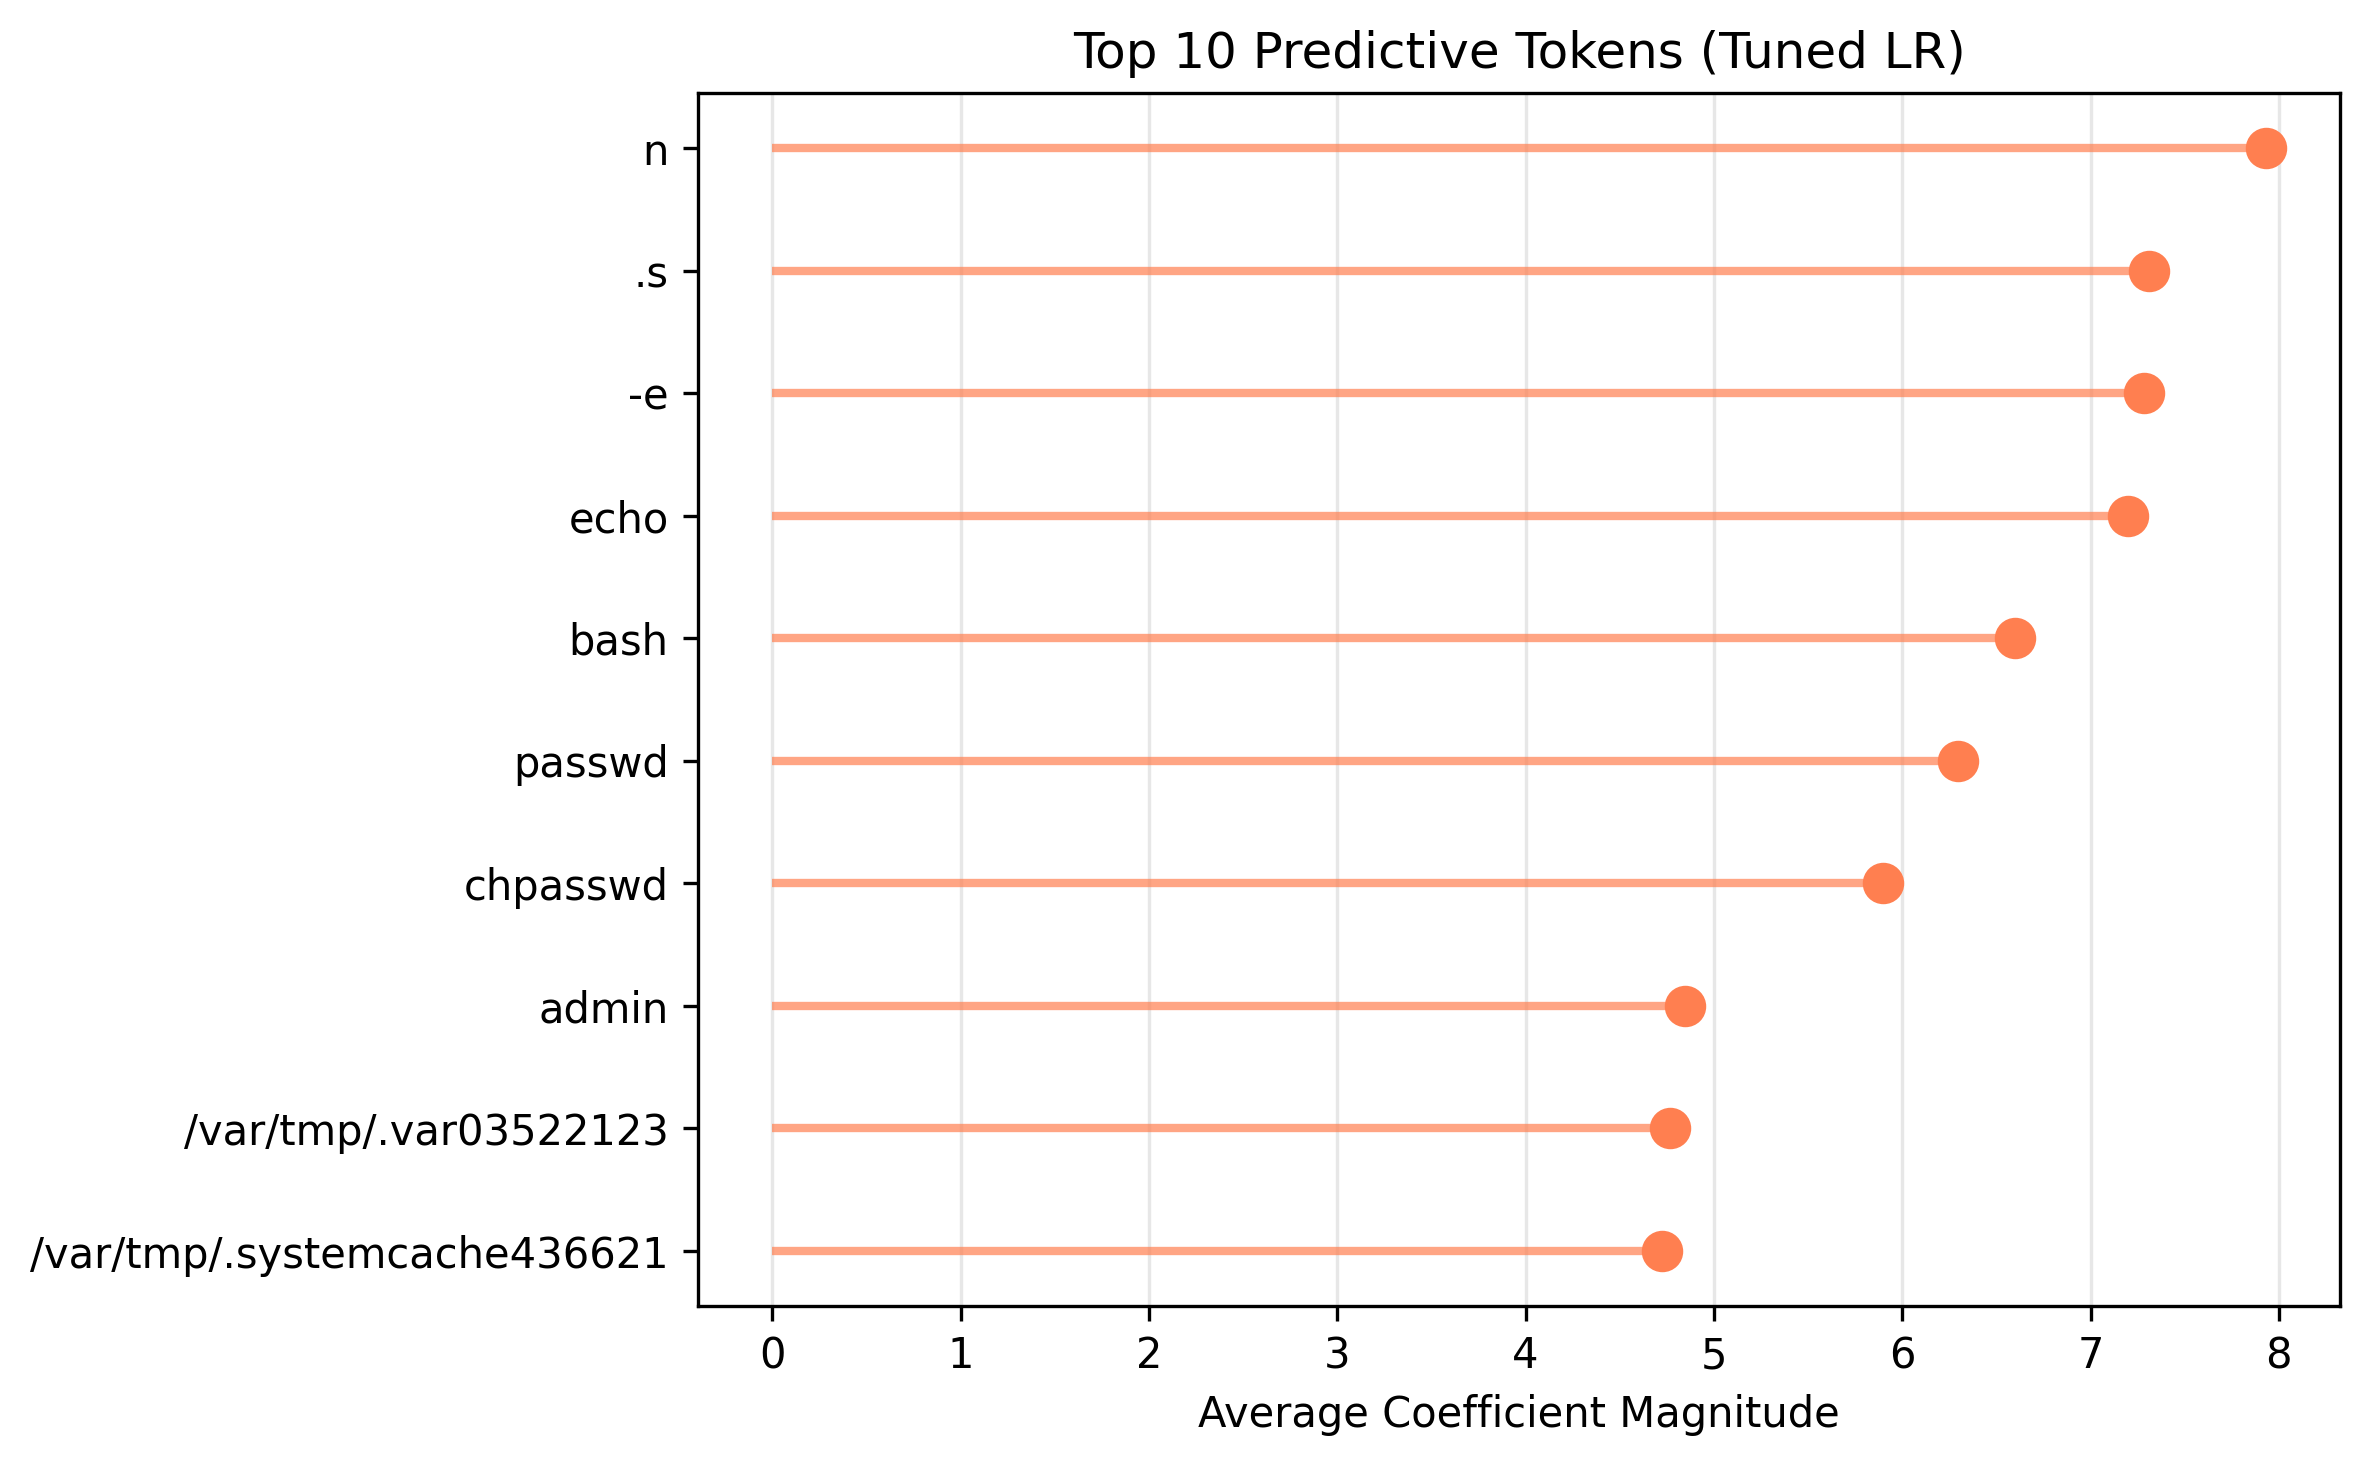
\includegraphics[width=0.8\textwidth]{results/plots/section2/top_predictive_tokens.png}
  \caption{Top predictive tokens (tuned LR): Encoded paths and admin/passwd dominate, signaling persistence/evasion tactics amid command noise.}
  \label{fig:top_predictive_appendix}
\end{figure}

\clearpage
%% ============================================================
%% APPENDIX C: EXTENDED CLUSTERING ANALYSIS
%% ============================================================
\section{Extended Clustering Analysis}
\addcontentsline{toc}{section}{Appendix C: Extended Clustering Analysis}

This appendix contains supplementary clustering visualizations and validation metrics that complement the main unsupervised learning analysis.

\subsection{Dimensionality Reduction Visualizations}
\label{appendix:C1}
\addcontentsline{toc}{subsection}{C.1 Dimensionality Reduction Visualizations}


\begin{figure}[htbp]
\centering
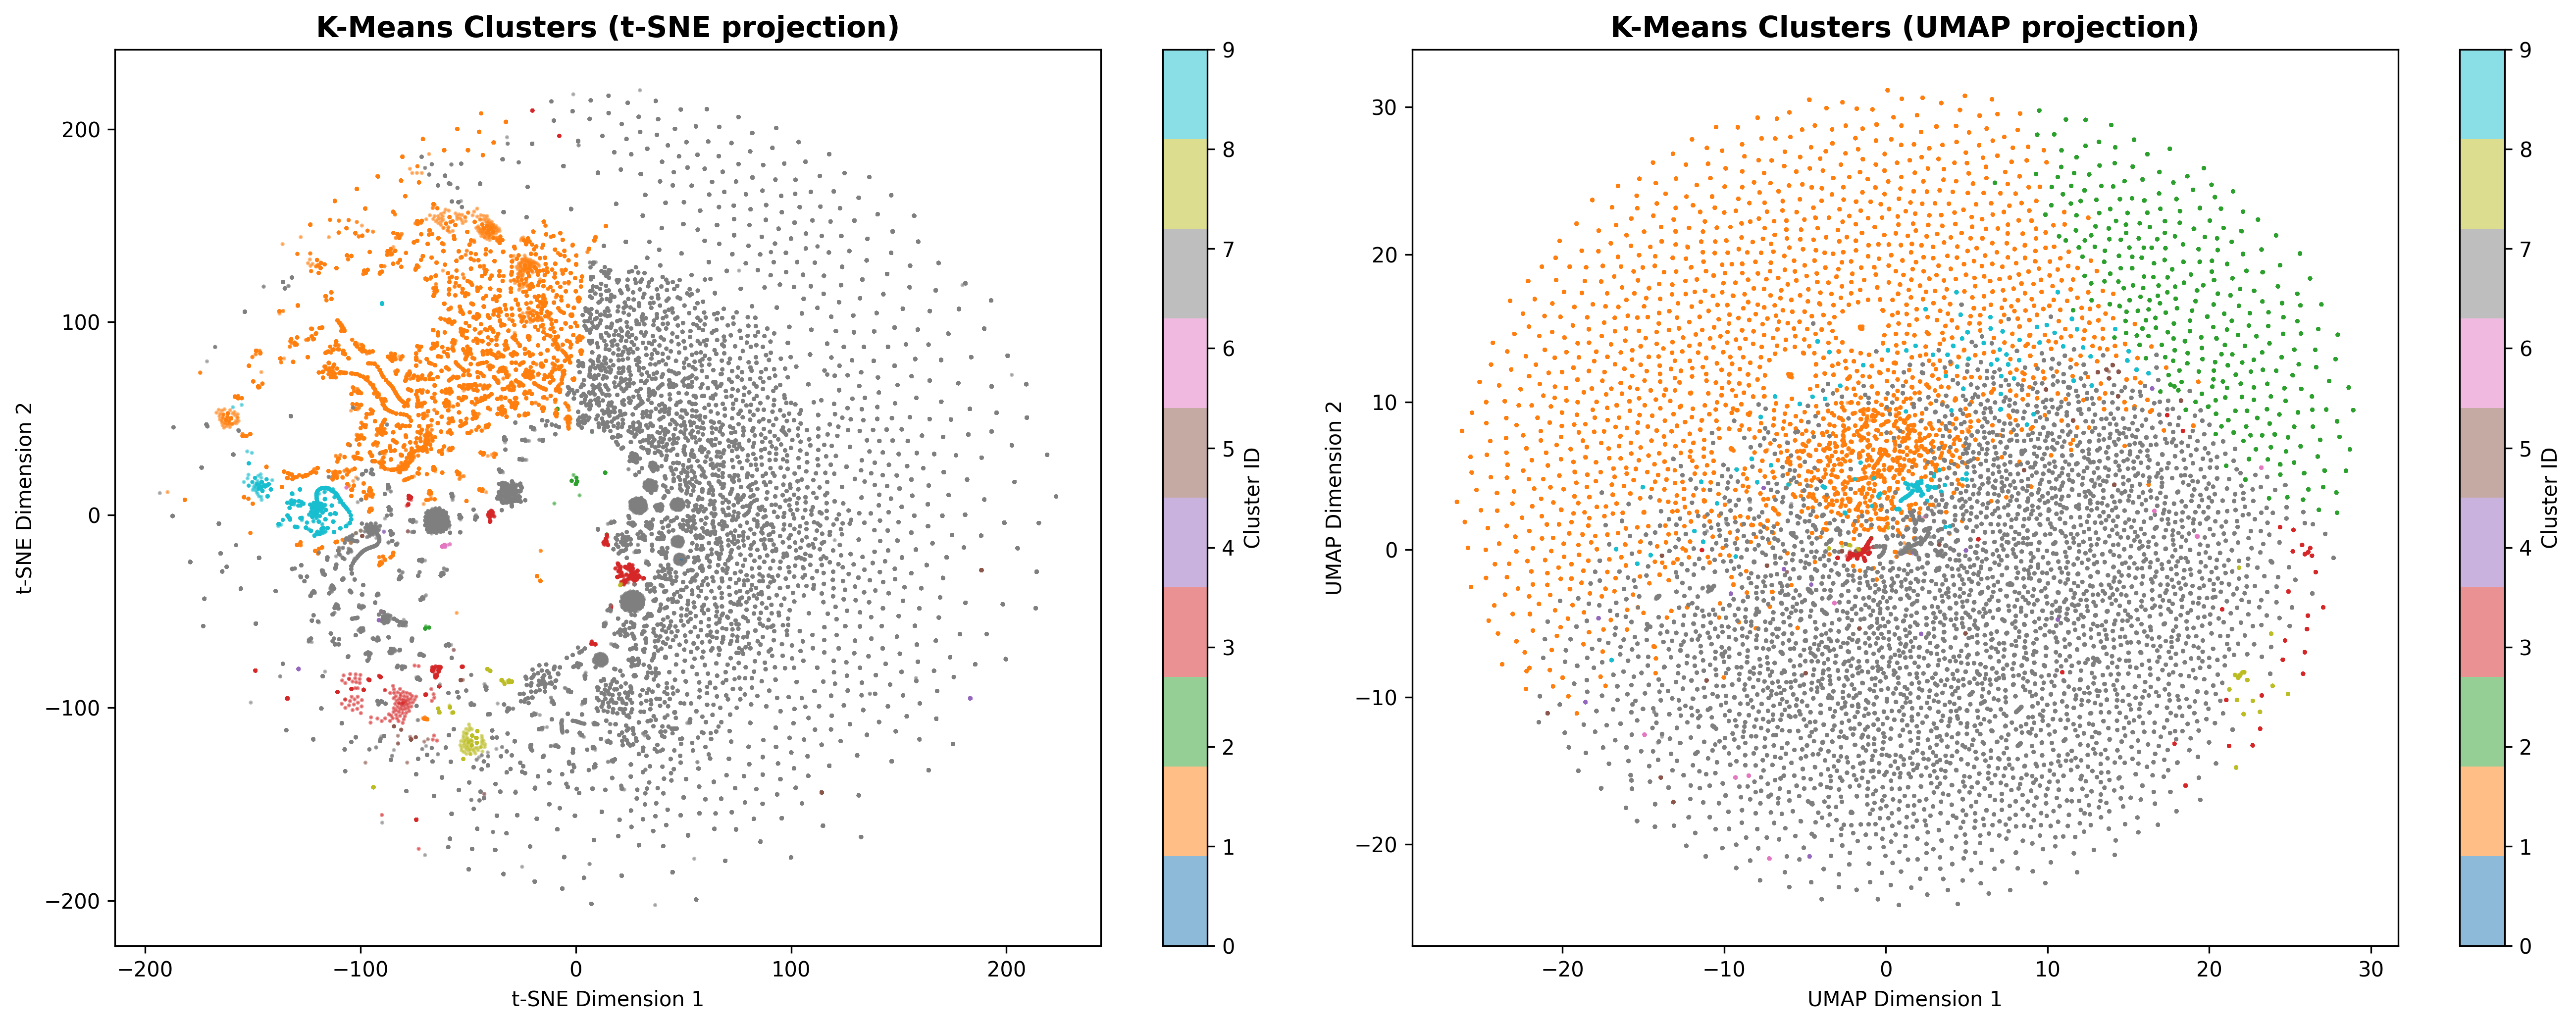
\includegraphics[width=0.9\textwidth]{results/plots/section3/kmeans_clusters_visualization.png}
\caption{K-Means cluster visualization using t-SNE (left) and UMAP (right) dimensionality reduction. Both projections reveal reasonable cluster separation with expected overlap between related attack types. The largest cluster (gray, likely Cluster 1 with 84,047 sessions) dominates the center, while smaller specialized clusters (colored) form distinct periphery regions.}
\label{fig:cluster_visualization_appendix}
\end{figure}

\FloatBarrier
\subsection{Clustering Algorithm Comparison}
\label{appendix:C2}
\addcontentsline{toc}{subsection}{C.2 Clustering Algorithm Comparison}

\begin{figure}[htbp]
\centering
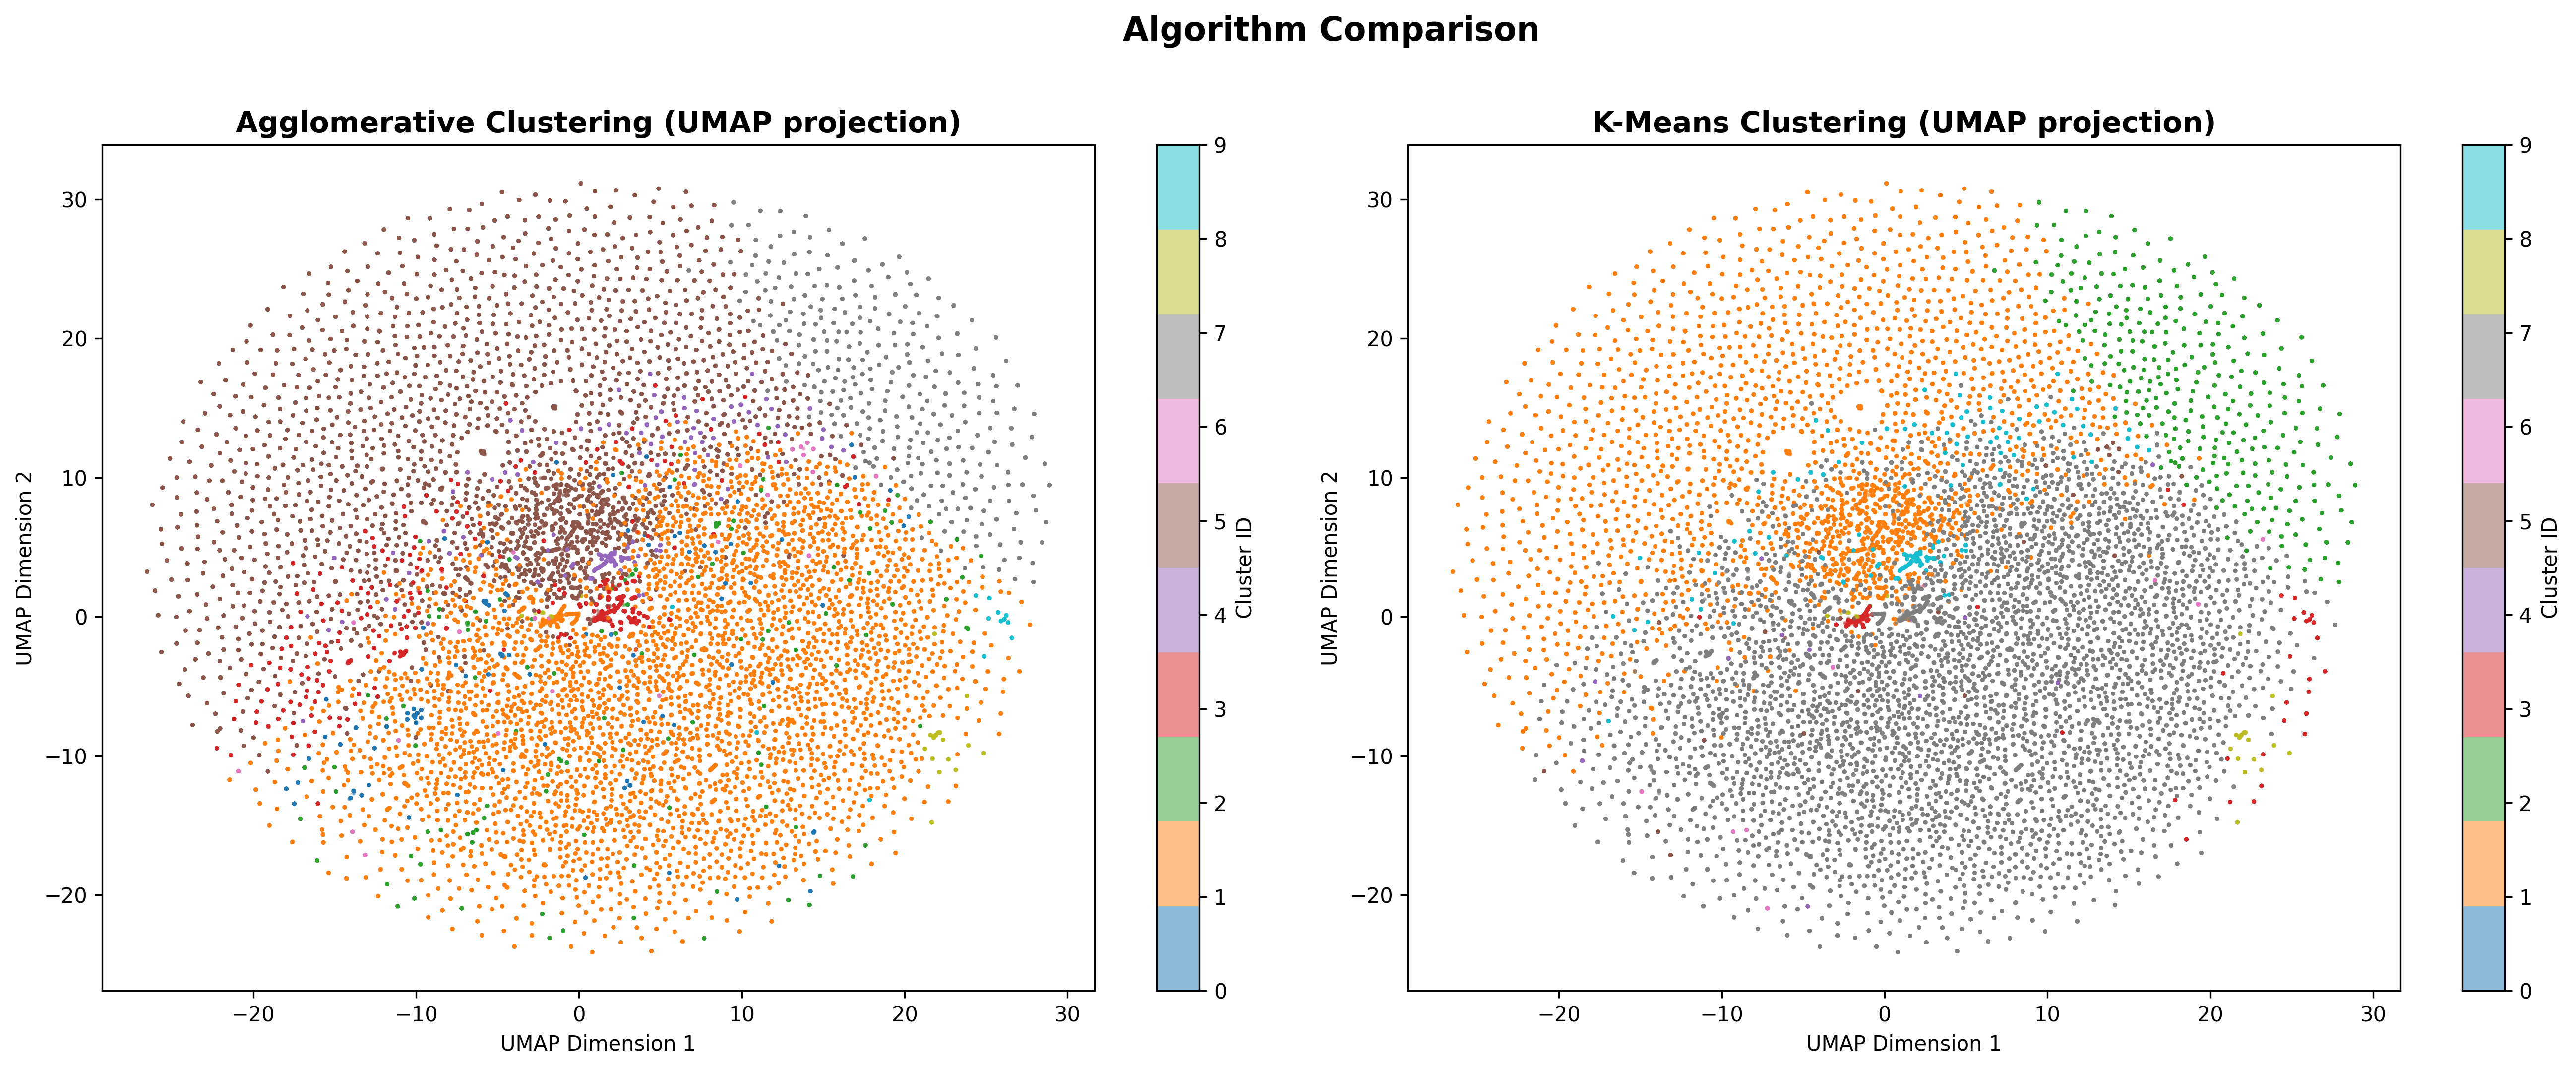
\includegraphics[width=0.9\textwidth]{results/plots/section3/algorithm_comparison.png}
\caption{Algorithm comparison using UMAP projection. Left: Agglomerative Hierarchical clustering with Ward linkage. Right: K-Means clustering. High visual similarity and quantitative agreement (ARI=0.8192, NMI=0.8385) validate consistent pattern discovery across algorithmic approaches.}
\label{fig:algorithm_comparison_appendix}
\end{figure}

\begin{figure}[htbp]
\centering
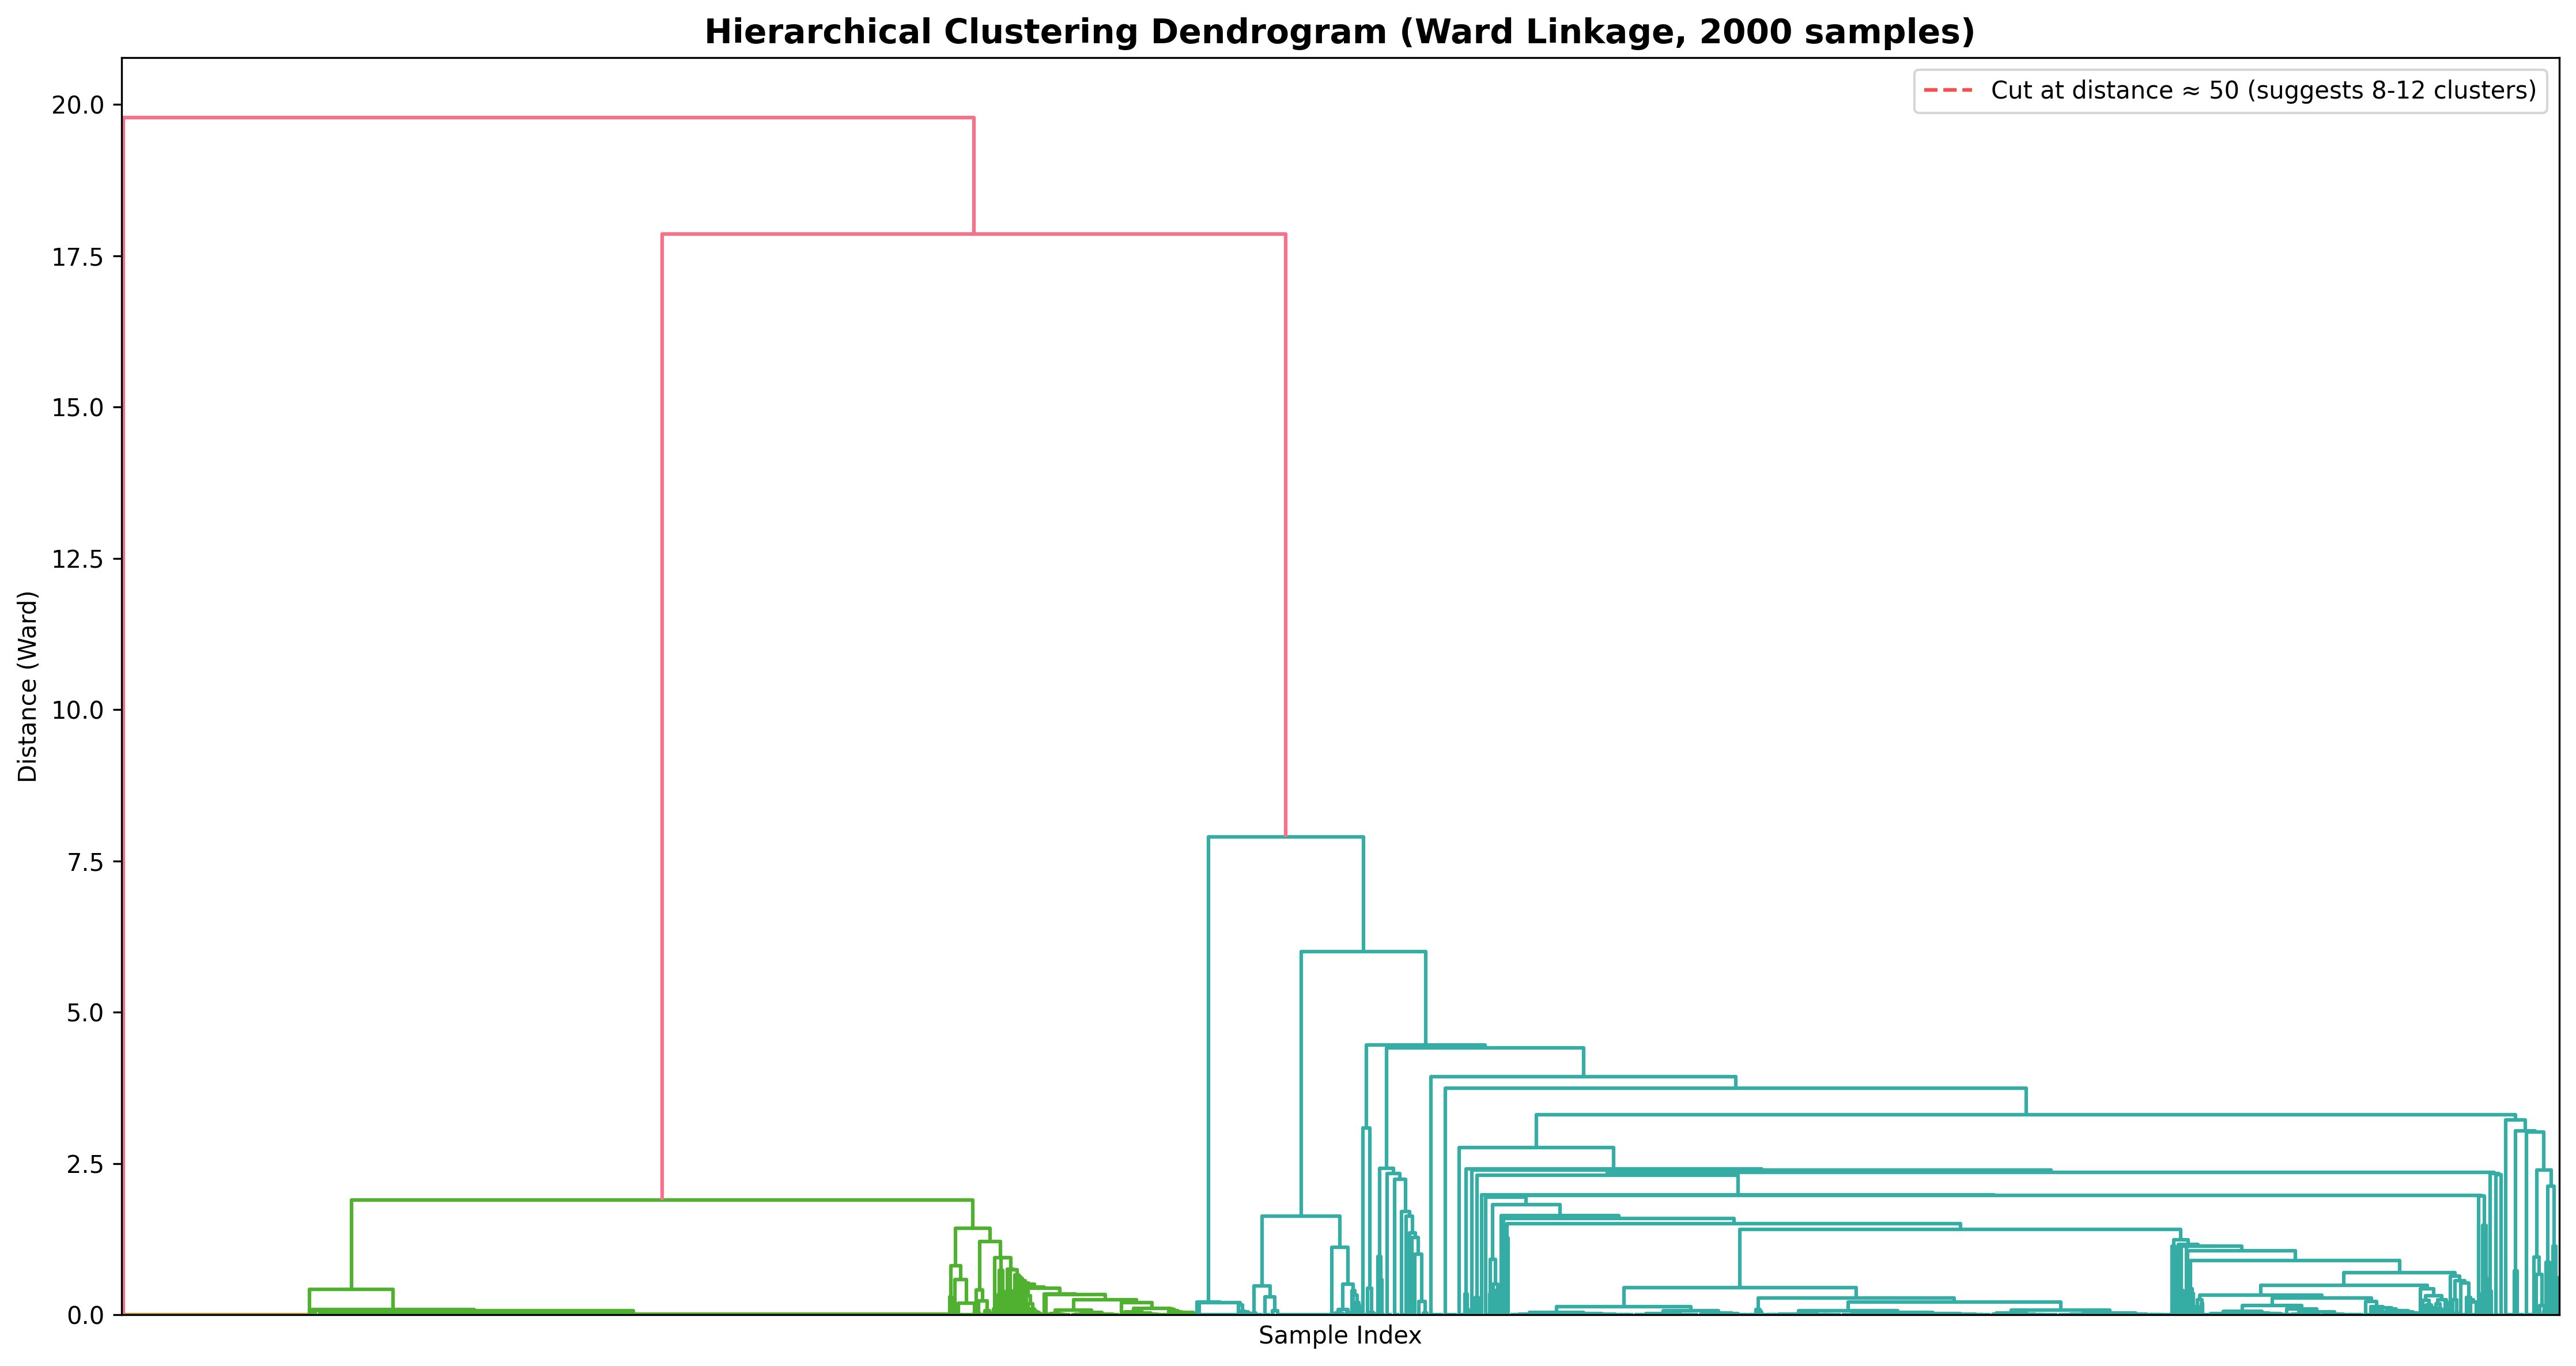
\includegraphics[width=0.85\textwidth]{results/plots/section3/hierarchical_dendrogram.png}
\caption{Hierarchical clustering dendrogram using Ward linkage on 2,000 sample subset. The suggested cut at distance $\approx$ 50 yields 8-12 clusters, consistent with K-Means optimal k=10. Large distance jumps at the top indicate well-separated major cluster groups.}
\label{fig:hierarchical_dendrogram_appendix}
\end{figure}

\FloatBarrier
\subsection{Complete Cluster Profiles}
\label{appendix:C3}
\addcontentsline{toc}{subsection}{C.3 Complete Cluster Profiles}


\begin{figure}[htbp]
\centering
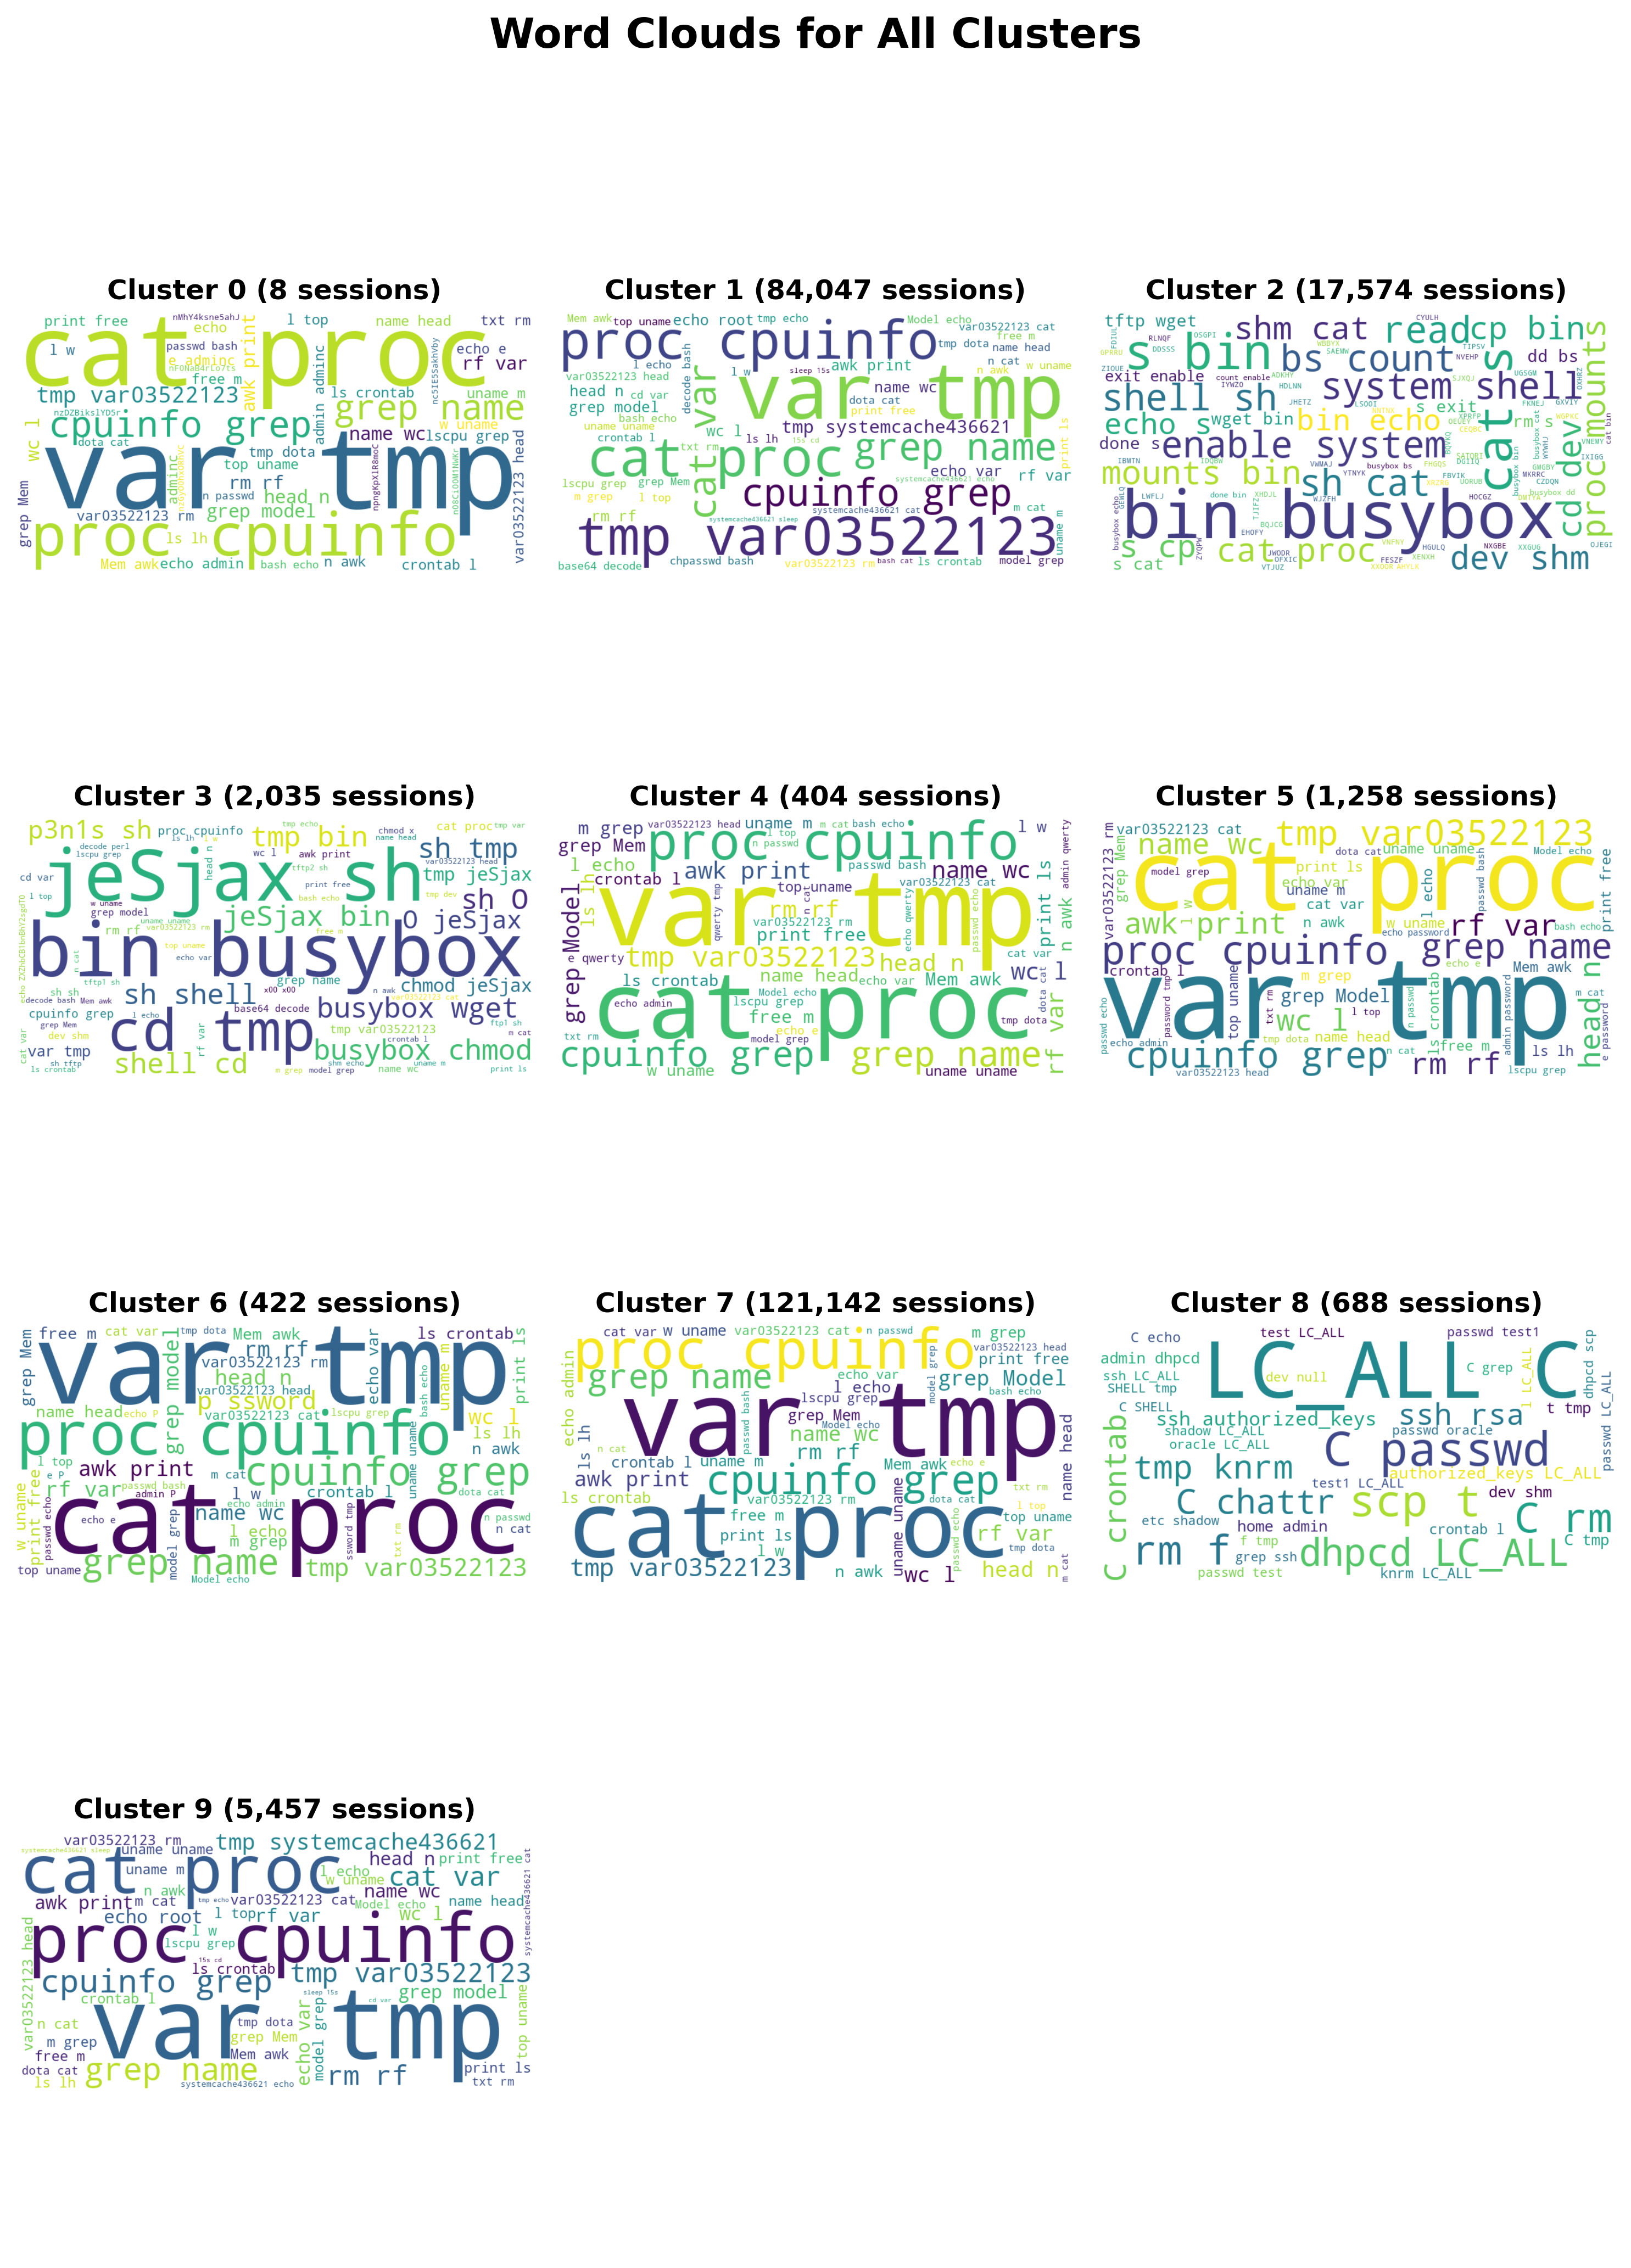
\includegraphics[width=\textwidth]{results/plots/section3/all_cluster_wordclouds.png}
\caption{Complete word cloud visualization for all 10 clusters. Font size indicates term frequency within each cluster. Session counts shown in parentheses.}
\label{fig:all_cluster_wordclouds}
\end{figure}

\begin{table}[htbp]
\centering
\caption{Statistical profiles for all 10 clusters, including dominant intent, purity, and session counts.}
\label{tab:cluster_profiles}
\begin{tabular}{lccc}
\toprule
\textbf{Cluster ID} & \textbf{Dominant Intent} & \textbf{Purity (\%)} & \textbf{Sessions} \\
\midrule
0 & Persistence        & 87.5  & 8        \\
1 & Execution          & 99.4  & 84,047   \\
2 & Defense Evasion    & 99.3  & 17,574   \\
3 & Execution          & 77.1  & 2,035    \\
4 & Persistence        & 97.0  & 404      \\
5 & Persistence        & 98.8  & 1,258    \\
6 & Persistence        & 99.5  & 422      \\
7 & Persistence        & 96.6  & 121,142  \\
8 & Execution          & 97.7  & 688      \\
9 & Execution          & 100.0 & 5,457    \\
\midrule
\multicolumn{2}{l}{\textbf{Weighted Average Purity}} & \textbf{97.75} & \\
\bottomrule
\end{tabular}
\end{table}

\FloatBarrier
\subsection{Intent Composition by Cluster}
\label{appendix:C4}
\addcontentsline{toc}{subsection}{C.4 Intent Composition by Cluster}

\begin{figure}[htbp]
\centering
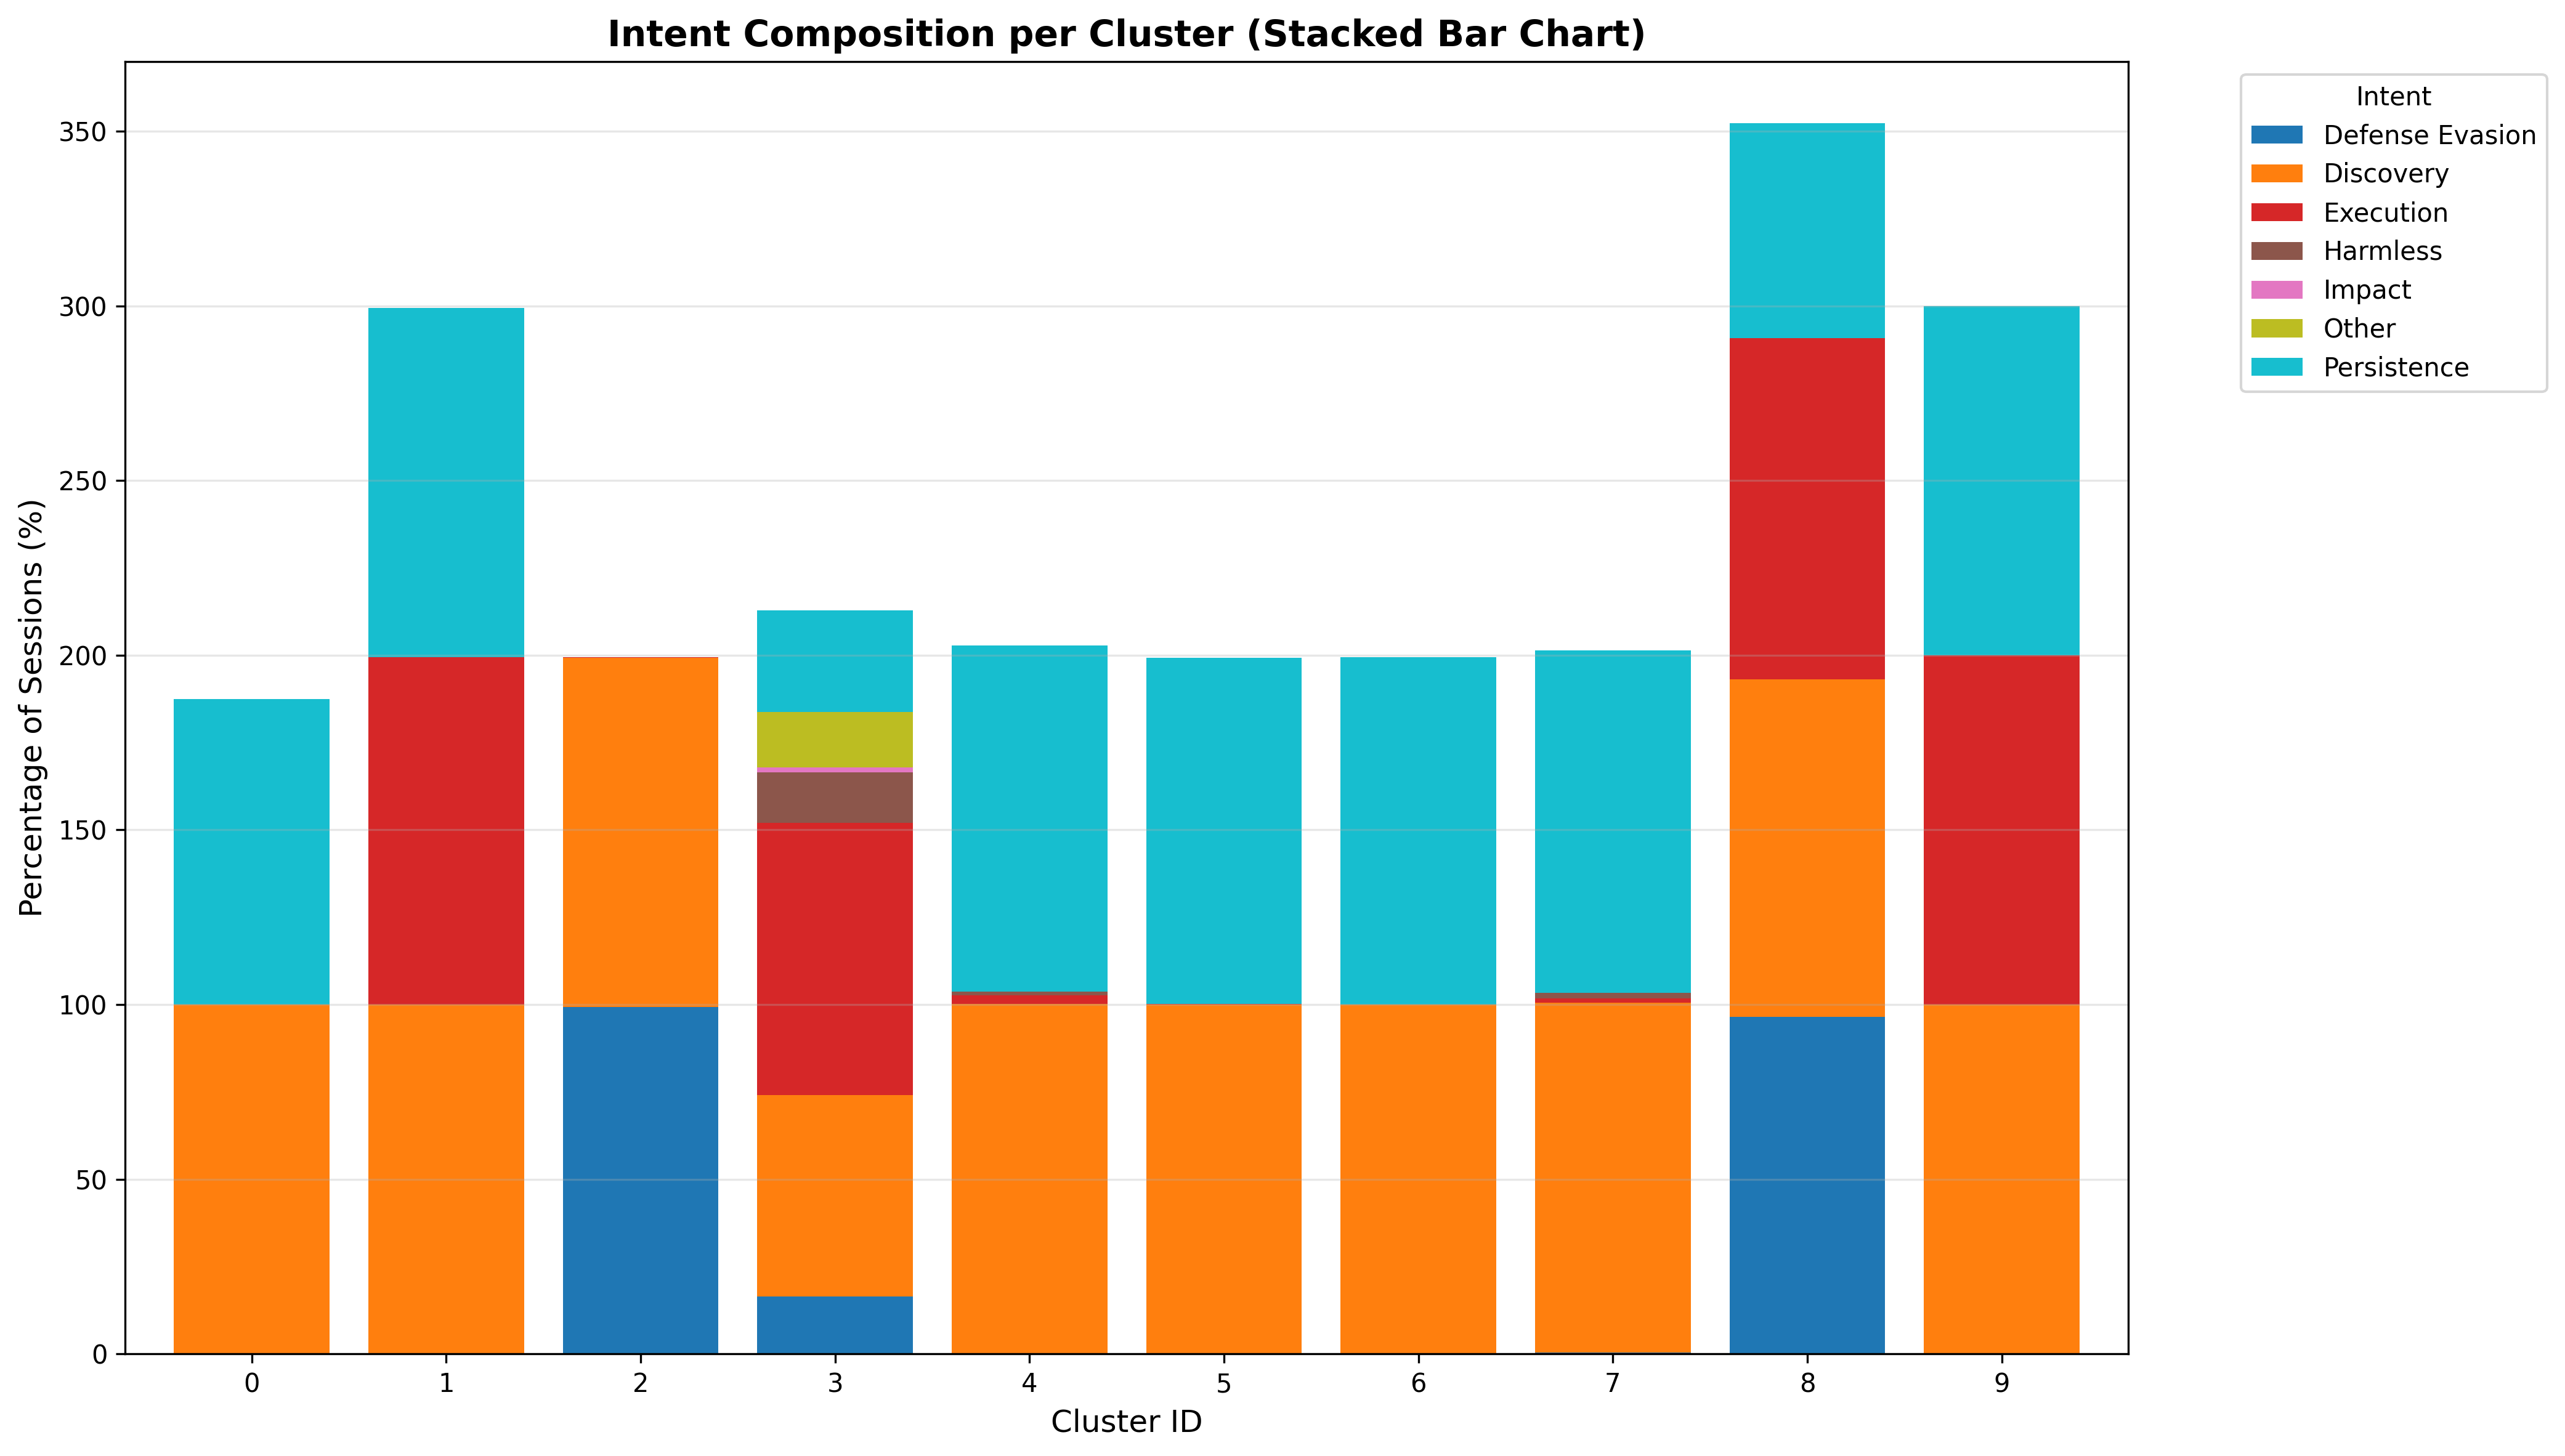
\includegraphics[width=0.85\textwidth]{results/plots/section3/intent_composition_stacked.png}
\caption{Intent composition per cluster showing percentage contribution of each MITRE ATT\&CK intent. Discovery (orange) and Persistence (cyan) dominate most clusters, with Execution (red) and Defense Evasion (blue) appearing in multi-tactic clusters. Stacked percentages exceed 100\% due to multi-label annotation.}
\label{fig:intent_composition_stacked}
\end{figure}

\FloatBarrier
\clearpage
%% ============================================================
%% APPENDIX D: BERT DETAILS
%% ============================================================
\section{Extended BERT Analysis}
\addcontentsline{toc}{section}{Appendix D: Extended BERT Analysis}

This appendix presents the full set of training, evaluation, and test details for the BERT model, offering additional context beyond the main results.

\subsection{Additional Training Visualizations}
\label{appendix:D1}
\addcontentsline{toc}{subsection}{D.1 Additional Training Visualizations}

%DELETED - Useless details
% \begin{figure}[htbp]
%   \centering
%   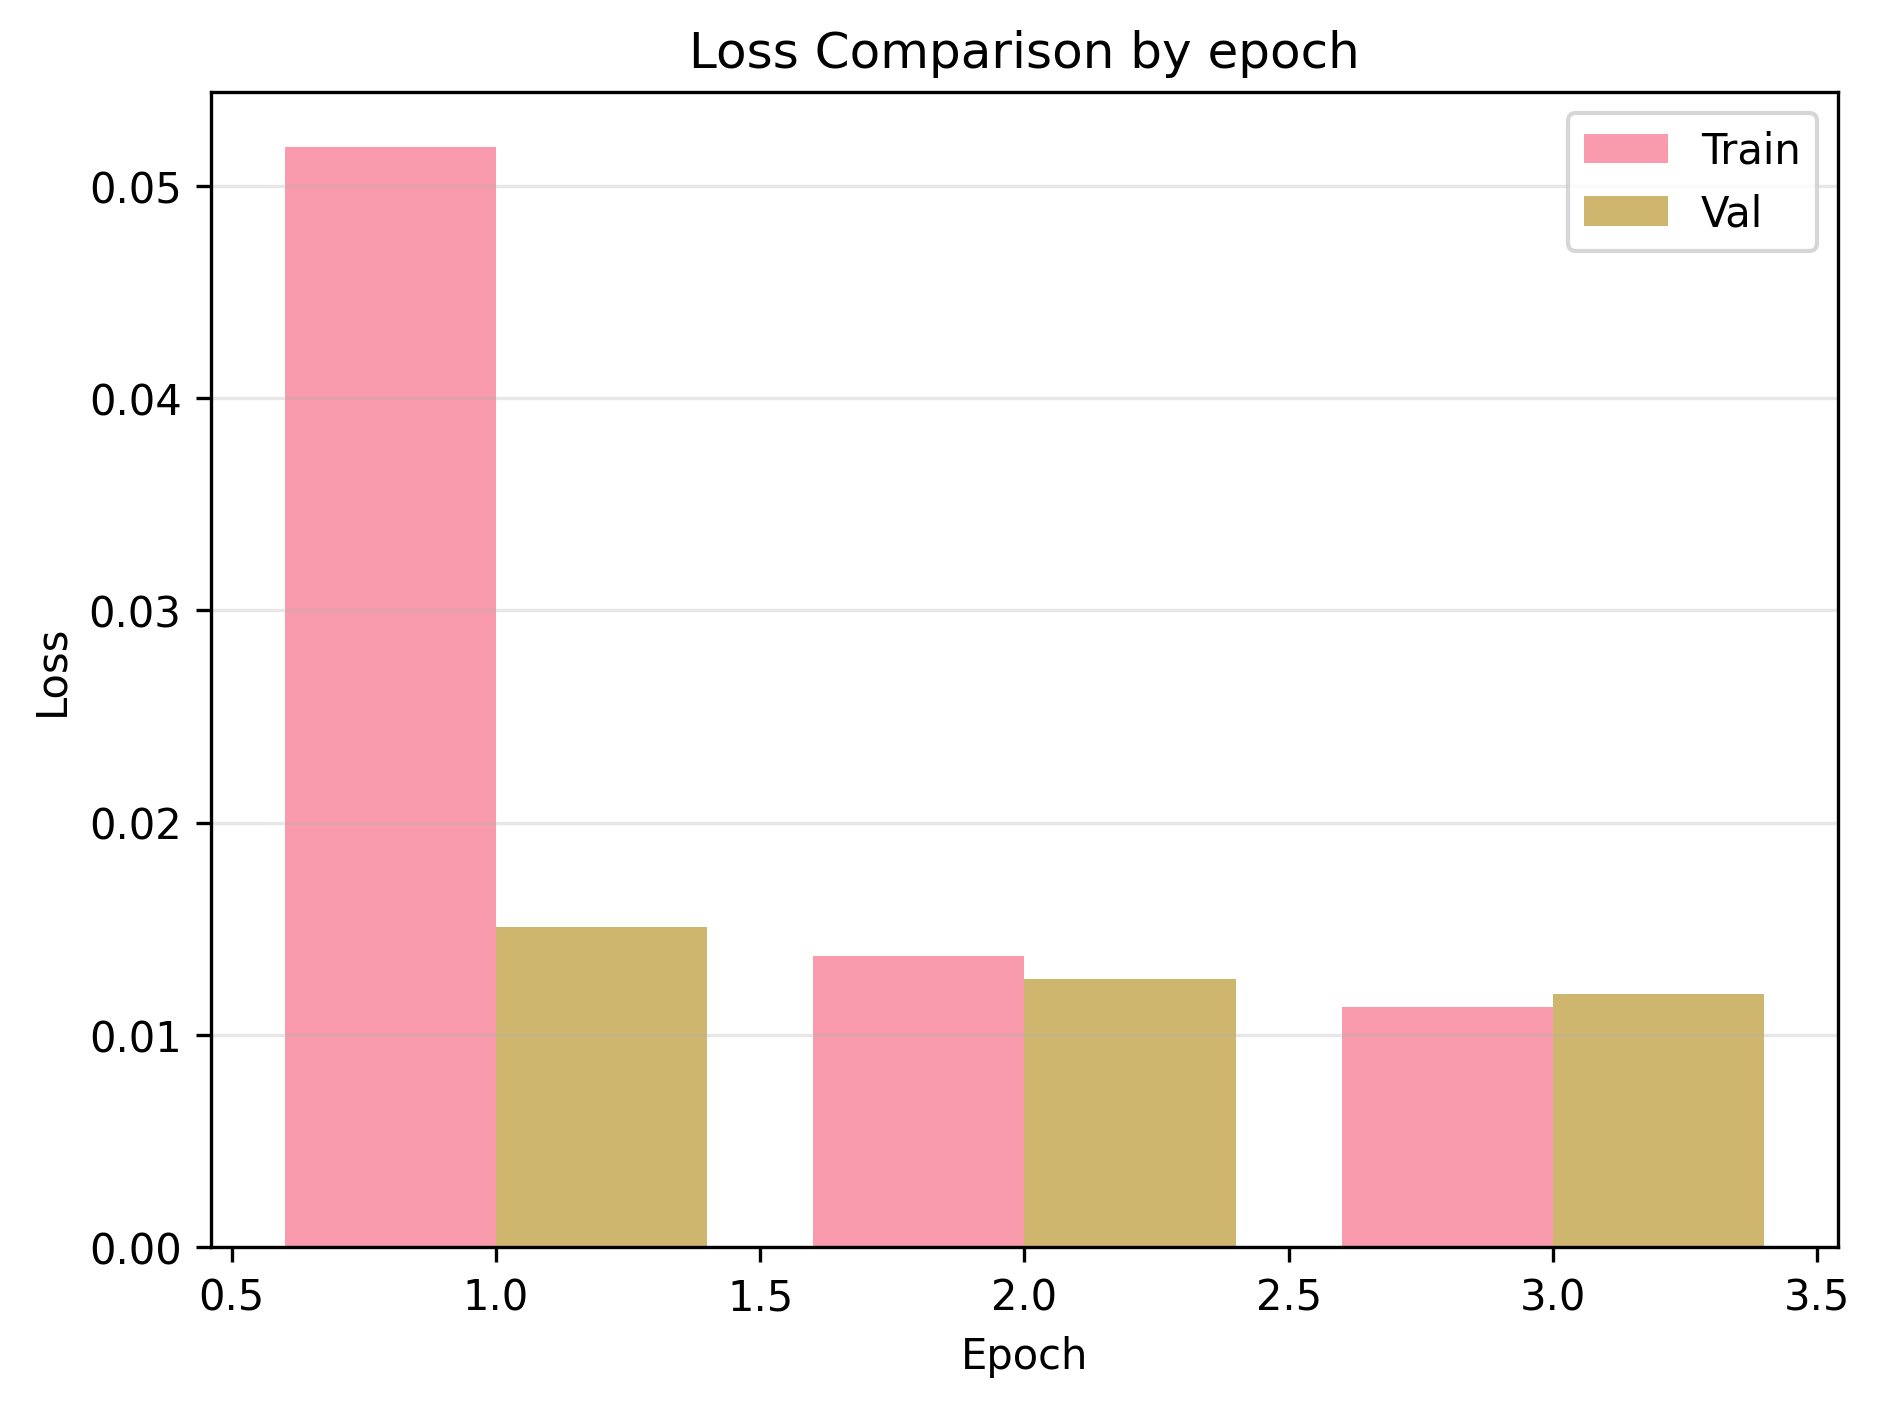
\includegraphics[width=0.7\textwidth]{results/plots/section4/loss_comparison.png}
%   \caption{Comparison of loss functions for multi-label classification.}
%   \label{fig:loss_comp_appendix}
% \end{figure}

\begin{figure}[htbp]
\centering
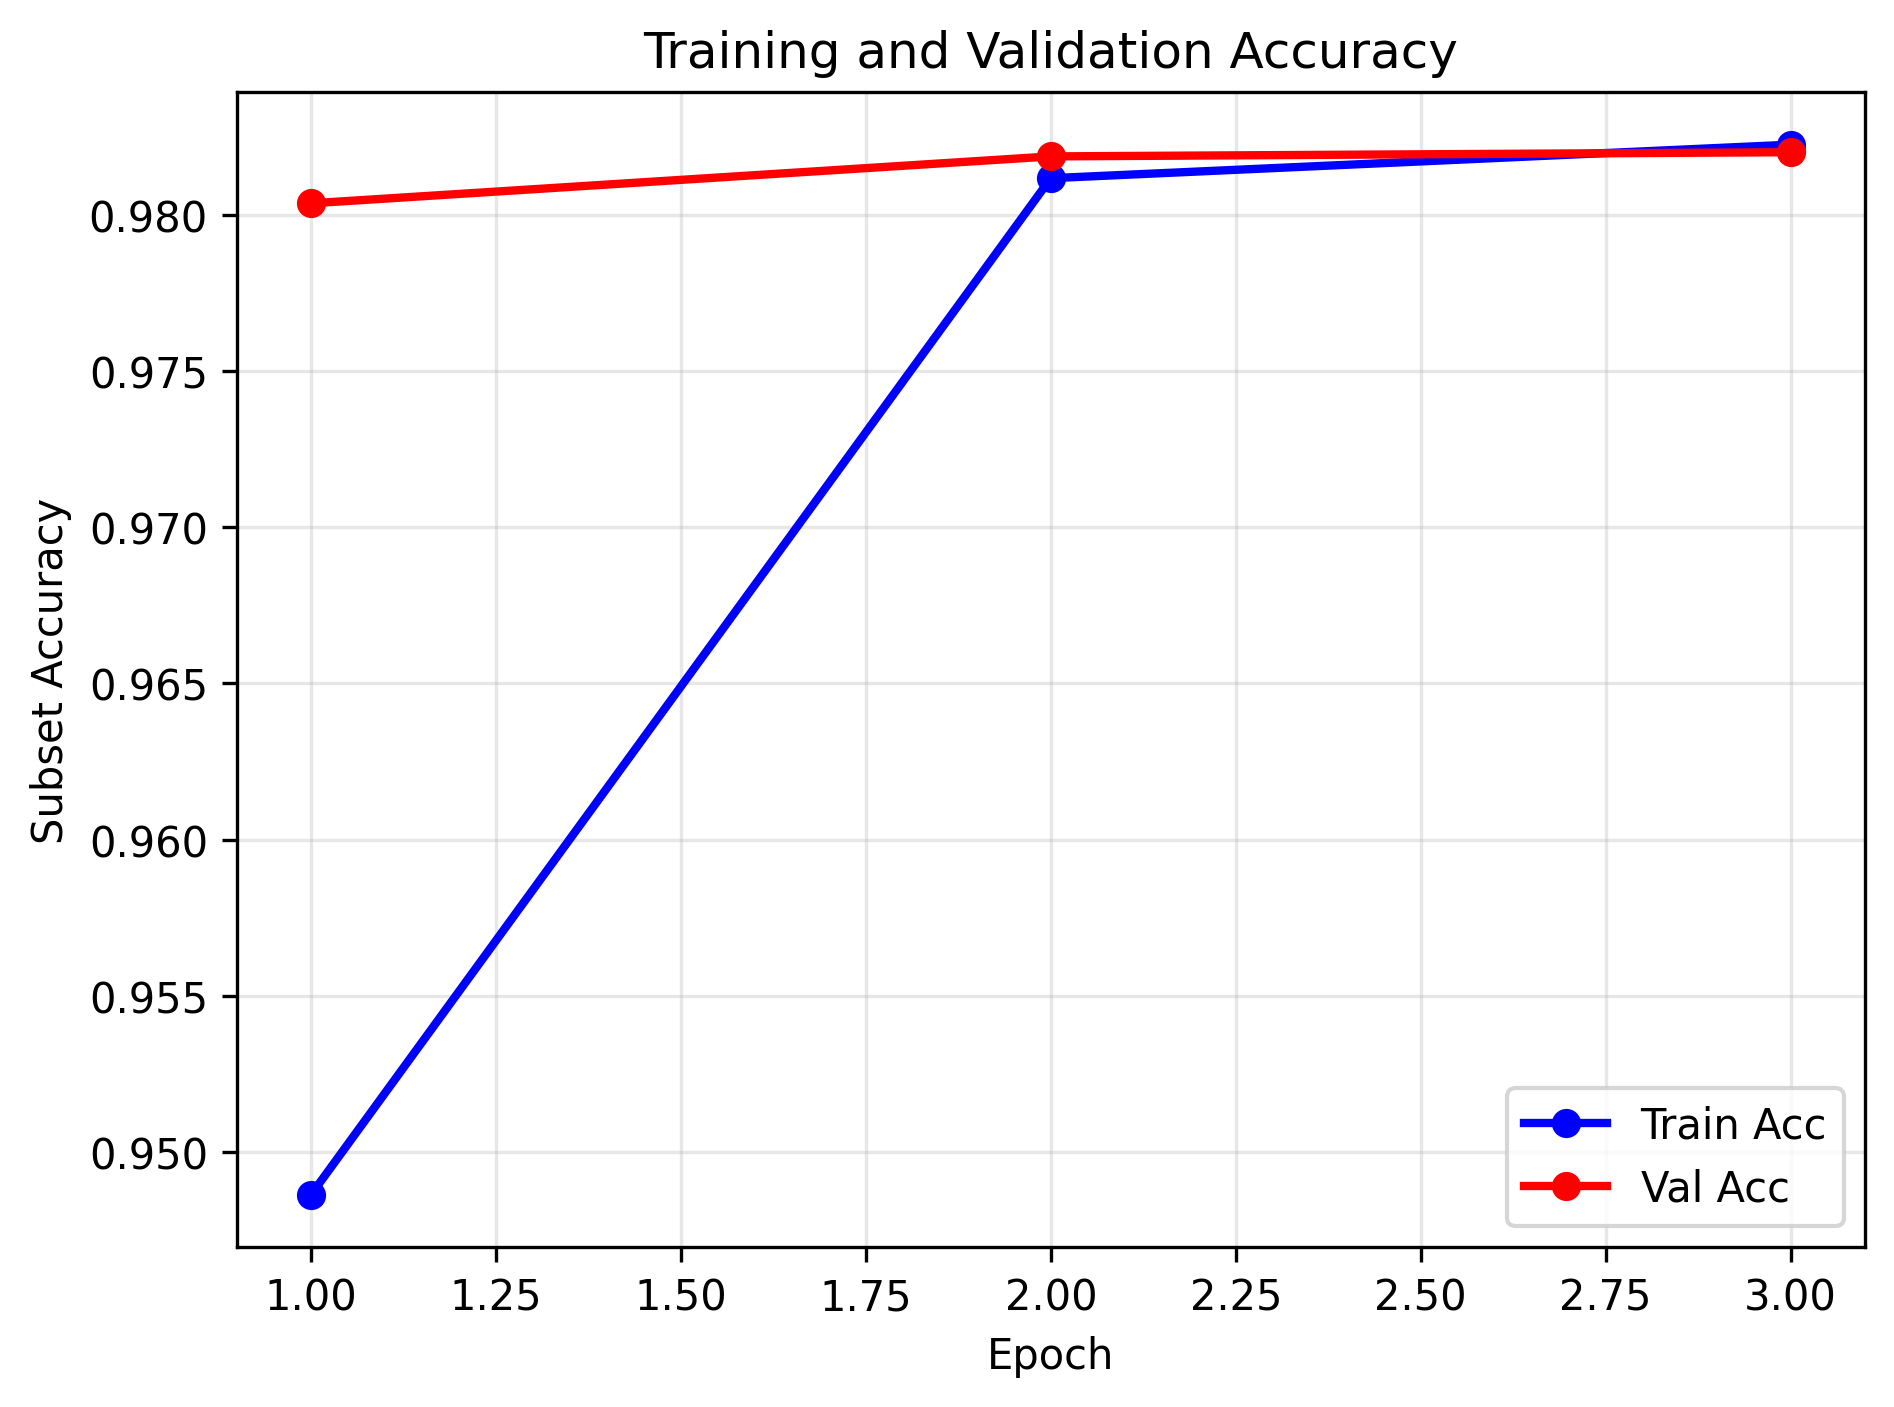
\includegraphics[width=0.55\textwidth]{results/plots/section4/accuracy_curve.png}
\caption{Training and validation accuracy over 3 epochs, showing consistent improvement and early convergence.}
\label{fig:accuracy_curves}
\end{figure}

\begin{figure}[htbp]
\centering
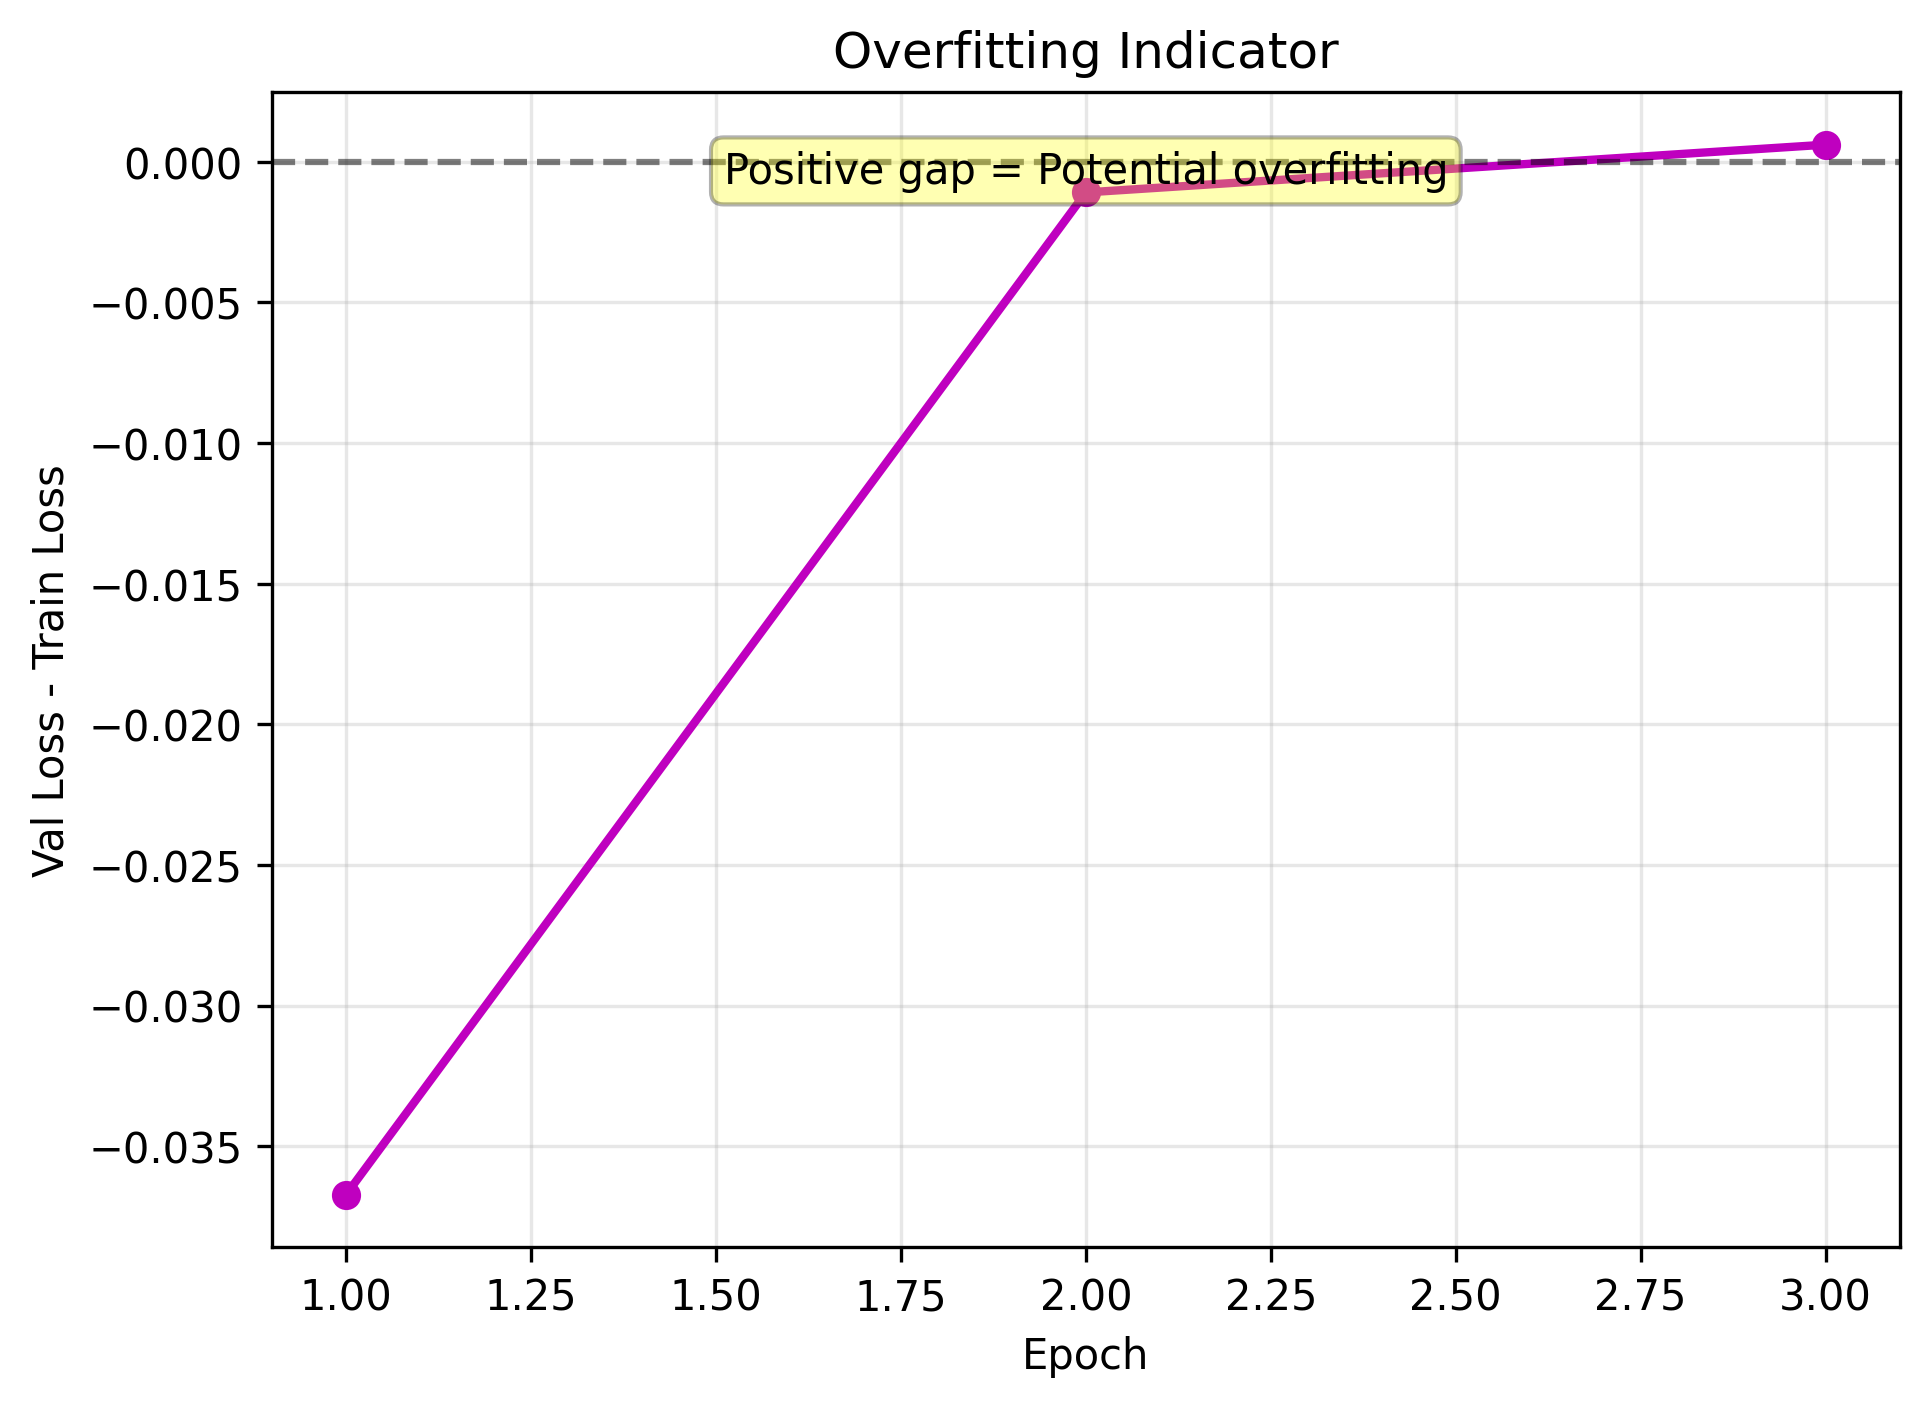
\includegraphics[width=0.6\textwidth]{results/plots/section4/overfitting_indicator.png}
\caption{Overfitting indicator showing the gap between validation and training loss converging to near zero, demonstrating the model's consistent generalization capability}
\label{fig:overfitting}
\end{figure}

\FloatBarrier

\subsection{Detailed Performance Metrics by Intent}
\label{appendix:D2}
\addcontentsline{toc}{subsection}{D.2 Detailed Performance Metrics by Intent}

Table~\ref{tab:detailed_metrics} provides comprehensive per-intent metrics, while Figures~\ref{fig:metrics_comp}, \ref{fig:precision_recall}, and \ref{fig:roc_curve} show detailed visualizations of model performance across all intent categories.

\begin{table}[h]
\centering
\caption{Detailed performance metrics by intent (from test set)}
\label{tab:detailed_metrics}
\begin{tabular}{@{}lrrrrr@{}}
\toprule
\textbf{Intent} & \textbf{Samples} & \textbf{Precision} & \textbf{Recall} & \textbf{F1-Score} & \textbf{\%} \\
\midrule
Persistence   & 42,281 & 0.9994 & 0.9996 & 0.9995 & 90.72\% \\
Discovery     & 46,433 & 1.0000 & 0.9998 & 0.9999 & 99.63\% \\
Defense Evasion & 3,760 & 0.9935 & 0.9737 & 0.9835 & 8.07\% \\
Execution     & 18,512 & 0.9933 & 0.9888 & 0.9909 & 39.72\% \\
Impact        & 2      & 0.0000 & 0.0000 & 0.0000 & 0.004\% \\
Other         & 67     & 1.0000 & 0.9851 & 0.9925 & 0.14\% \\
Harmless      & 458    & 0.6800 & 0.2227 & 0.3355 & 0.98\% \\
\bottomrule
\end{tabular}
\end{table}

\begin{figure}[htbp]
\centering
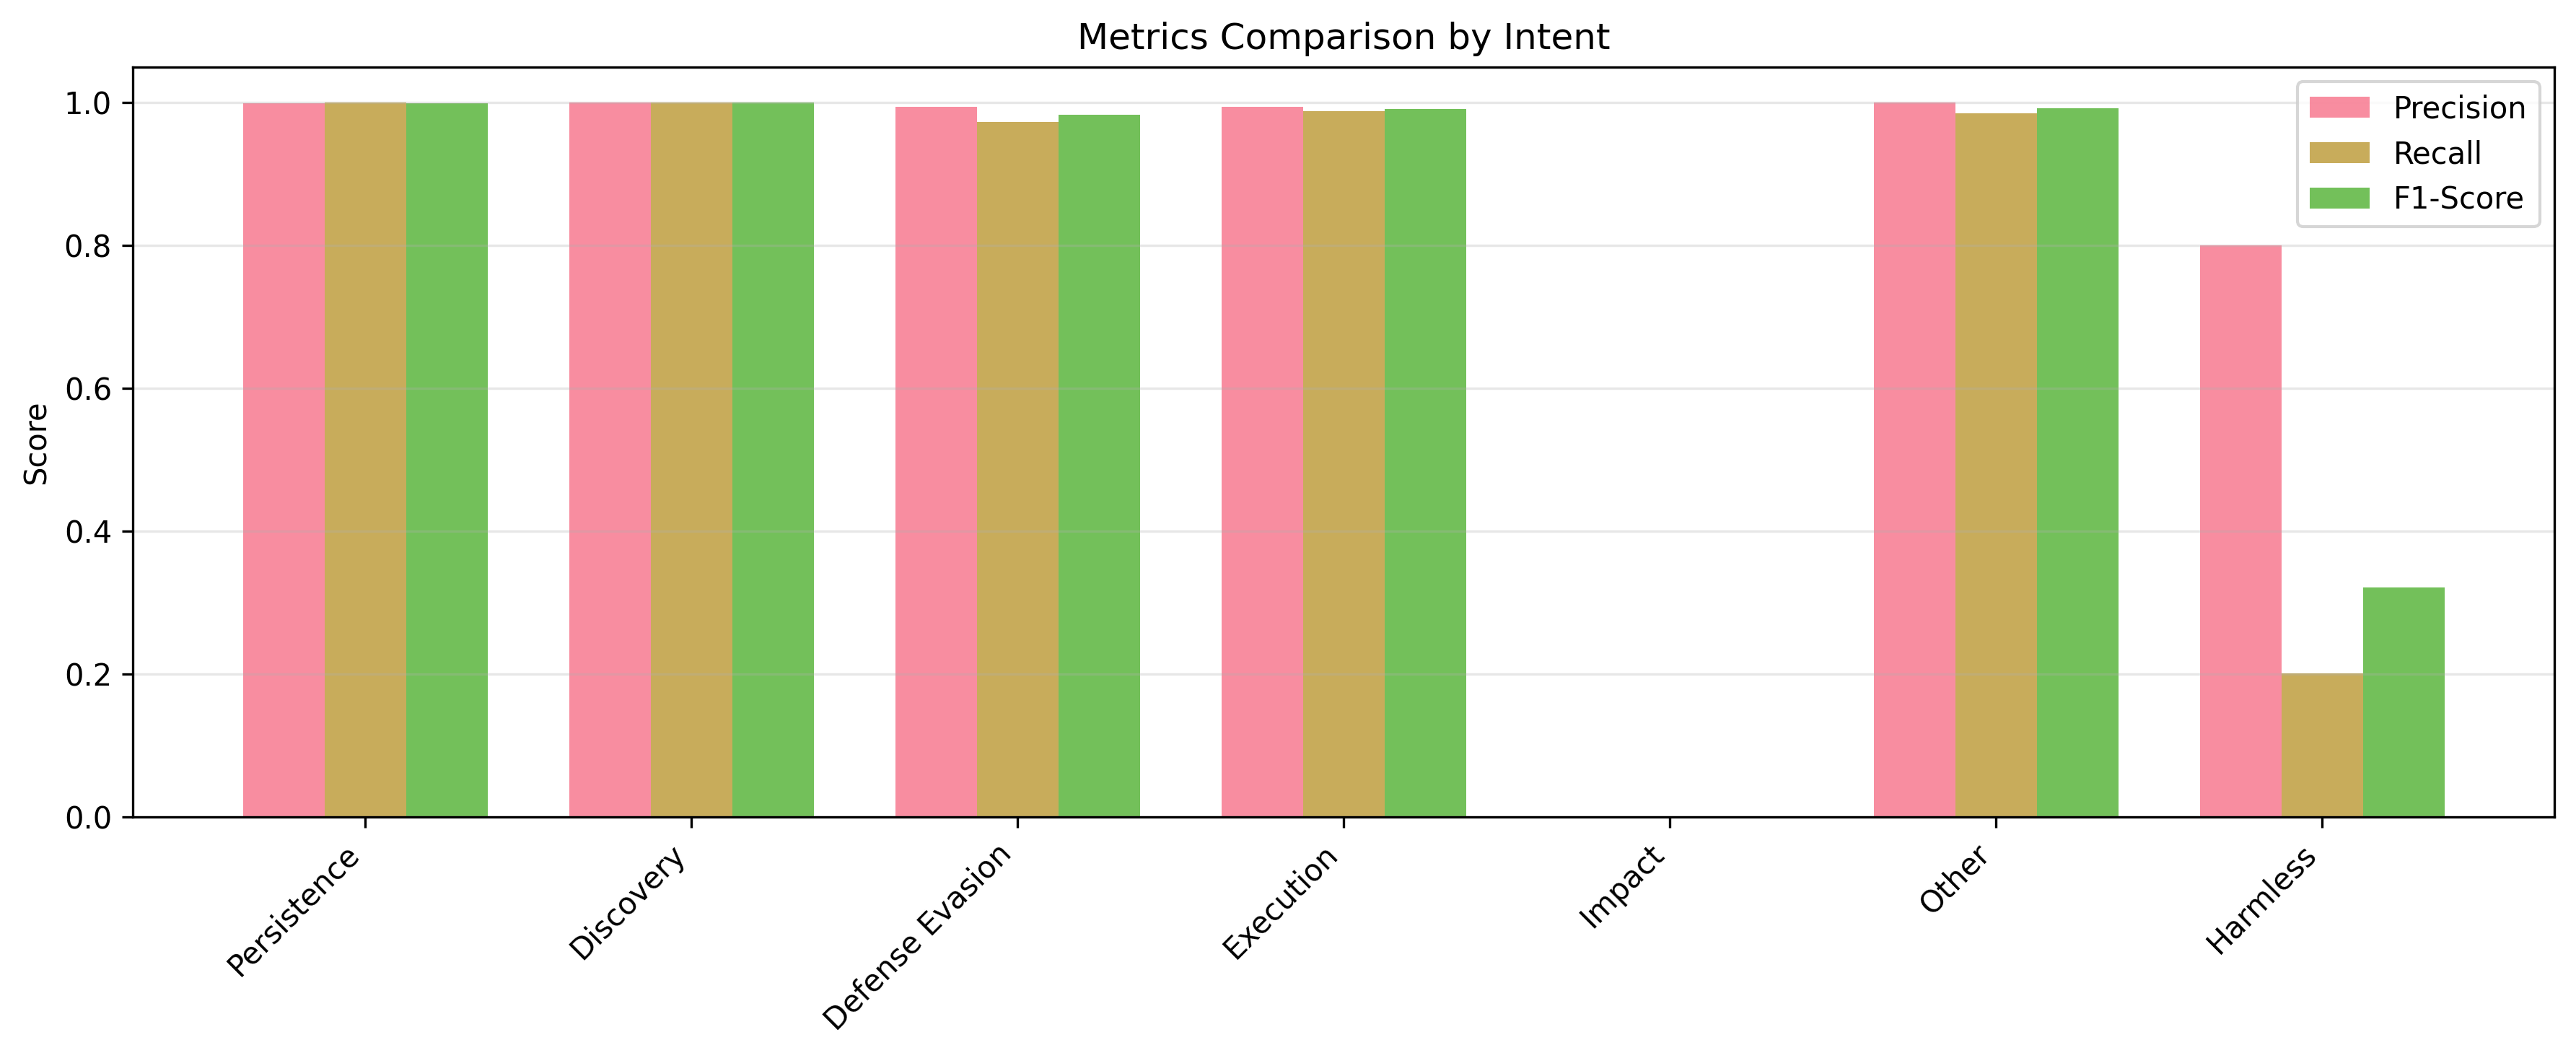
\includegraphics[width=0.8\textwidth]{results/plots/section4/metrics_comparison.png}
\caption{Precision, recall, and F1-score comparison across all intent categories.}
\label{fig:metrics_comp}
\end{figure}

\begin{figure}[htbp]
\centering
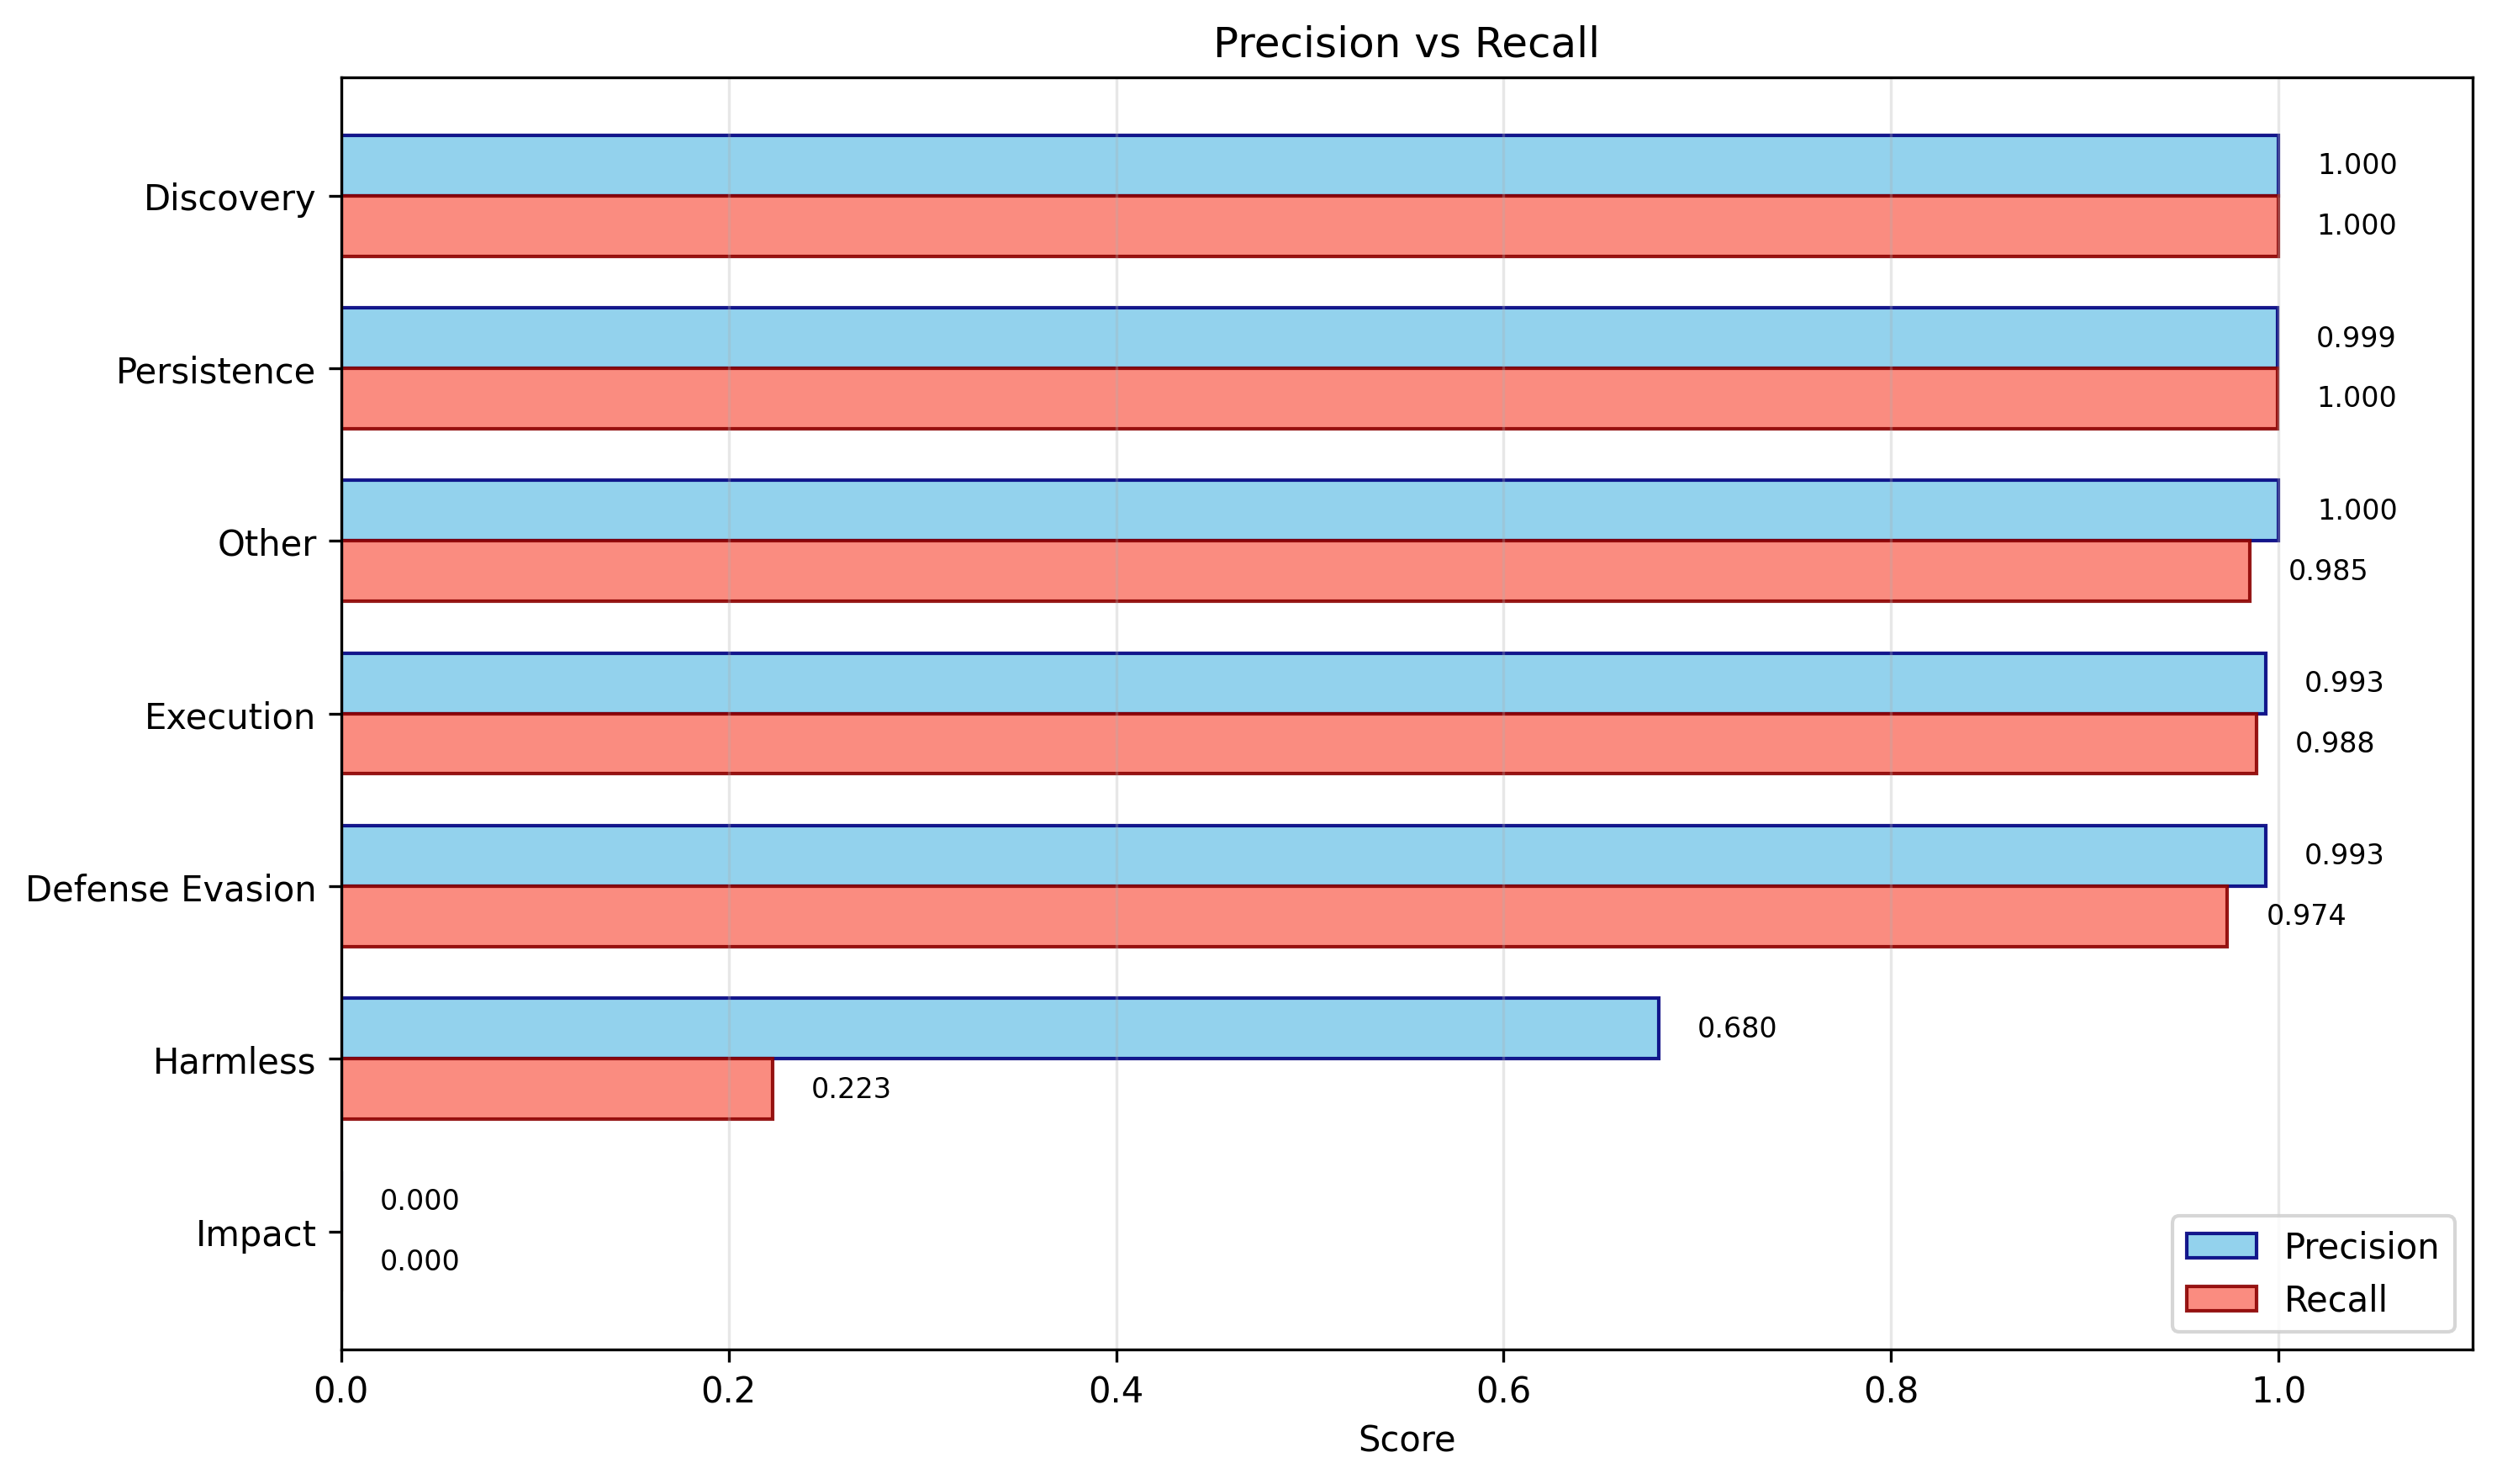
\includegraphics[width=0.75\textwidth]{results/plots/section4/precision_recall_comparison.png}
\caption{Precision vs recall showing trade-offs for each intent. Harmless shows high precision (0.68) but very low recall (0.22), indicating conservative predictions.}
\label{fig:precision_recall}
\end{figure}

\begin{figure}[htbp]
\centering
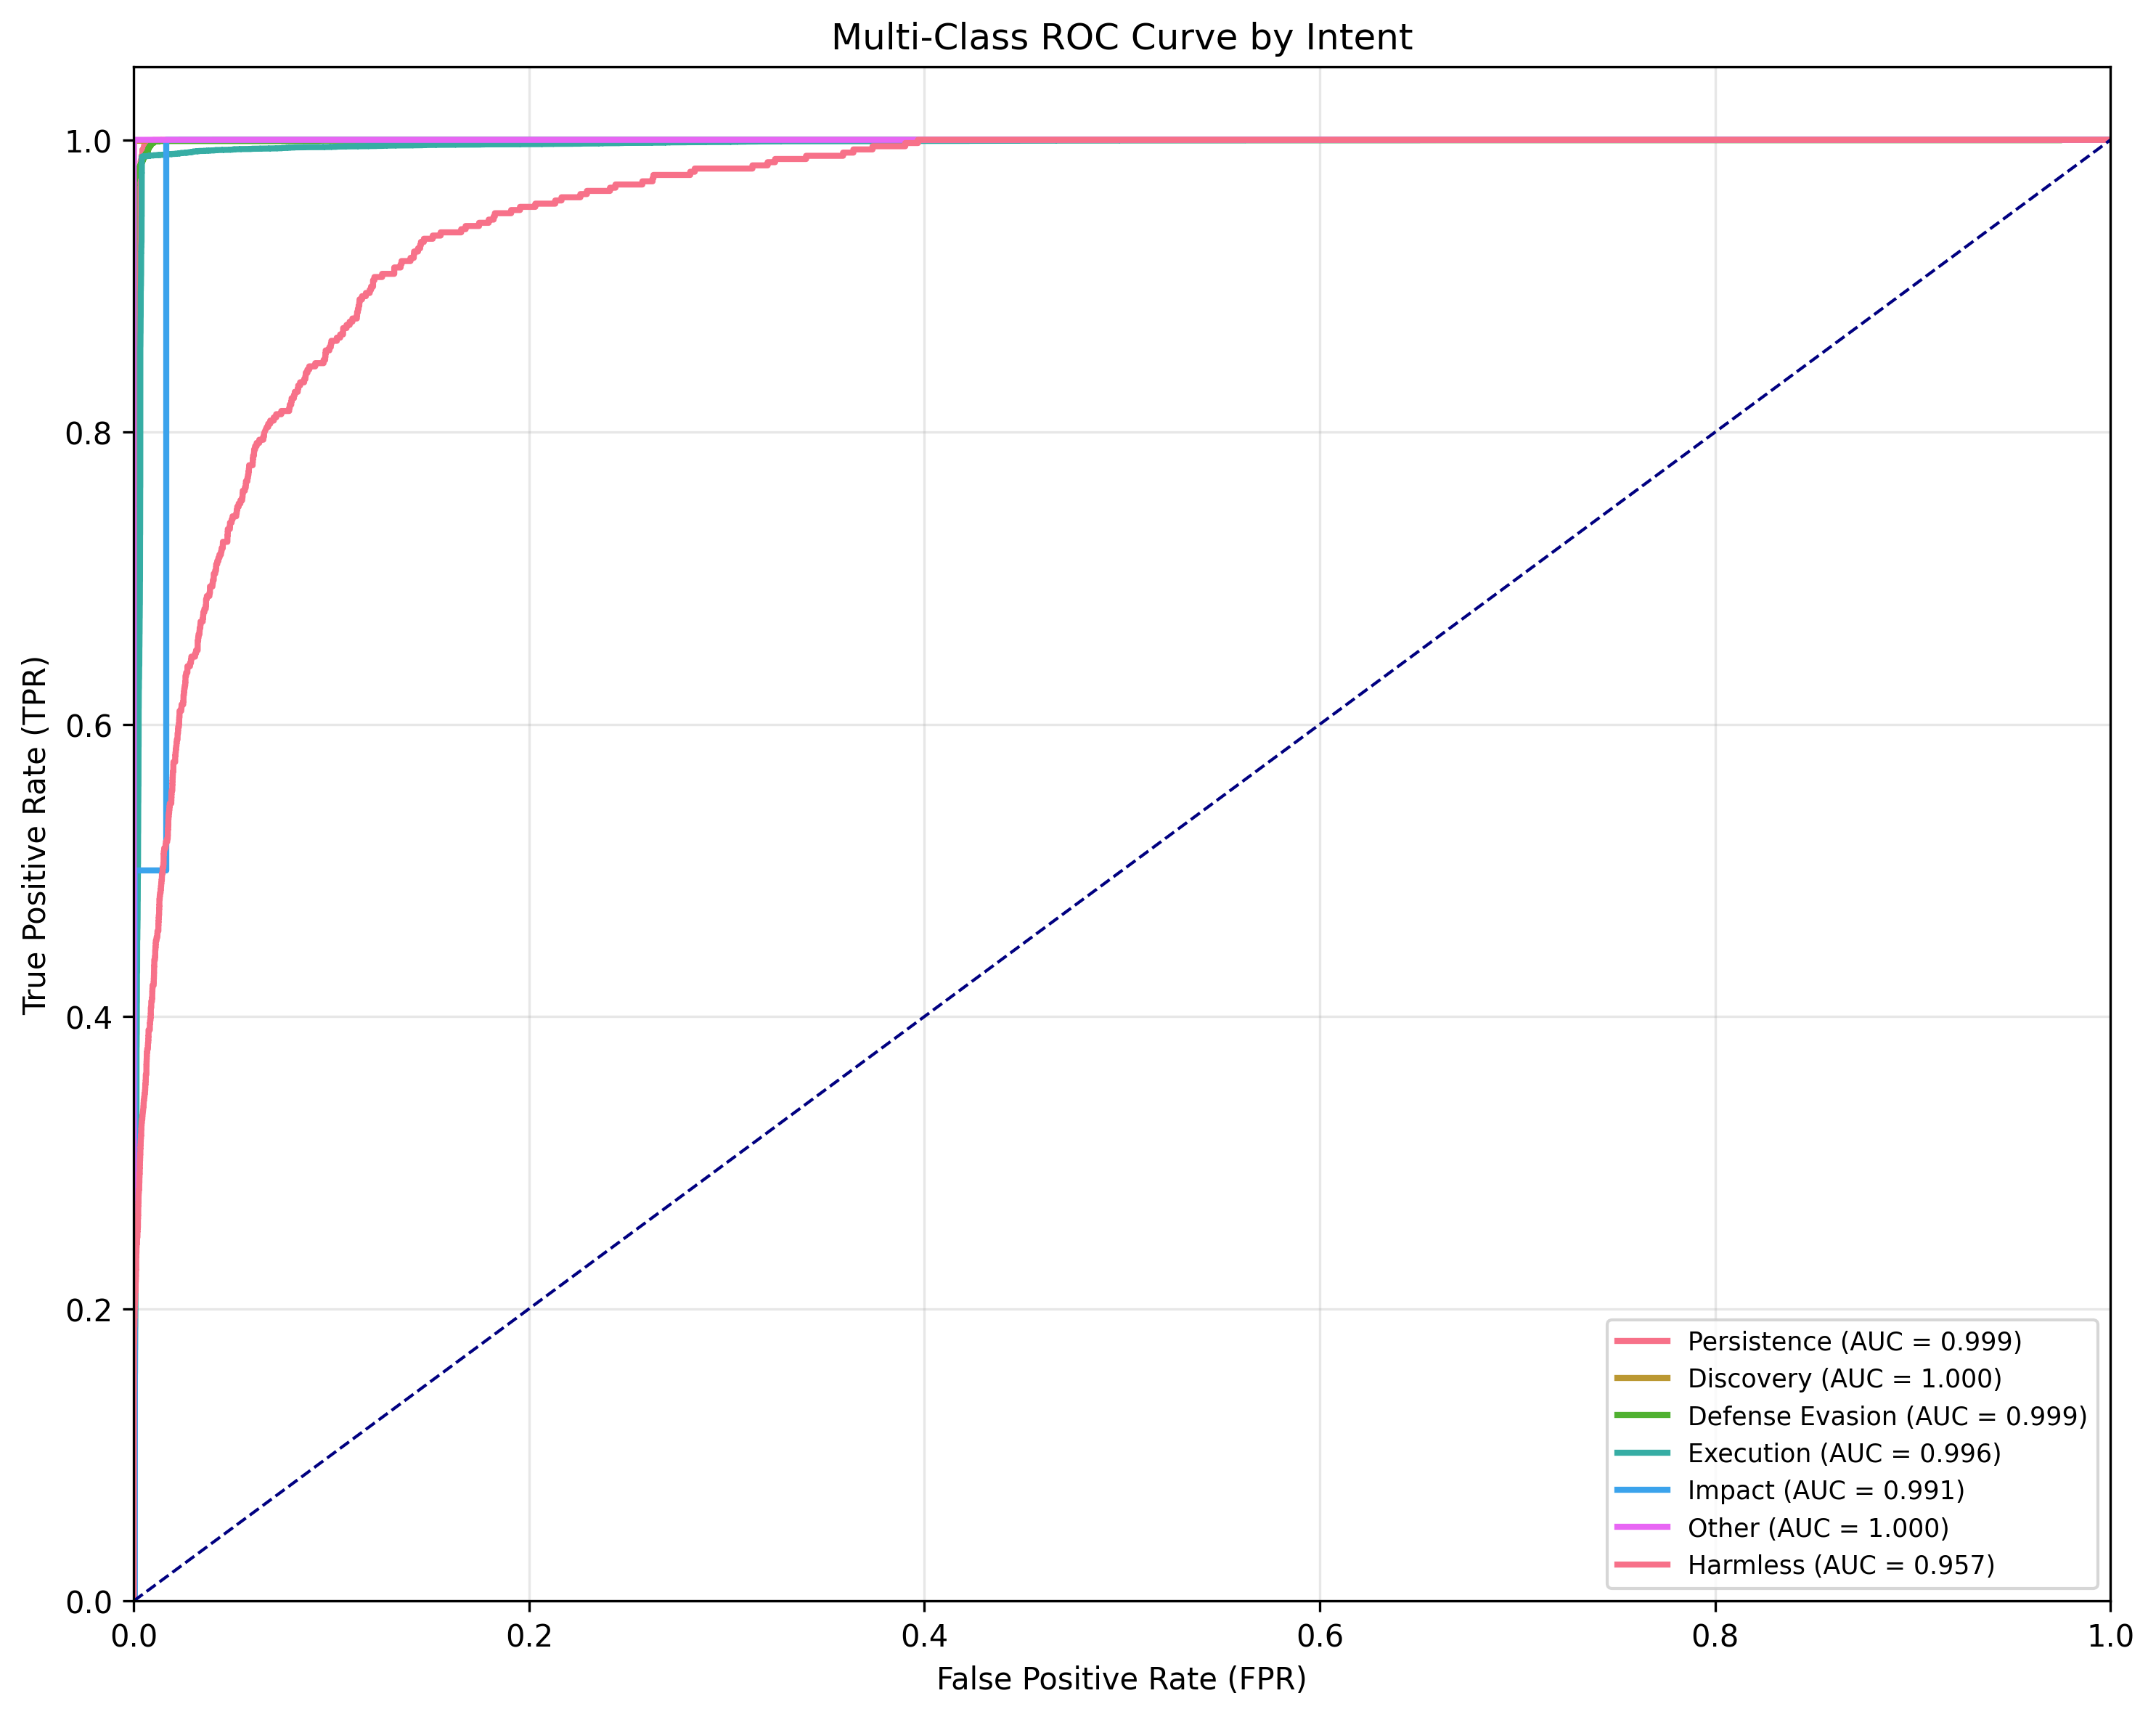
\includegraphics[width=0.75\textwidth]{results/plots/section4/roc_curve_final.png}
\caption{Multi-class ROC curves showing excellent discrimination for all intents including Harmless (AUC: 0.958), demonstrating that the model learns meaningful features even when decision thresholds are suboptimal due to extreme imbalance.}
\label{fig:roc_curve}
\end{figure}


%% ============================================================
%% APPENDIX E: IMPLEMENTATION AND REPRODUCIBILITY
%% ============================================================
\FloatBarrier
\section{Implementation and Reproducibility Notes}
\addcontentsline{toc}{section}{Appendix E: Implementation and Reproducibility Notes}

This appendix summarizes implementation details to support reproducibility of all
experiments reported in the main document.

\subsection{Software Environment}
\begin{itemize}
  \item \textbf{Programming Language}: Python 3.8+
  \item \textbf{Machine Learning}: scikit-learn 1.0+, NumPy 1.21+, Pandas 1.3+
  \item \textbf{Deep Learning}: PyTorch 1.10+, HuggingFace Transformers 4.18+
  \item \textbf{Visualization}: Matplotlib 3.4+, Seaborn 0.11+, WordCloud 1.8+
  \item \textbf{Hardware}: CPU (traditional ML), NVIDIA GPU with CUDA 11.3+ (BERT)
\end{itemize}

\subsection{Data Processing}
\begin{itemize}
  \item \textbf{Text Representation}: TF-IDF with min\_df=5, max\_features=5000
  \item \textbf{Train-Test Split}: 80\% training / 20\% testing, stratified by intent
  \item \textbf{Random Seed}: 42 (consistent across all experiments)
  \item \textbf{Multi-label Encoding}: Binary relevance (one binary classifier per intent)
\end{itemize}

\subsection{Model Hyperparameters}
\begin{itemize}
  \item \textbf{Logistic Regression}: C=1.0, penalty='l2', solver='lbfgs', class\_weight='balanced'
  \item \textbf{SVM}: C=1.0, kernel='linear', class\_weight='balanced'
  \item \textbf{K-Means}: k=10, init='k-means++', n\_init=10, random\_state=42
  \item \textbf{Hierarchical}: n\_clusters=10, linkage='ward', affinity='euclidean'
  \item \textbf{BERT}: bert-base-uncased, lr=2e-5, batch\_size=32, epochs=3, max\_length=256
\end{itemize}

\end{document}
